%%%%%%%%%%%%%%%%%%%% book.tex %%%%%%%%%%%%%%%%%%%%%%%%%%%%%
%
% sample root file for the chapters of your "monograph"
%
% Use this file as a template for your own input.
%
%%%%%%%%%%%%%%%% Springer-Verlag %%%%%%%%%%%%%%%%%%%%%%%%%%


% RECOMMENDED %%%%%%%%%%%%%%%%%%%%%%%%%%%%%%%%%%%%%%%%%%%%%%%%%%%
\documentclass[graybox,envcountchap,sectrefs]{svmono}


\usepackage{mathptmx}
 

\usepackage{makeidx}         % allows index generation

\usepackage{graphicx,epstopdf}        % standard LaTeX graphics tool

\usepackage{epstopdf}
\epstopdfsetup{update} % only regenerate pdf files when eps file is newer
                             % when including figure files
\usepackage{multicol}        % used for the two-column index
\usepackage[bottom]{footmisc}% places footnotes at page bottom

\usepackage{newtxtext}       % 
\usepackage[varvw]{newtxmath}       % selects Times Roman as basic font

\usepackage{soul}               % strike-through

\usepackage{hyperref}        % Springer recommendation - remocve when showidx active

\newcommand{\lingform}[1]{\textit{\texttt{#1}}}
\newcommand{\lingformquote}[1]{\texttt{#1}}
\newcommand{\code}[1]{\texttt{#1}}
\newcommand{\semantic}[1]{\texttt{#1}}
\newcommand{\scare}[1]{`#1'}
\newcommand{\blankline}{\vspace{\baselineskip}}
\newcommand{\lineacross}{\rule{\linewidth}{1pt}}

\newcommand{\personal}[1]{\medskip\noindent\fbox{\begin{minipage}{\textwidth}\textbf{Personal Note:} #1\end{minipage}}\medskip}



\makeindex             % used for the subject index


%%%%%%%%%%%%%%%%%%%%%%%%%%%%%%%%%%%%%%%%%%%%%%%%%%%%%%%%%%%%%%%%%%%%%

\begin{document}

\author{Ehud Reiter}
\title{Natural Language Generation}
%\subtitle{-- Monograph --}
\maketitle

\frontmatter%%%%%%%%%%%%%%%%%%%%%%%%%%%%%%%%%%%%%%%%%%%%%%%%%%%%%%

%\newpage
\section*{Dedication}
\label{sec:dedication}

This thesis is dedicated to:

\begin{itemize}
    \item Anna M., I am profoundly grateful for her endless patience, support, and belief in me;
    \item my family, whose unwavering encouragement has always been unconditional;
    \item friends and colleagues, being part of a group of wonderful people has given me extra motivation and lots of smiles. To future PhD students, try to exchange and share ideas, do not isolate yourself.
\end{itemize}

\section*{Acknowledgment}
This work was supported by the National Natural Science Foundation of China (62441239,~U23A20319,~62172056,~62472394,~62192784, \\ U22B2038) as well as the 8th Young Elite Scientists Sponsorship Program by CAST (2022QNRC001).

%\include{foreword}
\chapter*{Preface}

Artificial intelligence commonly refers to the science and engineering of artificial systems that can carry out tasks generally associated with requiring aspects of human intelligence, such as playing games, translating languages, and driving cars.
In recent years, there have been exciting advances in learning-based, data-driven approaches towards AI, and machine learning and deep learning have enabled computer systems to perceive the world in unprecedented ways.
Reinforcement learning has enabled breakthroughs in complex games such as Go and challenging robotics tasks such as quadrupedal locomotion.

A key aspect of intelligence is to not only make predictions, but reason about the {\em uncertainty} in these predictions, and to consider this uncertainty when making decisions.
This is what ``Probabilistic Artificial Intelligence'' is about.
The first part covers probabilistic approaches to machine learning.
We discuss the differentiation between ``epistemic'' uncertainty due to lack of data and ``aleatoric'' uncertainty, which is irreducible and stems, e.g., from noisy observations and outcomes.
We discuss concrete approaches towards probabilistic inference, such as Bayesian linear regression, Gaussian process models and Bayesian neural networks.
Often, inference and making predictions with such models is intractable, and we discuss modern approaches to efficient approximate inference.

The second part of the \course is about taking uncertainty into account in sequential decision tasks.
We consider active learning and Bayesian optimization --- approaches that collect data by proposing experiments that are informative for reducing the epistemic uncertainty.
We then consider reinforcement learning, a rich formalism for modeling agents that learn to act in uncertain environments.
After covering the basic formalism of Markov Decision Processes, we consider modern deep RL approaches that use neural network function approximation.
We close by discussing modern approaches in model-based RL, which harness epistemic and aleatoric uncertainty to guide exploration, while also reasoning about safety.

\section*{Guide to the Reader}

The material covered in this manuscript may support a one semester graduate introduction to probabilistic machine learning and sequential decision-making.
We welcome readers from all backgrounds.
However, we assume familiarity with basic concepts in probability, calculus, linear algebra, and machine learning (e.g., neural networks) as covered in a typical introductory course to machine learning.
In \cref{sec:fundamentals}, we give a gentle introduction to probabilistic inference, which serves as the foundation for the rest of the manuscript.
As part of this first chapter, we also review key concepts from probability theory.
We provide a chapter reviewing key concepts of further mathematical background in the back of the manuscript.

Throughout the manuscript, we focus on key concepts and ideas rather than their historical development.
We encourage you to consult the provided references for further reading and historical context to delve deeper into the covered topics.

\ifthenelse{\boolean{manuscript}}{}{
  Accompanying this manuscript, we provide an extensive set of curated examples as Jupyter notebooks which you can run and play with.
  You can find them at: \\
  \url{https://gitlab.inf.ethz.ch/OU-KRAUSE/pai-demos}.
}

Finally, we have included a set of exercises at the end of each chapter.
When we highlight an exercise throughout the text, we use this question mark: \exerciserefmark{properties_of_probability} --- so don't be surprised when you stumble upon it.
You will find solutions to all exercises in the back of the manuscript.

We hope you will find this resource useful.

\section*{Contributing}

We encourage you to raise issues and suggest fixes for anything you think can be improved.
We are thankful for any such feedback! \\
\textsc{Contact:} \href{mailto:pai-script@lists.inf.ethz.ch}{pai-script@lists.inf.ethz.ch}
\ifthenelse{\boolean{manuscript}}{}{\\ \textsc{Repository:} \url{https://gitlab.inf.ethz.ch/OU-KRAUSE/pai-script}}


\section*{Acknowledgements}

We are grateful to Sebastian Curi for creating the original Jupyter notebooks that accompany the course at ETH Zürich and which were instrumental in the creation of many figures.
We thank Hado van Hasselt for kindly contributing \cref{fig:maximization_bias}, and thank Tuomas Haarnoja~\citep{haarnoja2018soft} and Roberto Calandra~\citep{chua2018deep} for kindly agreeing to have their figures included in this manuscript.
Furthermore, many of the exercises in these notes are adapted from iterations of the course at ETH Zürich.
Special thanks to all instructors that contributed to the course material over the years.
We also thank all students of the course in the Fall of 2022, 2023, and 2024 who provided valuable feedback on various iterations of this manuscript and corrected many mistakes.
Finally, we thank Zhiyuan Hu, Shyam Sundhar Ramesh, Leander Diaz-Bone, Nicolas Menet, and Ido Hakimi for proofreading parts of various drafts of this text.



\tableofcontents



\mainmatter%%%%%%%%%%%%%%%%%%%%%%%%%%%%%%%%%%%%%%%%%%%%%%%%%%%%%%%

\section{Introduction}
\label{sec:introduction}
The business processes of organizations are experiencing ever-increasing complexity due to the large amount of data, high number of users, and high-tech devices involved \cite{martin2021pmopportunitieschallenges, beerepoot2023biggestbpmproblems}. This complexity may cause business processes to deviate from normal control flow due to unforeseen and disruptive anomalies \cite{adams2023proceddsriftdetection}. These control-flow anomalies manifest as unknown, skipped, and wrongly-ordered activities in the traces of event logs monitored from the execution of business processes \cite{ko2023adsystematicreview}. For the sake of clarity, let us consider an illustrative example of such anomalies. Figure \ref{FP_ANOMALIES} shows a so-called event log footprint, which captures the control flow relations of four activities of a hypothetical event log. In particular, this footprint captures the control-flow relations between activities \texttt{a}, \texttt{b}, \texttt{c} and \texttt{d}. These are the causal ($\rightarrow$) relation, concurrent ($\parallel$) relation, and other ($\#$) relations such as exclusivity or non-local dependency \cite{aalst2022pmhandbook}. In addition, on the right are six traces, of which five exhibit skipped, wrongly-ordered and unknown control-flow anomalies. For example, $\langle$\texttt{a b d}$\rangle$ has a skipped activity, which is \texttt{c}. Because of this skipped activity, the control-flow relation \texttt{b}$\,\#\,$\texttt{d} is violated, since \texttt{d} directly follows \texttt{b} in the anomalous trace.
\begin{figure}[!t]
\centering
\includegraphics[width=0.9\columnwidth]{images/FP_ANOMALIES.png}
\caption{An example event log footprint with six traces, of which five exhibit control-flow anomalies.}
\label{FP_ANOMALIES}
\end{figure}

\subsection{Control-flow anomaly detection}
Control-flow anomaly detection techniques aim to characterize the normal control flow from event logs and verify whether these deviations occur in new event logs \cite{ko2023adsystematicreview}. To develop control-flow anomaly detection techniques, \revision{process mining} has seen widespread adoption owing to process discovery and \revision{conformance checking}. On the one hand, process discovery is a set of algorithms that encode control-flow relations as a set of model elements and constraints according to a given modeling formalism \cite{aalst2022pmhandbook}; hereafter, we refer to the Petri net, a widespread modeling formalism. On the other hand, \revision{conformance checking} is an explainable set of algorithms that allows linking any deviations with the reference Petri net and providing the fitness measure, namely a measure of how much the Petri net fits the new event log \cite{aalst2022pmhandbook}. Many control-flow anomaly detection techniques based on \revision{conformance checking} (hereafter, \revision{conformance checking}-based techniques) use the fitness measure to determine whether an event log is anomalous \cite{bezerra2009pmad, bezerra2013adlogspais, myers2018icsadpm, pecchia2020applicationfailuresanalysispm}. 

The scientific literature also includes many \revision{conformance checking}-independent techniques for control-flow anomaly detection that combine specific types of trace encodings with machine/deep learning \cite{ko2023adsystematicreview, tavares2023pmtraceencoding}. Whereas these techniques are very effective, their explainability is challenging due to both the type of trace encoding employed and the machine/deep learning model used \cite{rawal2022trustworthyaiadvances,li2023explainablead}. Hence, in the following, we focus on the shortcomings of \revision{conformance checking}-based techniques to investigate whether it is possible to support the development of competitive control-flow anomaly detection techniques while maintaining the explainable nature of \revision{conformance checking}.
\begin{figure}[!t]
\centering
\includegraphics[width=\columnwidth]{images/HIGH_LEVEL_VIEW.png}
\caption{A high-level view of the proposed framework for combining \revision{process mining}-based feature extraction with dimensionality reduction for control-flow anomaly detection.}
\label{HIGH_LEVEL_VIEW}
\end{figure}

\subsection{Shortcomings of \revision{conformance checking}-based techniques}
Unfortunately, the detection effectiveness of \revision{conformance checking}-based techniques is affected by noisy data and low-quality Petri nets, which may be due to human errors in the modeling process or representational bias of process discovery algorithms \cite{bezerra2013adlogspais, pecchia2020applicationfailuresanalysispm, aalst2016pm}. Specifically, on the one hand, noisy data may introduce infrequent and deceptive control-flow relations that may result in inconsistent fitness measures, whereas, on the other hand, checking event logs against a low-quality Petri net could lead to an unreliable distribution of fitness measures. Nonetheless, such Petri nets can still be used as references to obtain insightful information for \revision{process mining}-based feature extraction, supporting the development of competitive and explainable \revision{conformance checking}-based techniques for control-flow anomaly detection despite the problems above. For example, a few works outline that token-based \revision{conformance checking} can be used for \revision{process mining}-based feature extraction to build tabular data and develop effective \revision{conformance checking}-based techniques for control-flow anomaly detection \cite{singh2022lapmsh, debenedictis2023dtadiiot}. However, to the best of our knowledge, the scientific literature lacks a structured proposal for \revision{process mining}-based feature extraction using the state-of-the-art \revision{conformance checking} variant, namely alignment-based \revision{conformance checking}.

\subsection{Contributions}
We propose a novel \revision{process mining}-based feature extraction approach with alignment-based \revision{conformance checking}. This variant aligns the deviating control flow with a reference Petri net; the resulting alignment can be inspected to extract additional statistics such as the number of times a given activity caused mismatches \cite{aalst2022pmhandbook}. We integrate this approach into a flexible and explainable framework for developing techniques for control-flow anomaly detection. The framework combines \revision{process mining}-based feature extraction and dimensionality reduction to handle high-dimensional feature sets, achieve detection effectiveness, and support explainability. Notably, in addition to our proposed \revision{process mining}-based feature extraction approach, the framework allows employing other approaches, enabling a fair comparison of multiple \revision{conformance checking}-based and \revision{conformance checking}-independent techniques for control-flow anomaly detection. Figure \ref{HIGH_LEVEL_VIEW} shows a high-level view of the framework. Business processes are monitored, and event logs obtained from the database of information systems. Subsequently, \revision{process mining}-based feature extraction is applied to these event logs and tabular data input to dimensionality reduction to identify control-flow anomalies. We apply several \revision{conformance checking}-based and \revision{conformance checking}-independent framework techniques to publicly available datasets, simulated data of a case study from railways, and real-world data of a case study from healthcare. We show that the framework techniques implementing our approach outperform the baseline \revision{conformance checking}-based techniques while maintaining the explainable nature of \revision{conformance checking}.

In summary, the contributions of this paper are as follows.
\begin{itemize}
    \item{
        A novel \revision{process mining}-based feature extraction approach to support the development of competitive and explainable \revision{conformance checking}-based techniques for control-flow anomaly detection.
    }
    \item{
        A flexible and explainable framework for developing techniques for control-flow anomaly detection using \revision{process mining}-based feature extraction and dimensionality reduction.
    }
    \item{
        Application to synthetic and real-world datasets of several \revision{conformance checking}-based and \revision{conformance checking}-independent framework techniques, evaluating their detection effectiveness and explainability.
    }
\end{itemize}

The rest of the paper is organized as follows.
\begin{itemize}
    \item Section \ref{sec:related_work} reviews the existing techniques for control-flow anomaly detection, categorizing them into \revision{conformance checking}-based and \revision{conformance checking}-independent techniques.
    \item Section \ref{sec:abccfe} provides the preliminaries of \revision{process mining} to establish the notation used throughout the paper, and delves into the details of the proposed \revision{process mining}-based feature extraction approach with alignment-based \revision{conformance checking}.
    \item Section \ref{sec:framework} describes the framework for developing \revision{conformance checking}-based and \revision{conformance checking}-independent techniques for control-flow anomaly detection that combine \revision{process mining}-based feature extraction and dimensionality reduction.
    \item Section \ref{sec:evaluation} presents the experiments conducted with multiple framework and baseline techniques using data from publicly available datasets and case studies.
    \item Section \ref{sec:conclusions} draws the conclusions and presents future work.
\end{itemize}

%%%%%%%%%%%%%%%%%%%%% chapter.tex %%%%%%%%%%%%%%%%%%%%%%%%%%%%%%%%%
%
% sample chapter
%
% Use this file as a template for your own input.
%
%%%%%%%%%%%%%%%%%%%%%%%% Springer-Verlag %%%%%%%%%%%%%%%%%%%%%%%%%%
%\motto{Use the template \emph{chapter.tex} to style the various elements of your chapter content.}
\chapter{Rule-based NLG}
\label{rules} % Always give a unique label


\abstract*{This chapter describes how AI systems can generate texts using algorithms and rules which explicitly make decisions about the content and language of generated texts.  Rule-based NLG has been overshadowed by neural NLG in recent years, but it is still the best way to build some NLG applications.  Rule-based NLG also shows the types of decisions which need to be made in text generation.  A good understanding of this helps anyone working in NLG, even if they use other approaches.}


Natural Language Generation systems can be built using algorithms and rules which explicitly extract insights from texts, structure information into narratives\index{narrative}, and create good linguistic expressions of information; this is called \emph{rule-based NLG}\index{rule-based NLG}.  Rule-based NLG is especially common in data-to-text\index{data-to-text} NLG; it is rare in text-to-text NLG.

The advantage of rule-based approaches to NLG is that developers have complete control\index{controllability} over what the system does, and the system is also testable\index{testing} and auditable\index{auditable}.  In other words, rule-based NLG is a \scare{precision} approach which lets developers build NLG systems with exactly the functionality which clients want, and which (assuming no software bugs) will never go \scare{off the rails} and do crazy or inappropriate things.

The disadvantage of rule-based NLG is that writing (and debugging) the algorithms and rules can require a considerable amount of work, especially for NLG systems which generate complex texts.  Of course good modularisation, structure, tools, and libraries will help (as with all kinds of software development), but writing rules for a large NLG system still can be a daunting task.

Even developers who do not use rule-based NLG will still benefit from understanding it, because it gives a good understanding of the sorts of processes and decisions which NLG systems must do.  For example, suppose an NLG developer uses neural language model technology (Chapter~\ref{neuralnlg})  to build an NLG system which summarises sensor data.  The rule-based perspective shows that most such systems must detect and remove noise (Section~\ref{sec:signalanalysis}).  Unfortunately, many neural language models are not very good at removing noise from sensor data, so they will need help with this task (a separate preprocessor for noise filtering?).

This kind of analysis is only possible if developers understand what an NLG system needs to do at a conceptual level. Such understanding also makes it easier to discuss requirements\index{requirements} with users (Chapter~\ref{requirements}) and to design appropriate evaluation schemes (Chapter~\ref{evaluation}),


\section{NLG Pipeline\index{pipeline}}\label{sec:pipeline}
The simplest rule-based systems use \emph{templates}\index{templates} to generate output texts from input data (Section~\ref{sec:templatenlg}); such functionality is provided by many packages, include Python's Jinja\index{Jinja} library\footnote{\url{https://jinja.palletsprojects.com/}}.  More sophisticated rule-based NLG systems structure the generation process into separate modules, which are often connected together into a \emph{pipeline} (the modules run in sequence, for example the second module does not start until the first module has finished).  In data-to-text\index{data-to-text}, the most common modularisation is the data-to-text pipeline architecture \cite{reiter-2007-architecture}, which divides the process into \emph{Signal analysis}\index{signal analysis}, \emph{Data interpretation}\index{data interpretation}, \emph{Document planning}\index{document planning}, \emph{Microplanning}\index{microplanning}, and \emph{Surface realisation}\index{surface realisation} (Figure~\ref{fig:pipeline}).

\personal{I proposed this data-to-text NLG architecture in a 2007 paper \cite{reiter-2007-architecture}, which was awarded a \scare{Test of Time} award in 2022 as one of the most influential NLG papers published in an INLG conference before 2022.}

\begin{figure}
\lineacross{}\\
\includegraphics[scale  = 0.75]{nlgpipeline}
\caption{The data-to-text NLG pipeline.}
\label{fig:pipeline}       
\lineacross{}
\end{figure}


Not all systems include all of the above steps.  For example we do not need to extract insights from data if they are directly present in the system's input, and we do not need to design texts at a document level if the use case only requires a single sentence to be produced.

 A variety of techniques can be used within the modules, including:
\begin{itemize}
\item \emph{Algorithms}:   We can use algorithms for many tasks, such as pattern detection within signal analysis
\item \emph{Rules}: We can ask domain experts\index{domain!experts} how they do a task, and encode their response into the NLG system using rules.   For example, if we want to choose an appropriate verbal phrase (part of microplanning) to describe stock market changes (eg \lingform{inching up} or \lingform{skyrocketing}), we could ask experts (journalists\index{journalism} and financial experts) how they choose verbs in this context, and write rules based on this information.
\item \emph{Neural or other machine learning}: We can also use neural or ML approaches within modules (Section~\ref{sec:modularML}).  For example, for the verb choice task, we can build an ML model by analysing a corpus of historical financial reports \cite{chen-yao-2019-closer}.
\end{itemize}
The distinction between rules and algorithms is fuzzy.  In theory algorithms define computational processes which can be reused in multiple NLG systems; they are usually implemented in programming languages such as C++, Python, or Java.  Rules encodes domain/genre/usecase specific information which can only be used in this domain\index{domain!knowledge}, genre\index{genre}, and use case\index{use cases}; they can be defined in special rule languages, database or spreadsheet rows, or scripting languages.   In practice it is often difficult to clearly separate rules and algorithms, especially since algorithms can be parametrised in a rule-like fashion for specific domains, genres, and use cases.  Also rules can invoke algorithmic-processing to make decisions.

In this book I will use \scare{rule-based NLG} to cover both rules and algorithms (which is what most academic researchers do), and not explicitly differentiate between these.  The key issue is that both rules and algorithms require writing code to do NLG tasks, and as such are very different from the data-based approaches described in Chapter~\ref{neuralnlg}.

\section{Examples}
In this section I introduce two example rule-based NLG systems, which I will use throughout this chapter to illustrate rule-based NLG.

\subsection{DrivingFeedback}\label{sec:saferdriver}
The first example is a highly simplified version of the SaferDriver\index{SaferDriver} (Figure~\ref{fig:saferdrivermultimodal}) system \cite{braun_reiter_siddharthan_2018}.   The \emph{DrivingFeedback}\index{DrivingFeedback} system takes as input GPS-type data showing the speed of a vehicle at regular timestamps, together with street name and speed limit information (which is extracted from the GPS data using reverse geocoding).  The system produces regular reports on unsafe driving from this data.  Table~\ref{tab:drivingfeedbackdata} shows example input data, and Figure~\ref{fig:drivingfeedbackpipeline} shows how this data is processed by the different stages of the data-to-text pipeline, in order to produce the sentence   \lingform{You sped twice on King Street} (a full report is several paragraphs long).

At a high level, DrivingFeedback works as follows
\begin{itemize}
\item \emph{Signal analysis:}\index{signal analysis} identifies unsafe driving incidents, such as speeding.
\item \emph{Data interpretation:}\index{data interpretation} clusters related unsafe driving incidents, such as multiple speeding incidents on the same road.
\item \emph{Document planning:}\index{document planning} selects most important clusters from a safety perspective.  Also organises content so that the report starts with positive feedback (ie, congratulations on improvements from previous report) if possible, since this enourages people to read the report and take it seriously.
\item \emph{Microplanning:}\index{microplanning} vary wording so that reports read differently from previous reports even if they have similar content.
\item \emph{Surface realisation:}\index{surface realisation} create grammatically correct texts.
\end{itemize}

\begin{table}
\lineacross{}\\
\begin{tabular}{|r|r|l|} \hline
\emph{time} & \emph{speed} & \emph{street} \\ \hline
9:00:00 & 30 & King Street \\
9:00:01 & 32 & King Street \\
9:00:02 & 35 & King Street \\
9:00:03 & 30 & King Street \\
9:00:04 & 33 & King Street \\
9:00:05 & 32 & King Street \\
9:00:06 & 27 & King Street \\
9:00:07 & 25 & King Street \\
9:00:08 & 30 & King Street \\
9:00:09 & 33 & King Street \\
9:00:10 & 33 & King Street \\
9:00:11 & 30 & King Street \\
9:00:12 & 25 & King Street \\
9:00:13 & 20 & King Street \\
9:00:14 & 15 & King Street \\
9:00:15 & 15 & St Machar Drive \\
9:00:16 & 25 & St Machar Drive \\
9:00:17 & 30 & St Machar Drive \\
9:00:18 & 32 & St Machar Drive \\
9:00:19 & 32 & St Machar Drive \\
9:00:20 & 30 & St Machar Drive \\ \hline
\end{tabular}
\caption{Example DrivingFeedback data. Speed limit is 30 on both King Steet and St Machar Drive.}
\label{tab:drivingfeedbackdata}
\end{table}

\begin{figure}
\textbf{Output of signal analysis} (find speeding segments)
\begin{itemize}
\item Speeding(9:00:01-9:00:05, King Street, maxSpeed=35)
\item Speeding(9:00:09-9:00:10, King Street, maxSpeed=33)
\item Speeding(9:00:18-9:00:19, St Machar Drive, maxSpeed=32)
\end{itemize}

\textbf{Output of data interpretation} (cluster related speeding segments)
\begin{itemize}
\item SpeedingCluster(9:00:01-9:00:10, King Street, maxSpeed=35, incidents=2)
\item Speeding(9:00:18-9:00:19, St Machar Drive, 32)
\end{itemize}

\textbf{Output of document planning} (choose which insights to include)
\begin{itemize}
\item Sentence: SpeedingCluster(9:00:01-9:00:10, King Street, maxSpeed=35, incidents=2)
\end{itemize}

\textbf{Output of microplanning} (design sentences to express insights)
\begin{itemize}
\item Sentence: Subject=\lingform{you}, verb=\lingform{speed} (past tense), modifier=\lingform{twice}, location=\lingform{on King Street}
\end{itemize}

\textbf{Output of surface realisation} (create actual text)
\begin{itemize}
\item Sentence: \lingform{You sped twice on King Street.}
\end{itemize}

\caption{Processing DrivingFeedback data through the data-to-text pipeline.}
\label{fig:drivingfeedbackpipeline}
\lineacross
\end{figure}

\subsection{ Babytalk}\label{sec:babytalk}
A more complex rule-based data-to-text system is \emph{Babytalk}\index{Babytalk}.  Babytalk is actually a family of systems which generate texts about babies in a neonatal intensive care unit\index{health} (examples are shown in Figure~\ref{fig:BabytalkOutputs}):
\begin{itemize}
\item \emph{BT45}\index{Babytalk!BT45} generates summaries of recent activity, which are intended to help doctors\index{doctors} and nurses\index{nurses} make decisions about interventions \cite{PORTET2009789}.
\item \emph{BT-Nurse}\index{Babytalk!BT-Nurse} generates shift-handover reports for nurses who are starting a 12-hour shift; the report summarises what happened in the previous shift, and also in earlier shifts (in case the nurse has not dealt with the baby before) \cite{HUNTER2012157}.
\item \emph{BT-Family}\index{Babytalk!BT-Family} generates daily reports for parents, so that they know the status of their baby \cite{mahamood-reiter-2011-generating}.
\end{itemize}
All of these systems extract information from the hospital's electronic patient record.  At least at a conceptual level, they have a similar architecture but use different data-interpretation\index{data interpretation} and document planning\index{document planning} rules and algorithms in order to select appropriate insights for the different use cases. BT-Family also uses a different set of linguistic expressions (microplanning\index{microplanning}) rules than BT45 or NT-Nurse, since it produces texts for non-specialists (parents) instead of domain experts (doctors and nurses).
%The other modules (signal analysis and surface realisation) are similar for all Babytalk systems.

\begin{figure}
\lineacross\\
\emph{Example BT45 output (extract)}:\\
By 11:00 the baby had been hand-bagged a number of times causing 2 successive bradycardias. She was successfully re-intubated after 2 attempts. The baby was sucked out twice. At 11:02 FIO2 was raised to 79\%.\\

\emph{Example BTNurse output (extract)}:\\
\textbf{Respiratory Support}\\
\textbf{Current Status}\\
Currently, the baby is on CMV in 27 \% O2. Vent RR is 55 breaths per minute. Pressures are 20/4 cms H2O. Tidal volume is 1.5.\\

SaO2 is variable within the acceptable range and there have been some desaturations.\\

\emph{Example BTFamily output (extract)}:\\
John was in intensive care. He was stable during the day and night. Since last week, his weight increased from 860 grams (1 lb 14 oz) to 1113 grams (2 lb 7 oz). He was nursed in an incubator.

\caption{Example outputs from Babytalk systems}
\label{fig:BabytalkOutputs}
\lineacross
\end{figure}



At a high level, the Babytalk architecture works as follows
\begin{itemize}
\item \emph{Signal analysis}\index{signal analysis} is done using standard tools, such as pattern detection and noise identification algorithms.
\item \emph{Data interpretation} is quite complex, in part because the system tries to detect and recover from some types of input errors (eg, incorrect time stamps in the patient record).  Much of this is done using \emph{production rules}.
\item \emph{Document planning} is done using a combination of fixed \emph{schemas} and dynamic narrative-creation algorithms.
\item \emph{Microplanning} is done using algorithms for reference, aggregation, lexical choice, and other microplanning tasks.
\item \emph{Surface realisation}\index{surface realisation}  is done using the \emph{Simplenlg}\index{simplenlg} library \cite{gatt-reiter-2009-simplenlg}.
\end{itemize}
Babytalk's processing is much more complex than DrivingFeedback's processing; at the time of writing, it is one of the most sophisticated rule-based NLG systems ever built.

\section{Signal analysis}\label{sec:signalanalysis}
The first stage of the data-to-text\index{data-to-text} pipeline\index{pipeline} is \emph{signal analysis}\index{signal analysis}, that is finding patterns in the input data using signal processing techniques.  

\subsection{Noise detection: Principles}\label{sec:noise}

Part of signal analysis is \emph{noise detection\index{noise detection} and removal}; real-world sensor data is noisy and hence sensor data may not be an accurate measurement of real-world events.  For example, the DrivingFeedback\index{DrivingFeedback} driving data in Figure~\ref{tab:drivingfeedbackdata} shows a period of speeding from 9:00:01 to 9:00:05, except for a single data point at 9:00:03 where the speed drops to 30.  Since GPS data is noisy (position measurements are not exact), DrivingFeedback treats this as noise, and reports a single speeding segment from 9:00:01 to 9:00:05 (Figure~\ref{fig:drivingfeedbackpipeline}).

Babytalk\index{Babytalk} systems got data from sensors attached to babies in a neonatal intensive care unit.  When the baby kicked or was picked up by a nurse, the sensors would often show dramatic spikes or other changes which were purely due to the sensor momentarily losing contact with the baby's skin.  An example is shown in Figure~\ref{fig:btdata}; heart rate drops to zero at several points, and this is noise (the baby's heart did not stop beating!).
At any rate, these artefacts needed to be identified and removed so that Babytalk could focus on actual changes instead of sensor artefacts.

\personal{In the DrivingFeedback and Babytalk contexts,  it at least is possible for noisy sensors to be replaced.  I have worked on projects for oil\index{oil industry} companies where we used sensor data from sensors deep inside an oil well; it is not possible to replace such sensors if they start misbehaving.}

\begin{figure}
\includegraphics[scale  = 0.75]{babytalkHRdata}
\caption{Noisy data (HR, heart rate) from Babytalk.  The data shows HR falling to 0, but the baby's heart did not actually stop beating!}
\label{fig:btdata}       
\end{figure}



\subsection{Pattern detection: Principles}\index{pattern detection}

Once noise processing is done, the main signal analysis task starts, which is detecting patterns in the data.   Which patterns are worth detecting depends on the domain.  Statistics such as mean, range, and standard deviation are often useful.  With time-series\index{time series} data, in many use cases users want to know about spikes, trends, oscillations, and periods where the sensor data is outside of an acceptable range (such as driving speed being above the speed limit).  But there are also specialised patterns which are important in some some domains but not others.

Pattern detectors in NLG systems must find patterns that human readers recognise.  Many spike detectors, for example, use mathematical algorithms which trigger on things which do not look like spikes to human users; this is fine for most analytics\index{analytics}, but not for NLG.  In general, we want patterns that make sense to readers; finding such patterns is called \emph{articulate analytics}\index{analytics!articulate analytics}.

One example of articulate analytics is when NLG systems use linear approximation to describe time series data.  For example, suppose we wanted to describe driving behaviour on St Machar Drive for the data in Figure~\ref{tab:drivingfeedbackdata}, for the period 9:00:15 to 9:00:18, where the driver is increasing speed.  We could use:
\begin{itemize}
\item a simple \emph{linear interpolation}\index{linear interpolation}, and state the speed at the beginning and end of this period.  An example is \emph{After turning on to St Machar Drive, you speeded up from 15 to 32 mph}. 
\item a \emph{linear regression}\index{linear regression} (trend line) to create a \scare{best-fit} segment to describe this driving behaviour, as shown in Figure~\ref{fig:regression}.  An example is \emph{After turning on to St Machar Drive, you speeded up from 17 to 33 mph}.
\end{itemize}
The linear regression is a better fit to the actual data, and hence used by many analytics algorithms.  However, in an NLG context, most readers find the regression text confusing and prefer the interpolation text \cite{sripada:kdd03}.  Hence linear interpolation should be used by data-to-text systems in such contexts, even though regression is more popular in many other analytical contexts

\begin{figure}
\includegraphics[scale  = 1]{regression}
\caption{Regression trend line for speed data.  Initial value is 15 mph and final value is 32 mph.  Regression line is 17 mph at the start of the period, and 33 mph at the end. Readers prefer to see this data described as \lingform{you speeded up from 15 to 32 mph} (with actual values at beginning and end of period) instead of \lingform{you speeded up from 17 to 33 mph} (regression line)}.
\label{fig:regression}       
\end{figure}

\subsection{Techniques for signal analysis}
Signal analysis is usally done with standard noise suppression and pattern detection algorithms; the NLG developer generally selects what he or she thinks is the most appropriate algorithm from a standard pattern analysis library such as Python's scipy\index{scipy}, and perhaps with some domain tuning.

For example, Babytalk\index{Babytalk} used fairly standard auroregressive modelling for noise detection, which was tuned on a clinical dataset where artefacts had been manually annotated \cite{HUNTER2012157}.   Babytalk used a variety of algorithms for pattern detection, including bottom-up segmentation for detecting trends \cite{Keoghsegmentation}.


\section{Data interpretation}
The next stage of the data-to-text\index{data-to-text} pipeline\index{pipeline} (after signal analysis) is \emph{data interpretation}\index{data interpretation}.  The goal of data interpretation is to extract useful \emph{insights}\index{insights} (sometimes called \emph{messages}\index{messages}) from the patterns detected by signal analysis\index{signal analysis}, and indeed from the raw data in some cases.  This step is of critical importance in data-to-text; an NLG system which presents useless or (even worse) incorrect insights is not going to be useful regardless of the quality of the language it generates. From a practical perspective, it is not at all unusual for NLG projects to devote more developer time to data interpretation than anything else.

\subsection{Principles}\label{sec:dp-principles}

The insights detected by data interpretation are quite varied, but often can be characterised as one of the following
\begin{itemize}
\item \emph{Abstraction:}\index{data interpretation!abstraction} combining patterns from signal analysis into a higher-level insight.  For example, clustering together individual \semantic{Speeding} patterns into a \semantic{SpeedingCluster} insight, as shown in Figure~\ref{fig:drivingfeedbackpipeline}.
\item  \emph{Interpretation:}\index{data interpretation!interpretation}  Interpreting patterns.   For example, DrivingFeedback\index{DrivingFeedback} could interpret a \semantic{Speeding} pattern or \semantic{SpeedingCluster} insight as being \lingform{very dangerous} if the maximum speed exceeded the speed limit by 20 mph or more.
\item \emph{Linkage:}\index{data interpretation!linkage}  Relating events; this is very important for generating cohesive narrative instead of a bullet list of insights.  For example, if a driver did some speeding at the beginning of a trip and afterwards did no speeding, the system could say \lingform{You speeded on King St, but afterwards drove safely}.  Here, \lingform{but} links the two insights \lingform{You speeded on King St} and  \lingform{afterwards drove safely}.
\item \emph{Importance:}\index{data interpretation!importance}  How important and relevant are insights to the user?  In the example shown in Figure~\ref{fig:drivingfeedbackpipeline}, for example, we might give more importance to \semantic{SpeedingCluster(9:00:01-9:00:10, King Street, maxspeed=35, incidents=2)} than to \semantic{Speeding(9:00:18-9:00:19, St Machar Drive, 32)}, since the cluster is over a longer time frame and has a higher maximum speed.
\end{itemize}

One especially important type of Linkage is \emph{casual reasoning}, for example \lingform{the baby's heart rate increased because of a nappy change}.  Causal reasoning is difficult, but if it can be done, adding causal links increases the quality and usefulness of generated narratives.

\subsection{Techniques}

Data interpretation is domain-dependent and is based on what insights users want to know.  It is usually is done by writing  rules or algorithms in consultation with users and domain experts\index{domain!experts}; these rules are based on domain knowledge\index{domain!knowledge} and often use domain-specific data analytics and mining techniques.

Once an NLG system is running, users (and domain experts) often want to modify and tweak data interpretation logic; in DrivingFeedback, for example, a user might tell the system to ignore minor speeding incidents (less than 5 mph over the speed limit).  Some commercial NLG systems have user interfaces which allow users or  domain experts to inspect and modify data interpretation logic.

It should be possible in many cases to learn data interpretation models using machine learning, and hopefully we will see more work on this in the future.  Because domain experts want to understand interpretation rules (as mentioned above), it often makes sense in this context to use ML techniques which produce interpretable models\index{models!interpretable} (such as linear regression and decision trees) which can be inspected, checked, and updated by domain experts; non-interpretable models (such as neural models) are often less desirable, even if they perform well.

Data interpretation can help in dealing with noise\index{noise detection}, in contexts where noise can best be detected by rules and consistency checks instead of by pattern analysis algorithms.
In Babytalk's\index{Babytalk} data, for example, timestamps of actions were often incorrect.  When clinicians performed surgery or other interventions, a nurse entered this information into the patient record, along with the time that the procedure was done.  However this was usually done after the surgery finished, and sometimes nurses did not remember the exact timing of the intervention, especially if the nurse had to look after the baby immediately afterwards, and did not get around to updating the patient record until much later.  Pilot studies  suggested that human readers could be very confused by incorrect intervention times, especially if this meant that intervention times did not link up with the sensor data (e.g., blood oxygen seemingly rose before the oxygen level in the baby's incubator was raised, instead of afterwards).  For this reason, Babytalk's data interpretation module attempted to identify and fix incorrect timestamps, by looking for the expected sensor signature of the intervention in the sensor data.


\section{Document Planning}
The third stage of the pipeline\index{pipeline} is \emph{Document Planning\index{document planning}}.  Its goal is to determine the content\index{content} and structure of the generated text.   Although in theory separable, in practice decisions about content and structure tend to be connected, which is why they are usually grouped together into this stage.

\subsection{Principles}

Document Planning is the interface between the analytics\index{analytics} part of the pipeline (signal analysis and data interpretation) and the linguistics\index{linguistics} part of the pipeline (microplanning and surface realisation).  Decisions about which content to include are related to calculations of importance (data interpretation)\index{data interpretation!importance}, while decisions about document structure\index{document structure} influence linguistic decisions such as where to place sentence and paragraph breaks (Section~\ref{sec:aggregation})

In the DrivingFeedback\index{DrivingFeedback} example we are using, the Document Planning module decides that the text should include the \emph{SpeedingCluster} (King Street) insight but not the \emph{Speeding} (St Machar Drive) pattern.  This decision is primarily driven by importance (discussed above).

In some cases, it is useful to add unimportant insights\index{insights} because they improve narrative\index{narrative} coherence\index{coherence}.  For example, the Babytalk\index{Babytalk} system gave higher importance to sudden changes in sensor data than to slower changes, since sudden changes are more significant clinically.  The first version of the Babytalk document planner only selected high-importance insights, which led to texts such as

\begin{quote}
\lingform{TcPO2 suddenly decreased to 8.1. SaO2 suddenly increased to 92. TcPO2 suddenly decreased to 9.3}
\end{quote}
\noindent{}Users complained that it made no sense for TcPO2 to decrease to 9.3 when it had previously decreased to 8.1.  In this case, TcPO2 had risen between the events, but slowly, so the rise was not considered clinically important; hence it was not mentioned.  But narrative coherence is better if we nevertheless mention the rise \cite{reiter-etal-2008-importance}, for example by adding the phrase \lingform{After increasing to 19}:
\begin{quote}
 \lingform{TcPO2 suddenly decreased to 8.1. SaO2 suddenly increased to 92. After increasing to 19, TcPO2 suddenly decreased to 9.3}.
 \end{quote}

\subsection{Techniques}

From an algorithmic perspective, most NLG systems use simple scripts\index{scripts} or schemas\index{schemas} for document planning.  In other words, a script or piece of code defines the overall document structure, and also specifies which insights should be included in the document at different points; of course the script can include conditionals, since the structure may depend on the insights produced by data interpretation.  A simple DrivingFeedback example is shown in Figure~\ref{sec:docplanscript}.


\begin{figure}
\lineacross\\
\begin{verbatim}
procedure DocumentPlan(Insights, importance function, importance threshold)
  
  SelectedInsights = all Insights with importance above a threshold
  
  # we need at least one insight
  if SelectedInsights is empty, add the highest importance Insight
  
  # insights should be presented in time order in the text
  OrderedSelectedInsigts = SelectedInsights ordered by start time of Insight
  
  return OrderedSelectedInsights
\end{verbatim}
\caption{Pseudocode for document-planning script for DrivingFeedback}\label{sec:docplanscript}
\lineacross
\end{figure}
  

More complex approaches are possible.  For example, the Babytalk system uses scripts (in the above sense) for part of the documents it generates, but for other parts it uses a \emph{key event} algorithm which selects a small number of key insights about events, and then creates a paragraph around each of these events by finding linked\index{data interpretation!linkage} insights, such as causes and consequences of the key event \cite{PORTET2009789}.

Attempts have been made to treat document planning as a reasoning task, where the system explicitly reasons about what information should be in the generated text \cite{APPELT19851}; however it is difficult to get this approach to work robustly in real-world contexts.  Attempts have also been made to use psycholinguistic\index{psycholinguistics} principles to inform document structure decisions \cite{thomson-etal-2018-comprehension}, but it is not easy to translate psycholinguistic theories into workable NLG code.

Researchers are looking at using machine learning techniques to determine document structure \cite{puduppully-etal-2022-data}, but document planning seems quite challenging for machine learning.  In general neural NLG  systems seem to be better at expressing content than at selecting content.

One reason for the continuing strength of the script/code approach is that it makes it relatively easy to modify document content and structure if users request this; changes are much harder with the other approaches mentioned above.

The output of the document planning process is a \emph{document plan}\index{document plan}.  There is no agreed standard for representing document plans.  Some developers use trees inspired by Rhetorical Structure Theory\index{Rhetorical Structure Theory} \cite{mann1987rhetorical}, but ad-hoc data structures are more common.

\section{Microplanning}
The fourth stage of the NLG pipeline\index{pipeline} is \emph{Microplanning}\index{microplanning}.  Its goal is to decide how to linguistically express the selected insights\index{insights} and other messages\index{messages}; which words to use, what syntactic\index{syntax} structures to use, etc.   We can think of microplanning as tackling a number of conceptually discrete tasks, including \emph{lexical choice}\index{lexical choice}, \emph{reference}\index{referring expressions}, and \emph{aggregation}\index{aggregation}; see example in Table~\ref{tab:mptasks}.

\begin{table}
\begin{tabular}{|l|l|l|} \hline
Task & Version 1 & Version 2 \\ \hline
Lexical choice & John \emph{bought} a book for £10. & John \emph{purchased} a book for £10. \\ \hline
Reference & \emph{John} bought a book for £10. & \emph{He} bought a book for £10. \\ \hline
Aggregation & John bought a book for £10. & John bought a book. It cost £10.\\ \hline
\end{tabular}
\caption{Different Microplanning choices for expressing \semantic{buy(John,book,10)}.}
\label{tab:mptasks}
\end{table}

\subsection{Lexical choice}\label{sec:lexchoice}
\emph{Lexical choice}\index{lexical choice} is the task of choosing words to express concepts and insights\index{insights}.   In the DrivingFeedback\index{DrivingFeedback} example shown in Table~\ref{fig:drivingfeedbackpipeline}, for instance, the microplanner decides to express \semantic{incidents=2} using the word \lingform{twice}; it could also have chosen \lingform{on two occasions}, \lingform{on 2 occasions}, \lingform{several times}, etc.

\subsubsection{Lexical choice: Principles}\label{sec:lexprinciples}
The core lexical choice task is to map semantic\index{semantics} content onto words.  This is related to \emph{lexical semantics}\index{semantics!lexical semantics} in linguistics\footnote{\url{https://en.wikipedia.org/wiki/Lexical\_semantics}}\index{linguistics}.

Sometimes lexical choice is straightforward, but in other cases challenges arise.
One is that in many contexts it is important to vary which words are used, for example to express \semantic{incidents=2}  using \lingform{twice} in some cases but \lingform{on two occasions} in others.  \emph{Lexical variation}\index{lexical variation} makes texts more interesting and less repetitive, especially in contexts where users receive regular reports (such as weekly driving feedback reports).  We can also vary other linguistic choices, such as passive vs active voice, if this makes texts less repetitive to readers.

Another key issue is \emph{individual variability}\index{individual variability}, i.e. different people use words in different ways; for example my daughter describes as \lingform{purple} a shirt that I would call \lingform{pink}.  In the SumTime\index{SumTime} project on generating weather forecasts\index{weather forecasts} \cite{REITER2005137}, we empirically explored how forecasts readers and writers used and interpreted time phrases such as \lingform{by evening}.
We discovered that \emph{by evening} was used by some forecasters to mean 6PM and by others to mean midnight (Table~\ref{tab:sumtimebyevening}). We also worked with forecast readers, and discovered that a few readers thought the meaning of \emph{by evening} depended on sunset time and hence season, and/or on when people normally had their last meal of the day, and hence culture.

Other researchers have also found differences in how individuals user and understand words.  Berry et al \cite{berry2011} looked at how people interpreted phrases such as \emph{very common} which are used to describe risk\index{risk}, and discovered considerable variation, and also little agreement with usage recommended by official terminologies\index{terminology}.  Ramos Soto et al \cite{ramos-soto-etal-2018-meteorologists} found differences in how people used and interpreted geographic terms.

\begin{table}
\begin{tabular}{|l|l|l|l|l|l|}  \hline
time & F1 & F2 & F3 & F4 & F5 \\ \hline
1800 & \textbf{30} & 5 & 2 & \textbf{27} & 13 \\
2100 & 13 & 6 & 8 & 2 & 11 \\
0000 & 2 & \textbf{9} & \textbf{80} & \textbf{5} & \textbf{14} \\
other & 2 & 2 & 1 & 0 & 4\\ \hline
\end{tabular}
\caption{Number of times five forecasters (F1, F2, F3, F4, F5) used \lingform{by evening} to refer to different times in the SumTime weather forecast corpus. Most common usage by a forecaster is in \textbf{bold} font. F1 and F4 usually used \lingform{by evening} to refer to 1800, F3 usually used \lingform{by evening} to refer to 0000, and F2 and F5 were more varied in their usage \cite{reiter-cl02}.}
\label{tab:sumtimebyevening}
\end{table}

\subsubsection{Lexical choice: Techniques}

From an algorithmic perspective, in many cases developers can just write rules on how information is expressed.  For instance, write a rule that the information \semantic{incidents=2} is expressed by the word \lingform{twice} (or varies between \emph{twice} and \emph{on two occasions}).    Rules may depend on users.  For example a medical\index{health} system such as Babytalk\index{Babytalk} may express a medical concept such as \semantic{Desaturation} as \lingform{desatuation} to a clinician, but \lingform{temporary drop in blood oxygen saturation} to a patient who is not familiar with medical terminology (although sometimes patients object to \scare{dumbed-down} language and prefer medical terminology\index{terminology}).

Developers can also use use machine learning to build models for word choice and selection.  A number of researchers have investigated building models for verb choice in financial texts, such as \lingform{rose} or \lingform{soared}.  Chen and Yao \cite{chen-yao-2019-closer} analysed this task and essentially concluded that simple statistical models might be preferable to complex ML models.

ML and rules can be combined.  For example, in SumTime\index{SumTime} we essentially used ML to build an interpretable model\index{models!interpretable} to select time phrases; the data included an \semantic{author} feature.  We inspected the model to identify words and phrases whose meaning was author-dependent (such as \lingform{by evening}, see Table~\ref{tab:sumtimebyevening})  and then adapted the model (in consultation with a domain expert\index{domain!experts}) so that it never chose such words.
The result was a model which chose common words and phrases whose usage was stable across users (eg, phrases such as \lingform{by midnight}, which everyone agreed meant 0000).
User evaluations showed that this strategy worked well in selecting time phrases \cite{REITER2005137}.


\subsection{Generating Referring Expressions}
A \emph{referring expression}\index{referring expressions} identifies an entity to the reader.  For example, I can be referred to as \lingform{Ehud Reiter}, \lingform{Professor Reiter}, and \lingform{him}, amongst many other forms.  If a generated text refers to me, which of these forms should it use?    In a sense, choosing referring expressions is a specialised form of lexical choice\index{lexical choice}, but usually it has been treated as a distinct problem in the research literature.

\subsubsection{Referring expressions: Principles}

Reference often depends on \emph{context}\index{context}, which linguists call \emph{pragmatics}\index{pragmatics}.  Different referring expressions are appropriate in different contexts.  For instance, in our DrivingFeedback\index{DrivingFeedback} example, \lingform{King Street} is a reference to a particular street.  The referring expression can also provide information about the city, ie \lingform{King Street, Aberdeen}; this differentiates the street from \lingform{King Street, Dundee}.   If the reader knows from context (previous sentences, associated map, etc.) that the text is referring to driving in Aberdeen, then it is fine to just say \lingform{King Street}.  However if context does not give the city, then the text should say \lingform{King Street, Aberdeen} (or indeed \lingform{King Street, Aberdeen, UK} if context does not specify the country).

In general, referring expressions should uniquely identify their \emph{target}\index{reference target} in the current context.  For example, if I want to refer to the student Miriam Smith in a class where no other student is called Miriam, then I can just refer to her as \emph{Miriam}.  If however the class also contains student called Miriam Black, then \emph{Miriam} on its own is ambiguous, and I should instead use the referring expression \lingform{Miriam Smith}.

Reference is complex, in part because there are so many different forms; not just reference to people, but also to objects, times, geographic locations, abstract concepts, etc.   Many of these specific types of reference use specialised words and linguistic\index{linguistics} constructs which do not work for other types of reference, such as \lingform{yesterday} for temporal reference.
Also, in many cases the \emph{initial reference} to an entity in a text uses a different form from \emph{subsequent references}; for example \lingform{Professor Ehud Reiter} could be used as an initial reference to me, while \lingform{Reiter} is used subsequently.

\subsubsection{Referring expressions: Techniques}

A variety of algorithms have been proposed in the research literature, especially for the referential task of choosing a \emph{definite descriptions}\index{definite descriptions} such as \lingform{a big black dog} to refer to a visually or otherwise salient entity \cite{krahmerdeemter}.   Algorithms have also been proposed for pronoun\index{pronouns} usage \cite{kibble-power-2004-optimizing}, and for special types of reference such as referring to components of a complex machine \cite{reiter-2017-commercial}.  The above-mentioned research uses algorithms and rules, but there is also work on using neural techniques for reference \cite{CHEN2023101466}.    van Deemter \cite{vanDeemterReference} presents the reference problem from a cognitive science\index{cognitive science} perspective.

One problem with reference algorithms is that different referring expressions are used in different genres and contexts.  For example, pronouns are more common in informal writing than in legal documents and other types of very formal writing; this makes it difficult to propose universal pronoun-selection algorithms.  For this reason, commercial work on reference has put more emphasis on configurability\index{configurability} and flexibility, so that developers can easily configure the types of referring expressions used in their documents \cite{reiter-2017-commercial}.

Regardless of the specific algorithm used, the microplanner will need access to a model of relevant contextual information in order to choose referring expressions.

\subsection{Aggregation}\label{sec:aggregation}
\emph{Aggregation}\index{aggregation} is the task of packaging information into sentences.  For example, supose the DrivingFeedback\index{DrivingFeedback} document planner\index{document planning} had decided to communicate insights about speeding on St Machar Drive as well as speeding on King St (that is, both of the Data Interpretation insights shown in Figure~\ref{fig:drivingfeedbackpipeline}).  In this case, the information could be communicated in one sentence or in two sentences.
\begin{itemize}
\item You sped twice on King Street and once on St Machar Drive.  \emph{(one sentence)}
\item You sped twice on King Street.  You also sped on St Machar Drive.  \emph{(two sentences)}
\end{itemize}

\subsubsection{Aggregation: Principles}

In general, there are many ways of distributing information across sentences.   Since complex sentences may be difficult for below-average readers to understand (including many non-native speakers\index{non-native speakers}), while simple sentences are understood both by below-average and above-average readers, most NLG systems opt to use a large number of simple sentences. 

If related insights\index{insights} or messages\index{messages} are aggregated into the same sentence, sometimes \emph{ellision}\index{elision} can be used to reduce the length of the aggregated sentence.  For example, \lingform{Sales roles in Germany} and \emph{Sales fell in France} can be aggregated into \emph{Sales rose in Germany and fell in France} (instead of \emph{Sales rose in Germany and \underline{sales} fell in France}).  Elision can make a useful contribution to shortening texts and indeed making them more readable.

One issue with aggregation is that it can lead readers to make inferences\index{inferences} about how insights or messages are releated to each other.    For example, in the Babytalk\index{Babytalk} context, if the phrases \lingform{The nurse gave the baby morphine} and \lingform{The baby vomited} are aggregated into \lingform{The nurse gave the baby morphine and the baby vomited}, readers may infer a causal link, i.e. that the baby vomited \emph{because} of the morphine.  Which is misleading if something else (such as illness) could have caused the vomiting.
Because of such concerns, Babytalk used a very cautious and conservative aggregation strategy.

\subsubsection{Aggregation: Techniques}

From an algorithmic perspective, Harbusch and Kempen \cite{harbusch-kempen-2009-generating} proposed a set of linguistically-motivated\index{linguistics} algorithms for doing some types of aggregation and ellipsis; some of these are implemented within the \emph{Simplenlg}\index{simplenlg} package.    Different kinds of aggregation are appropriate in different domains, as well as for different users, which suggests that aggregation techniques should be adapted to domains and users; adaptation can be done based on user feedback \cite{walker2007individual} and/or by learning from appropriate corpora \cite{white-howcroft-2015-inducing}.

From a commercial perspective, most systems which I am aware of restrict themselves to relatively simple aggregations within the microplanner, done by straightforward rules or scripts; this is partially
because of the risk of unwanted inferences (such as morphine causing vomiting).  There tends to be more emphasis on \emph{conceptual aggregation}\index{conceptual aggregation}, usually done as a type of abstraction\index{data interpretation!abstraction} within data interpretation. For example generating an insight that sales rose in every quarter of 2020 by abstracting over individual insights that sales rose in Q1 2020, Q2 2020, Q3 2020, and Q4 2020.



\section{Surface Realisation}\label{sec:realisation}\index{surface realisation}
A \emph{surface realiser} generates actual texts in English or other languages, based on the linguistic\index{linguistics} decisions made in the microplanner\index{microplanning}.

\subsection{Principles}
Conceptually, the realiser takes care of grammatical\index{grammar} details so that the rest of the NLG system does not need to worry about this.  This includes
\begin{itemize}
\item \emph{Syntax}:\index{syntax} For example, forming the negated version of a sentence.  In English, this requires adding \lingform{do} in some cases but not others; for example \lingform{I do not like you} (includes \lingform{do})  but \lingform{I have not met you} (no \lingform{do}).  The realiser takes care of \lingform{do}-insertion so that other parts of the NLG system do not need to worry about this.
\item \emph{Morphology}:\index{morphology} For example, forming the plural form of a noun.  In English, this is usually done by adding \lingform{s} to the end of a word, but there are many exceptions; for instance the plural of \lingform{child} is \lingform{children}, not \lingform{childs}.  Again the realiser takes care of forming plurals so the rest of the system does not need to worry about this.
\item \emph{Orthography}:\index{orthography} For example, in English \lingform{.} is usually added to the end of a sentence, but there some exceptions, for instance we do not add a \lingform{.} if the sentence ends in an abbreviation which ends in \lingform{.}  (\lingform{I went to Washington D. C.} , not \lingform{I went to Washington D. C..} ) \cite{nunberg1990linguistics}.
\end{itemize}
Additional types of grammatical processing are needed in some languages.  For example an English surface realiser must also decide between \lingform{a} and \lingform{an} (Section~\ref{sec:aan}); this is a \emph{morphophonology}\index{morphophonology} task

The above examples are in English\index{English}, but all naturally-evolved languages have grammatical details which can be dealt with by a realiser\footnote{Artifically designed and constructed languages such as Esperanto\index{Esperanto} have more logical and consistent grammars.}.  For instance in French\index{French} we need to replace \lingform{de le} by \lingform{du}; in Mandarin\index{Mandarin} we need to add classifiers to noun phrases in some cases \cite{chen-etal-2018-simplenlg}; in German\index{German} we need to deal with separable verbs \cite{braun-etal-2019-simplenlg}; etc.

\subsection{Techniques}\label{sec:realisationTechniques}
A number of open-source software libraries\index{libraries} have been created to do the above tasks in a fairly straightforward way, of which the best known (at the time of writing) is probably Simplenlg\index{simplenlg} \cite{gatt-reiter-2009-simplenlg}\footnote{\url{https://github.com/simplenlg/simplenlg}}.  Simplenlg started off as a Java-based English realiser, but has subsequently been ported to Python and other programming languages, and also adapted to work in many other human languages, including German \cite{braun-etal-2019-simplenlg},  Mandarin \cite{chen-etal-2018-simplenlg}, and Galician\index{Galician} \cite{cascallar-fuentes-etal-2018-adapting}.  A simple example of Simplenlg is shown in Figure~\ref{fig:simplenlg}.  There are other packages with similar functionalities, such as pyrealb\index{pyrealb} \cite{lapalme2023datatotext}\footnote{\url{https://pypi.org/project/pyrealb/}}; a French example of pyrealb is shown in Figure~\ref{fig:pyrealb}.

\begin{figure}
\lineacross\\
    SPhraseSpec p = nlgFactory.createClause();\\
    p.setSubject("Mary");\\
    p.setVerb("chase");\\
    p.setFeature(Feature.TENSE, Tense.PAST);\\
    p.setObject("the monkey");\\
    String output2 = realiser.realiseSentence(p); \\
\caption{Simplenlg example; output is \lingform{Mary chased the monkey.}}
\label{fig:simplenlg}

\lineacross\\

loadFr()\\
print(S(\\
\hspace*{1cm}NP(D("le"),N("chat"),A("petit"),)\\
\hspace*{1cm}VP(V("sauter").t("ps")) \\
\hspace*{0.5cm}).realize())\\
\caption{pyrealb example; output is \lingform{ Le petit chat sauta.}}
\label{fig:pyrealb}
\lineacross
\end{figure}


There are also open-source packages which just do morphology, such as the Python \emph{inflect}\index{inflect (Python package)} package for English\footnote{\url{https://pypi.org/project/inflect/}} and Abed's Arabic\index{Arabic} language functions \cite{abed-reiter-2020-arabic}.  These are essentially \emph{language functions}\index{language functions} as defined in Section~\ref{sec:languagefunctions}.

% statistical realisers
We can also use statistical and machine-learning models in surface realisation.  One approach is \emph{over-generate\index{over-generation} and select}, where the realiser generates a number of different possible sentences (surface forms), using rule-based techniques, and then a statistical or ML model is used to choose the best of these \cite{langkilde-knight-1998-generation-exploits}.  The OpenCCG\index{OpenCCG} realiser library \cite{white2007towards} includes this capability.

Large neural language models\index{large language models} (Section~\ref{sec:foundationmodels}) are very good at realisation and getting grammatical details correct.  Such models can be used for surface realisation as defined in this section \cite{mille-etal-2020-third}, but its more common for them to be used for linguistic expression (ie, including microplanning\index{microplanning} as well as realisation) or indeed for the entire generation task (Section~\ref{sec:modularML}).

From a commercial perspective, many fielded systems use relatively simple realisation processing, perhaps just morphology and simple syntactic processing \cite{weissgraeber-madsack-2017-working}.   An open-source toolkit designed to support such an approach is the Rosaenlg\index{Rosaenlg} library\footnote{\url{https://rosaenlg.org/}}.



\section{Template NLG}\label{sec:templatenlg}
Instead of using a modularised pipeline, developers can use \emph{templates}\index{templates} to generate texts in a single step from the input data.  The template concept is a vague one, and ranges from simple mail-merge\index{mail merge} templates to complex scripting\index{scripts} languages such as Jinja2\index{Jinja} which include conditional statements, arithmetic computations, and other programming constructs.  I use it here to cover all approaches where rules or algorithms are used to generates texts in a single step without any decomposition into tasks such as data interpretation or microplanning.

\subsection{Principles}

\begin{figure}
\lineacross\\
Simple template for sentence such as \lingform{The Washington Wizards defeated the Los Angeles Lakers, 111-95.}\\
\begin{verbatim}
if (teamA.score > teamB.score)
    ''The [teamA.name] defeated the [teamB.name] [teamA.score] - [teamB.score].''
else if (teamB.score > teamA.score)
   ''The [teamB.name] defeated the [teamA.name] [teamB.score] - [teamA.score].''
else
   ''The [teamA.name] tied the [teamB.name] [teamA.score] - [teamB-score].''
\end{verbatim}
\caption{Simple template to produce a sentence describing the winner of a sporting match.}
\label{fig:simpletemplate}
\lineacross
\end{figure}

\begin{figure}
\lineacross\\
Slightly more complex template for sentence such as \lingform{The Washington Wizards defeated the Los Angeles Lakers, 111-95.}\\
\begin{verbatim}
if (teamA.score >= teamB.score+20)
    ''The [teamA.name] destroyed the [teamB.name] [teamA.score] - [teamB.score].''
else if (teamA.score >= teamB.score+5)
    ''The [teamA.name] defeated the [teamB.name] [teamA.score] - [teamB.score].''
else if (teamA.score >= teamB.score)
      ''The [teamA.name] edged the [teamB.name] [teamA.score] - [teamB.score].''
else if (teamB.score >= teamA.score+20)
    ''The [teamB.name] destroyed the [teamA.name] [teamB.score] - [teamA.score].''
else if (teamB.score >= teamB.score+5)
    ''The [teamB.name] defeated the [teamB.name] [teamB.score] - [teamA.score].''
else if (teamB.score >= teamB.score)
     ''The [teamB.name] edged the [teamA.name] [teamB.score] - [teamA.score].''
else
    ''The [teamA.name] tied the [teamB.name] [teamA.score] - [teamB-score].''
\end{verbatim}
\caption{Slightly more complex template to produce a sentence describing the winner of a sporting match.}
\label{fig:morecomplextemplate}
\lineacross
\end{figure}

A simple example of a template is shown in Figure~\ref{fig:simpletemplate}.  The input to the system is data about a sports match, including names and scores of teams; the output is a simple sentence saying who won the game.  Writing this template is much simpler than building a complete modularised NLG pipeline\index{pipeline}!

Of course, real sports-writing\index{sports-writing} applications probably need something more sophisticated.  For example, the system may want to vary the verb depending on the size of the victory, using \lingform{destroyed} for a victory of 20 points or more, \lingform{edged} for a victory of less than 5 points, and \lingform{defeated} otherwise.  This could be done using the template shown in Figure~\ref{fig:morecomplextemplate}.

There are many other desirable improvements, including:
\begin{itemize}
\item Varying words (Section~\ref{sec:lexprinciples})\index{lexical variation}, for example in some cases using \lingform{beat} instead of \lingform{defeated}.
\item Referring\index{referring expressions} to teams just by city name (eg, \lingform{Washington}) where contextually appropriate.
\item Adding interesting insights\index{insights}, such as winning steaks (\lingform{Washington has won its fifth match in a row}).
\item etc.
\end{itemize}
In principle we can implement all of the above using a simple template structure such as the one in Figure~\ref{fig:morecomplextemplate}, but the code rapidly becomes very long and complex.  At some point it will become easier to introduce modules or functions to choose the verb (\lingform{destroyed}, \lingform{defeated}, \lingform{beat}, \lingform{edged}), decide how to refer to a team, decide whether to mention a winning streak, etc.  This can be done on an ad-hoc basis, especially for student projects. In commercial contexts, though, structuring the NLG process into distinct modules (e.g., treating verb choice as a lexical choice\index{lexical choice} process, as described in Section~\ref{sec:lexchoice}) is better because it makes it easier to reuse and maintain\index{maintenance} code.  Dealing with edge cases\index{edge cases} and exceptional conditions is also easier with a structured modularised approach.

In short, templates make sense for simple projects with straightforward input data, and indeed for demos that only need to work on a few examples.  However, a structured approach (with modules and representations) works better for complex projects, especially in real-world commercial contexts.  One exception to this is that domain experts\index{domain!experts} with limited background in programming and software development often find it easier to do even somewhat complex projects as templates.   However such projects can be very difficult to support and maintain\index{maintenance} in real-world usage.

\personal{I have seen a number of commercial projects where demos and prototypes were built using templates, because this was the fastest way to build these, but the production system was built using an NLG pipeline\index{pipeline}, because this was easier to maintain.}

\subsection{Techniques}\label{sec:languagefunctions}
Very simple templates (such as the one shown in Figure~\ref{fig:simpletemplate}) can be implemented using mail-merge in Microsoft Word\index{Microsoft Word} and other word processing systems.  In my experience, many domain experts like to use Microsoft Excel\index{Microsoft Excel} for templates, even though Excel is not intended or designed for this.

More complex templates are usually created with a scripting\index{scripts} language, which may be embedded into a general purpose programming language; a good example is Jinja2\index{Jinja}, which is embedded in Python.  This approach makes it easy to treat template development as a programming task, and in particular use functions within the template.   In such cases the distinction between template systems and a modularised pipelined NLG systems can become hazy.  In other words, the same processing is going on \scare{under the hood}, the issue is whether tasks such as lexical choice\index{lexical choice} are handled by explicit lexical-choice modules, or by random functions which choose verbs and do other word choice tasks.

Many sophisticated template systems include \emph{language functions}\index{language functions} which perform some limited NLG processing.   For example, we could use the following template with language functions to produce the DrivingFeedback text \lingform{You sped twice on King Street}:
\begin{verbatim}
``You sped [instancePhrase(NumInstance)] on [streetRef(Street)].''
\end{verbatim}
In this template, \code{instancePhrase(NumInstance)} is a language function that returns \lingform{once}, \lingform{twice}, \lingform{three times}, etc based on the value of \code{NumInstance}.   Another language function is \code{StreetRef(Street)}, which returns a contextually appropriate referring expression\index{referring expressions} for \code{Street}, such as \lingform{King Street} or \lingform{King Street, Aberdeen}.

Common types of language functions include:
\begin{itemize}
\item \emph{Orthography}:\index{orthography} For example, \code{EnglishList(cow,sheep,pig)} could return \lingform{cow, sheep and pig}, taking care of edge cases such as using \lingform{;} instead of \lingform{,} when necessary.
\item \emph{Morphology}:\index{morphology} For example, \code{plural(child)} could return \lingform{children}.
\item \emph{Syntax}:\index{syntax} For example, \code{countNoun(2, child)} could return \lingform{2 children}.
\item \emph{Lexical choice:}\index{lexical choice} For example, \code{timePhrase(0000)} could return \lingform{midnight}
\item \emph{Referring expressions:}\index{referring expressions} For example, \code{personReferenece(EhudReiter)} could return \lingform{Professor Ehud Reiter}.
\end{itemize}
These functions can be integrated into the template system, or accessed via generic Java or Python libraries, such as the Python \code{inflect}\index{inflect (Python package)} package\footnote{\url{https://pypi.org/project/inflect/}}.

\section{Further reading and resources}
Gatt and Krahmer (2018) \cite{gatt2018survey} survey (amongst other things) rule-based NLG as it stood in 2018.  Since the NLG community has focused on ML and neural techniques in recent years, the Gatt and Krahmer survey is still a good source for work on rules-based NLG.  My 2000 book \cite{reiterdale2000} is dated, but some people still find that it is useful for understanding the basic concepts of rule-based NLG.
 
Signal analysis\index{signal analysis} is essentially pattern detection and noise suppression\index{noise detection}, and there are numerous data science\index{data science} resources which can be used for it, such as the Python \code{numpy}\index{numpy} and \code{scipy}\index{scipy} libraries.   Data interpretation\index{data interpretation} is likewise related to data science and can draw on data science resources, although data interpretation for NLG can often be somewhat different from conventional data science.

Document planning\index{document planning} is fundamental to rule-based NLG, but I am not aware of good surveys specifically about document planning.  However the topic is covered in  Gatt and Krahmer's survey \cite{gatt2018survey} of NLG.

More resources are available for microplanning\index{microplanning}.  Krahmer and van Deemter \cite{krahmerdeemter} survey work on generating referring expressions\index{referring expressions}; this is a bit dated, but can still be a useful source for fundamentals.  Deemter has written two books related to microplanning which are aimed at non-specialist audiences.  Deemter (2010) \cite{van2010not} discusses vagueness\index{vagueness}, including how this influences lexical choice\index{lexical choice} in microplanning, and Deemter (2016) \cite{vanDeemterReference} looks at  reference.

Many open-surface realisers\index{surface realisers} are available, see Section~\ref{sec:realisationTechniques}.  The Simplenlg\index{simplenlg} package has a tutorial which explains its basics,  this can be a useful way to understand what realisers do and how to use them.  There also many template\index{templates} engines available, see Section~\ref{sec:languagefunctions}.    Unfortunately I cannot recommend any open-source document planning and microplanning libraries.  Some realisation packages (including Simplenlg) do limited amounts of microplanning, and document planning is often done using scripting languages.


There are companies which specialise in building rule-based data-to-text NLG systems, or systems which combine rules and machine learning; their websites can be useful sources to understand what is being used commercially.  At the time of writing, some of the best known are Arria\index{Arria} NLG (my company)\footnote{\url{https://www.arria.com/}} and Ax Semantics\footnote{\url{https://en.ax-semantics.com/}}\index{Ax Semantics}.


   % how do we build an NLG system with (lingiustic) rules?
%%%%%%%%%%%%%%%%%%%%% chapter.tex %%%%%%%%%%%%%%%%%%%%%%%%%%%%%%%%%
%
% sample chapter
%
% Use this file as a template for your own input.
%
%%%%%%%%%%%%%%%%%%%%%%%% Springer-Verlag %%%%%%%%%%%%%%%%%%%%%%%%%%
%\motto{Use the template \emph{chapter.tex} to style the various elements of your chapter content.}
\chapter{Machine Learning and Neural NLG}
\label{neuralnlg} % Always give a unique label


Instead of building an NLG system using rules from domain experts, we can use machine learning (ML) techniques to create an NLG \emph{model}.  The model is trained on data (eg, inputs and outputs for NLG), and can apply the behaviour it has learnt from the data to generate new NLG outputs from novel NLG inputs.  At the time of writing. most machine-learning in NLG uses \emph{neural} models, that is models that are loosely inspired by how neurons in the human brain work.

There are many possibilities within the broad space of using ML and neural techniques in NLG.  Perhaps the most fundamental distinction is in how models are trained (Figure~\ref{fig:modelTypes}):
\begin{itemize}
\item \textbf{Trained models}\index{models!trained} are trained from scratch to perform the target NLG task; typically they need large amounts of task-specific training data.
\item \textbf{Fine-tuned models}\index{models!fine-tuned} take a \scare{pre-trained} large language model\index{large language models} (sometimes called a \emph{foundation model}\index{models!foundation}), which is usually trained on large amounts of Internet content, and adapt it for the target NLG task using a limited amount of task-specific training data.
\item \textbf{Prompted models}\index{models!prompted} directly use a pre-trained language model to perform a task, by giving the model a request (\emph{prompt}); task-specific examples can be included, but this is not necessary.
\end{itemize}

\begin{figure}
\lineacross\\
\includegraphics[scale  = 0.5]{mlmodels.pdf}
\caption{Trained, fine-tuned, and prompted models.}
\label{fig:modelTypes}       
\lineacross
\end{figure}

Other important distinctions include whether the model does the complete NLG process or only part of it (for example generating texts from insights, with the insights produced by a separate component); and whether the model is used autonomously or whether a person manually checks its outputs (\emph{human-in-the-loop}\index{human-in-loop}; this is discussed in Section~\ref{sec:humanchecking}).

Machine learning and neural technology for NLG has been changing very quickly over the past 10 years.  N-gram models (Section~\ref{sec:ngram}) dominated until 2016 or so, early neural models such as LSTM (Section~\ref{sec:earlyneural}) then became the focus of attention until 2019 or so, transformers (Section~\ref{sec:transformers}) then became the most popular approach until 2022 or so, and instruction-tuned models are pre-eminent at the time of writing.  I would not be at all surprised if a new approach became prominent in 2025.

This book presents neural and ML technology at a very high level, focusing on fundamental concepts and issues which I believe will still be important in 2030.  It deliberately do not attempt to give a detailed description of ML/neural technologies at the time of writing, since anything written along these lines in 2024 would probably be obsolete by 2025, and of only historical interest by 2030.

\section{Examples}

\subsection{Very simple trained model\index{models!trained}: \lingform{a} vs \lingform{an}}\label{sec:aan}

One of the simplest ML models in NLG chooses whether (in English) to use \lingform{a} or \lingform{an}.  This difficult to do using rules, but easy to do using machine learning; this model also illustrates some of the fundamental concepts of ML in NLG.

In English, we use \lingform{a} before words that start with a consonant sound, but \lingform{an} before words that start with a vowel sound.  Since this choice is based on how a word is pronounced, we cannot simply look at the first letter of the following word to make this choice; for example correct usage is \lingform{an umbrella} but \lingform{a university}.

Of course, there are many special cases, including the following:
\begin{itemize}
\item \emph{Acronyms:}\index{acronyms} Pronunciation of acronyms depends on whether it is spelled out letter-by-letter; for example \lingform{an SAT prep course} if we spell out the letters \lingform{S-A-T}, but \lingform{a SAT prep course} if we pronounce \lingform{SAT} like the word \lingform{sat}.
\item \emph{Currency:} When we pronounce a currency, we say the number first even if the unit comes first in the written form.  Thus we would write \lingform{an \$80 fine} because \lingform{\$80} is pronounced as \lingform{eighty dollars}, not \lingform{dollar eighty}, even though \lingform{\$} comes before \lingform{80} in the written form \lingform{\$80} .
\end{itemize}

Writing rules to choose between \lingform{a} or \lingform{an} is complex and difficult.  A better approach is to analyse a large collection (\emph{corpus})\index{corpus} of well written English texts, such as Wikipedia\index{Wikipedia} to see whether \lingform{a} or \lingform{an} are preferred in front of specific words.   For example, \lingform{an umbrella} occurs 9500 times in Wikipedia, while \lingform{a umbrella} only occurs 45 times; this tell us that \lingform{an umbrella} is the preferred usage.  We can repeat this process for all words in Wikipedia, and create a database which tells us when to use \lingform{an} and when to use \lingform{a}; this is  accurate and does not require any rules!

This is technically called a \emph{bigram} model\index{models!bigram}, which means it is based on the frequency and probability of words pairs such as \lingform{an umbrella},. Bigram models are a type of \emph{n-gram} model\index{models!ngram} (Section~\ref{sec:ngram}).  This is also a trained model in the sense of Figure~\ref{fig:modelTypes}.

We can also \emph{generalise}\index{generalisation} our findings.  We know that the first few letters of a word are the most important in choosing between \lingform{a} and \lingform{an}, so we can look for cases where all words that start with the same letters have the same  \lingform{a} vs \lingform{an} behaviour.  For example, if all words starting with \lingform{d} use \lingform{a}, then we can replace the D-section of our database by a simple rule that any word starting with \lingform{d} takes \lingform{a} (this analysis can be automated).  Not only does this reduce the size of our model, it also lets us handle new words which were not in the corpus.  For example, \lingform{dzild} is not in Wikipedia, but the generalisation process tells us to use \lingform{a dzild} instead of \lingform{an dzild}.

Of course, the above process only works if the corpus or \lingform{training data}\index{training data} is well-written English.  Wikipedia satisfies this criteria, but Twitter does not.  When machine learning models fail, it is often because of quality issues in the training data, and  commercial ML models builders often spend more time on data issues (Section~\ref{sec:trainingdata}) than on algorithms.

Lastly, language changes\index{language change}, it is not static.  For example. Figure~\ref{fig:ahistoric} show the usage of \lingform{a historic} vs \lingform{an historic} over time, in British English. This shows that while \lingform{a historic} is more common now, \lingform{an historic} was more common before 1985.  This means that models should be trained on recent data; they may make mistakes (such as predict \lingform{an historic}) if it is trained on old data.  More generally, we need to keep in mind that models trained on a corpus become less useful as the corpus ages; this is related to \lingform{domain shift} in machine learning (Section~\ref{sec:domainshift}).


\begin{figure}
\lineacross\\
\includegraphics[scale  = 1]{aan}
\caption{Usage of \lingform{a historic} vs \lingform{an historic} in British English, over time.  From Google Books NGram\index{Google Books} Viewer, \url{https://books.google.com/ngrams}}
\label{fig:ahistoric}       
\lineacross
\end{figure}

\subsection{Fine-tuned neural model: Facebook weather dialogues}\label{sec:Facebookweather}
An example of a more complex ML model is the NLG system developed by Facebook (Meta) to respond to weather inquiries\index{weather forecasts} \cite{arun-etal-2020-best}, which was deployed and operationally used.  This system relies on another component to select the content to be communicated in the text; it automates the task of generating a text from a meaning (content) representation.  It uses neural technology, and in particular relies on fine-tuning\index{fine-tuning} (Figure~\ref{fig:modelTypes})  a large language model (BART\index{BART} \cite{lewis-etal-2020-bart}) to the task of generating weather information.

Figure~\ref{fig:facebookweather} shows an example from this system.  The Query is entered by the user.  Other parts of the system do signal analysis\index{signal analysis}, data interpretation\index{data interpretation}, and some document planning\index{document planning}, and produce a \emph{meaning representation}\index{meaning representation} which specifies the content that should be communicated to the user.  The NLG system then generates an actual text (similar to the reference text) which communicates the meaning to the user.

The meaning representation specifies the information to be communicated, for example that the low temperature will be 20 (\semantic{temp\_low[20]}, and that it will rain on Sunday (\semantic{condition[ rain ] date\_time[weekday[ Sunday ]]}).  It also specifies connectives which relate insights (what I called \emph{linkage}\index{data interpretation!linkage} in Section~\ref{sec:dp-principles}), for example that the rain on Sunday contrasts with the sunshine on Saturday.

\begin{figure}
\lineacross\\
\emph{Query}: How is the weather over the next weekend?\\

\emph{Response content (meaning representation produced by other components)}:\\
\begin{verbatim}
INFORM 1[temp_low[20] temp_high[45] date_time[colloquial[ next weekend ]]]
CONTRAST 1[
              INFORM 2[condition[ sun ] date_time[weekday[ Saturday ]]]
              INFORM 3[condition[ rain ] date_time[weekday[ Sunday ]]]
               ]
\end{verbatim}

\emph{Reference (human-written)}: \lingform{Next weekend expect a low of 20 and a high of 45. It will be sunny on Saturday but it’ll rain on Sunday.}
\caption{Example input and reference (human-written) output for weather system, from \cite{arun-etal-2020-best}}
\label{fig:facebookweather}
\lineacross
\end{figure}

In order to fine-tine BART, the Facebook team needed high-quality examples of NLG inputs and outputs, that is of meaning representations and corresponding generated texts; this was the training data\index{training data}.  The Facebook team used to following process to create these examples:
\begin{itemize}
\item asked engineers to create a varied set of queries and scenarios.
\item automatically generated meaning representations for these \cite{balakrishnan-etal-2019-constrained}.
\item asked human annotators to manually produce high-quality responses from the meaning representation, following guidelines written by computational linguists.
\item had linguists\index{linguists} check and verify the responses.
\end{itemize}
This process was used to create 25,000 query-response pairs for training models, and a further 6,000 for testing and validation.

Note that the training data for this system was explicitly created for the project, it was not scraped off the internet.  No cost figures are given in the paper, but creating 31,000 query-response pairs using the above process must have been a major task.  The team subsequently developed techniques to reduce the amount of data needed \cite{heidari-etal-2021-getting}.

At any rate, once the team had this dataset, they then used it to fine-tune a BART model \cite{lewis-etal-2020-bart}.  In other words, rather than creating a new model from scratch, they took an existing large language model and tuned it to work on the target NLG task (Section~\ref{sec:transformers}).   The team also used knowledge distillation\index{knowledge distillation} techniques (essentially training a smaller model on the fine-tuned BART model) to speed up run-time processing and reduce run-time memory requirements, which is very important in a production context.

Finally, because of the dangers of the neural model making mistakes, the team built a tool which identified generated texts which were possibly incorrect.  They also implemented a backup rule-based NLG\index{rule-based NLG} system which was invoked if the checking tool found potential problems in a text.

A key lesson from this example is that building a production NLG system based on a fine-tuned neural model required creating high-quality data sets for training \cite{dusek-etal-2019-semantic} (Section~\ref{sec:trainingdata}), ensuring that models are acceptable from a time/memory/cost perspective, and implementing techniques to deal with model errors.  The actual model training and tuning process (which is what most students and researchers focus on) is important, but  its only part of the bigger picture if we are building real-world NLG systems.

\subsection{Prompted model\index{models!prompted}: Using ChatGPT\index{ChatGPT} to generate weather forecasts}\label{sec:exampleprompted}
If we want to build a system to generate weather forecasts using a trained or fine-tuned model, we need to collect a data set of thousands of high-quality input-output pairs. as was done for the Facebook system described above.  An alternative approach is to take a large language model such as ChatGPT, which is trained on a huge amount of Internet material, and give the model a prompt\index{prompt} (request) such as \lingform{Generate a short weather forecast for the below weather data}, followed by the numeric weather data (Figure~\ref{fig:chatgpt-example}).

\begin{figure}
\lineacross\\
\emph{Input to prompted model (ChatGPT):}\\
\begin{verbatim}
Generate a short weather forecast from the below data.
Weather data:
[
 {
   "time": 0,
   "wind": 10,
   "precipitation": 0,
   "temperature": 6
 },
 {
   "time": 3,
   "wind": 11,
   "precipitation": 0,
   "temperature": 6
 },
...
]
\end{verbatim}

\emph{Output of prompted model:}\\
\lingform{Here's a short weather forecast based on the provided data:}\\

\lingform{Expect a day with changing wind speeds and temperatures. The wind will range from 9 km/h to 12 km/h throughout the day, occasionally gusting higher. The temperature will start at 6°C and gradually increase to 15°C in the afternoon before dropping to 10°C in the evening.}\\

\lingform{There is no precipitation expected, so it will be a dry day.}\\

\lingform{In summary, anticipate a mix of wind speeds, with temperatures ranging from 6°C to 15°C, and no rainfall.}\\

\caption{Example of using a prompted model (ChatGPT) to generate a weather forecast.  The model is generic and has \emph{not} been trained or fine-tuned to produce weather forecasts}
\label{fig:chatgpt-example}
\lineacross
\end{figure}
If we want to control the wording and content of the weather forecast, we can explicitly request this in the prompt, or we can include a small number of  examples (5 or 10, not 25,000)  in the prompt (Section~\ref{sec:fewshot}).

Prompted language models have many advantages over trained or fine-tuned models, including:
\begin{itemize}
\item No need to create a large set of domain-specific input-output examples.
\item Since the model is general-purpose, its easy to add additional capabilities, such as generating texts in different languages.
\item From a developer perspective,  creating prompts does not require specialist expertise in machine learning, NLP, or programming (although these can help); fine-tuning or training neural models, in contrast, does require considerable expertise.
\end{itemize}
Many prompted models can be fine-tuned to improve their performance.

\section{Machine Learning Models for NLG}

Machine learning is a rapidly evolving field, below I summarise a few of the different machine learning models and technologies which have been used to build NLG systems.  This description is high level; Further Reading (Section~\ref{sec:mlreading}) suggests additional sources for technologies.

\subsection{Classifiers\index{classifiers}}\label{sec:classifiers}
A \emph{classifier} puts an input dataset into one of a finite number of \emph{classes}.  For example, a sentiment analysis classifier classifies an input text into categories such as Positive, Neutral, or Negative.  Classifiers are one of the oldest areas of machine learning, and indeed many classifier algorithms draw heavily on statistical research as well as AI.  The \texttt{scikit-learn}\index{scikit-learn} Python library\footnote{\url{https://scikit-learn.org/}} includes a number of algorithms for building classifiers, including decision trees, Naive Bayes, K nearest neighbour, support vector, and many others.

To take a simple example,the SumTime\index{SumTime} weather forecast\index{weather forecasts} generator \cite{REITER2005137} needed to decide which verb to use when describing changes in the weather; this is an example of lexical choice\index{lexical choice} (Sect~\ref{sec:lexchoice}; Section~\ref{sec:lexprinciples} discusses SumTime).   In particular, in statements describing the wind, there is a choice between three types of verbs
\begin{itemize}
\item Verb emphasising direction change, such as \lingform{W 10-14 veering N 12-16}
\item Verb emphasising speed change, such as \lingform{W 10-14 increasing WNW 18-22}
\item Conjoined verb emphasising both speed and direction change, such as \lingform{W 10-14 veering and increasing N 18-22}
\end{itemize}
SumTime used a classifier to decide on verb type (Figure~\ref{fig:classifierExample}).  Essentially, developers extracted all wind change phrases from a corpus\index{corpus} of human-written forecasts and corresponding numerical weather data sets, and used this to train a classifier which predicted the above choice from \semantic{<StartWindDirection, StartWindLowSpeed, EndWindDirection, EndWindLowSpeed>} tuples.  SumTime used a decision tree, but other classifier techniques could have worked just as well \cite{chen-yao-2019-closer}.

Classifiers cannot generate texts on their own (i.e., they do not do \emph{end-to-end} generation), but they are useful in making specific NLG choices, including content (insights) as well as language choices.

\begin{figure}
\lineacross\\
\includegraphics[scale  = 0.5]{classifier.pdf}
\caption{Classifier decides to use Speed Verb in a context where there is a large change in speed and a small change in direction.}
\label{fig:classifierExample}      
\lineacross 
\end{figure}


\subsection{N-gram language models\index{models!ngram}}\label{sec:ngram}
An n-gram language model is a model which gives information about the likelihood of a sequence of words.  The \lingform{a}-vs-\lingform{an} algorithm (Section~\ref{sec:aan}) is a simple example of this.  Essentially given a word XXX, the model decides whether to use \lingform{a XXX} or \lingform{an XXX} by counting how often the \emph{bigrams}\index{models!bigram}  \lingform{a XXX} and \lingform{an XXX} occur in a corpus (collection of texts) such as Wikipedia\index{Wikipedia}.   A bigram is a two-word sequence (2-gram); n-gram models support word sequences of other lengths including \emph{unigrams} (1 word) and \emph{trigrams} (3 words).  Usually n-grams are structured to produce probabilities instead of raw frequencies, as can be seen in Figure~\ref{fig:ahistoric}.

We can get good data on the frequency of bigrams and other small n-grams from corpora, and use these to estimate probabilities.  However, it is much harder to do this with large word sequences.  For example, suppose a speech-to-text system is trying to interpret an input sentence, and from an acoustic perspective is unsure whether the sentence was \lingform{I eat too much strawberry ice cream} or \lingform{I eat too much strawberry I scream} (since \lingform{ice cream} and \lingform{I scream} are very similar from an acoustic perspective).  In theory it could decide between these based on frequency in a corpus.   Unfortunately, the Internet (according to a Google search) contains \emph{no} examples of either \lingform{I eat too much strawberry ice cream} or \lingform{I eat too much strawberry I scream}, so raw frequencies tell us nothing.  However, we can use  techniques such as Markov models\index{models!Markov} and smoothing to estimate the probability of these word sequences from smaller n-grams such as \lingform{strawberry ice cream} and \lingform{strawberry I scream} \cite{jurafskyspeech}; this tells us that \lingform{I eat too much strawberry ice cream} is a much more likely sentence than \lingform{I eat too much strawberry I scream}.

From a software perspective, \emph{nltk.lm}\index{nltk} (part of the Natural Language Technologies toolkit\footnote{\url{https://www.nltk.org/}}) provides good support for creating and using n-gram models.

N-gram models were popular for many years, but at the time of writing have largely been replace by neural models.

\subsection{Early neural models}\label{sec:earlyneural}
In recent years there has been huge interest in using \emph{neural} (especially \emph{deep learning}\index{deep learning} \cite{Goodfellow-et-al-2016}) models to generate texts and indeed do other natural language processing tasks.  These models are loosely inspired by neurons in the human brain.  An enormous number of neural models and architectures have been discussed in the literature.  

Neural NLG is usually considered to be a \emph{sequence-to-sequence}\index{sequence-to-sequence} task, where an input sequence (input texts for summarisation, time series for data-to-text) is converted into an output sequence of words (ie, a text).  Early neural models for NLG \cite{goldberg2022neural} used \emph{recurrent} neural networks\index{recurrent neural networks} (RNNs), which are a type of neural network which iterates through arbitrary-length sequences of tokens (words).   \emph{Long short-term memory} (\emph{LSTM}\index{LSTM}) architectures modify the core RNN to give the network \scare{memory} which makes it easier for the network to consider already-output words when it decides on the next word to output.  \emph{Encoder-decoder}\index{encoder-decoder} architectures use two neural networks to generate texts, an \emph{encoder} which maps the system's input into an internal state, and a \emph{decoder} which translates the internal state into generated texts.

These models were usually trained from data; that is, initially the model's neural network are in a default state, and training algorithms such as \emph{back propagation}\index{back-propagation} are used to set the \emph{parameters}\index{parameters} (internal weights) of the neural network.  Of course there are many variants of the above, and indeed many different possible neural architectures (number of layers, number of nodes in layers, etc).

\subsection{Transformers\index{transformers} and foundation models\index{models!foundation}}\label{sec:transformers}\label{sec:foundationmodels}
In 2017, Vaswani et al \cite{Vaswani:transformer} introduced the \emph{Transformer} architecture.  In very crude terms, while earlier neural models sequentially generated an output token from an input token (while using a memory mechanism to keep key information from earlier tokens), transformers could process larger chunks of information (such as complete sentences).  They did this using an \scare{attention}\index{attention} mechanism which highlighted key connections between inputs to the model.  For example, when translating \lingform{I ate a grape} into (French) \lingform{j'ai mangé un raisin}, the attention mechanism tells the model that the word \lingform{grape} has an impact on how the word \lingform{a} is translated.  Since \lingform{raisin} is a masculine noun in French, \lingform{a} is translated as \lingform{un}.  In contrast, \lingform{une} would be used with a feminine noun such as \lingform{banane}, eg \lingform{j'ai mangé une banane}.

The transformer architecture worked very well in the context of fine-tuning large pre-trained language models, sometimes called \emph{foundation} models.  In other words, a large transformer model could be trained on a large amount of generic Internet content.  This model could then be efficiently \emph{fine-tuned}\index{fine-tuning} (adapted) to a specific domain and task with a much smaller domain/task corpus; this was done by updating the model's parameters\index{parameters} (links between nodes in the neural network) to better fit the domain/task corpus.

This has a huge impact, because it meant that developers could build powerful task-specific models with much less training data\index{training data}.  This approach was used in the Facebook weather system described in Section~\ref{sec:Facebookweather} and also for the Note Generator\index{Note Generator} system described in the Introduction chapter (Section~\ref{IntroConsultationSummary}).  In both cases, it would not have been possible to acquire sufficient training data to allow high-performance models to be trained from scratch, but  it was possible to get enough data to create high-performance models by fine-tuning a pre-trained model.

The transformer architecture also proved well suited to efficient execution on AI hardware, and could be scaled up to very large language models\index{large language models} (\emph{LLMs}) with billions of parameters (links between nodes in the neural network) which were trained on tens or hundreds of billions of words.  At the time of writing it is the dominant architecture for neural NLP and NLG systems, and used in models such as BART\index{BART} \cite{lewis-etal-2020-bart},  T5\index{T5} \cite{raffel2020exploring},  BLOOM\index{BLOOM} \cite{scao2022bloom}, GPT\index{GPT} \cite{brown2020language}, and PaLM\index{PaLM} \cite{chowdhery2022palm}.  Huggingface\footnote{\url{https://huggingface.co/}}\index{Huggingface} provides a comprehensive library and collection of open-source transformers \cite{tunstall2022natural} (and other neural models as well), supported by high-quality documentation and training material.

\subsection{Instruction Tuning\index{instruction tuning} and RLHF\index{RLHF}}\label{sec:promptedmodels}
Researchers discovered that large language models such as GPT3 could perform many tasks without being adapted or fine-tuned, simply be giving them a \emph{prompt}\index{prompt} which made a request, presented the input data, and (optionally) included a few examples (Figure~\ref{fig:chatgpt-example}) \cite{brown2020language}.  This was very exciting, since constructing data sets even for fine-tuning models could be a lot of work.

However, models such as GPT3 and BLOOM were very sensitive to the exact wording of the prompt.
Using these models required a very good understanding of \emph{prompt engineering}\index{prompt!engineering}, ie of creating prompts which framed the desired task and use case in a way which resonated with the model and the data it was trained on.

Fig~\ref{fig:bloom-instruction} shows an example using an early version of BLOOM\index{BLOOM}.  When we craft the prompt correctly, BLOOM gives us the translation (\lingform{rouge}) which we requested.  However, if we use a different prompt which is intuitive but does not match corpus usage, then we get an explanation that it is impossible to have a single unique translation which works in all contexts.  Which is true, but for most people the first response (\lingform{rouge}) is probably more useful.

One technique to make the models more robust and accept a wider variety of prompts is \emph{instruction tuning} \cite{weifinetuned}.  Essentially this process fine-tunes\index{fine-tuning} the model using a data set of common and intuitive instructions along with expected responses.   The fine-tuned model learns how to respond appropriately to intuitive prompts; for example to response to a request for a translation with the best possible translation, instead of explaining the difficulties of providing a translation.  

Another technique for enabling models to respond appropriately to prompts is \emph{Reinforcement Learning from Human Feedback} (RLHF).  The core idea of RLHF is to collect a set of representative prompts, get the model to generate responses to these prompts, show the prompt-response pairs to humans, and ask the humans to assess whether the response was appropriate for the prompt.  This feedback data is then used to update the model using reinforcement learning techniques \cite{ouyang2022training}.

Instruction tuning and RLHF are essentially forms of \emph{alignment}\index{alignment}, that is techniques which helps models respond to human prompts in useful and appropriate manners which aligns with user expectations.

For instance, ChatGPT\index{ChatGPT} (which uses both instruction-tuned and RLHF) responds to the second prompt in Fig~\ref{fig:bloom-instruction} with \lingform{The translation of the English word "red" to French is "rouge."}; this is probably what most users are expecting.

Indeed, instruction tuning and RLHF in ChatGPT and other large language models worked so well that ordinary members of the public, who did not have a background in machine learning or natural language processing (or prompt engineering), were able to create prompts and use these models to generate texts and documents, answer questions, etc.  Such models still gave better results with carefully engineered prompts (and indeed if they are fine-tuned for a specific task), but instruction tuning and RLHF meant that models could provide acceptable and useful responses \scare{out-of-the-box} in many cases from straightforward prompts.
This had a huge impact, and when OpenAI launched a free version of ChatGPT, it reached 100 million active users two months after it was launched; nothing like this had been seen in AI before.



\begin{figure}
\lineacross\\
Prompt:
\begin{verbatim}
Translate English to French.
English: red
French:
\end{verbatim}
Response from BLOOM:
\begin{quotation}
\lingform{rouge}
\end{quotation}
Prompt:
\begin{verbatim}
Translate English word "red" to French.
\end{verbatim}
Response from BLOOM:
\begin{quotation}
\lingform{We, thus, conclude that there is no unique translation from English to French
which preserves the various usages of the concept red, both in the sense of
the noun color and in the sense of the adjective or adverb meaning "with red color".}
\end{quotation}
\caption{Effect of changing the prompt in an early version of BLOOM, which does not use instruction-tuning or RHLF}
\label{fig:bloom-instruction}
\lineacross
\end{figure}

\subsection{End-to-end vs. modular architectures}\label{sec:modularML}
A final point is that neural and ML technology can be used in many different ways in NLG:
\begin{itemize}
\item \emph{Component:}  If an NLG system is organised as a set of components or modules (perhaps following the pipeline architecture presented in Section~\ref{sec:pipeline}), then ML models can be used within specific components in order to perform specific tasks.
One example is choosing \lingform{a} or \lingform{an} (Section~\ref{sec:aan}); this is part of surface realisation (Section~\ref{sec:realisation}).  There are many other examples, include detecting patterns in data, identifying the most important insights, and deciding whether to use pronouns\index{pronouns}.  Castro Ferreira et al \cite{castro-ferreira-etal-2019-neural} show how an entire NLG pipeline\index{pipeline} can be constructed from neural components.
\item \emph{Linguistic processing:} The Facebook weather system (Section~\ref{sec:Facebookweather}) uses a neural model to do linguistic processing (convert insights into words), but uses other techniques to do data-side processing (choose insights to communicate).  I have seen a number of systems that use this strategy, perhaps because \emph{language} models\index{language models} by their nature are best suited to doing language processing.
\item \emph{Retrieval-augmented generation\index{retrieval-augmented generation} (RAG) \cite{lewisrag}:}  Another approach is to first use web search to find relevant information which may be useful to the user, and then give the search results, along with input data or prompt, to a neural language model.  This reduces the amount of content determination which the model needs to do, and also gives it access to up-to-date information from the web.
\item \emph{End-to-end} An end-to-end system uses an ML model to do the complete generation process; ie it takes in the system input data and produces output texts.   This approach is popular with text summarisation\index{summarisation} systems, and also with simpler data-to-text tasks such as using ChatGPT to produce weather forecasts\index{weather forecasts} (Section~\ref{fig:chatgpt-example}).
\end{itemize}


\section{Training data}\label{sec:trainingdata}\index{training data}

Building machine learning models requires training data, preferably large amounts of high-quality data, so acquiring good data sets for training is very important. Indeed, in many ML projects, more effort goes into data acquisition than anything else.  Especially since building models\index{models} (once we have acquired training data) is usually straightforward because of libraries such as scikit-learn\index{scikit-learn}, Huggingface\index{Huggingface} Transformers, Keras\index{Keras}, etc.

This section looks at some issues around training data. The focus is on training smaller models, or fine-tuning large language models.   Creating large models (such as GPT or PaLM) requires much more training data (billions or even trillions of words) for the core model, plus additional data for instruction tuning\index{instruction tuning} and RLHF\index{RLHF}.  However, building such models is a specialist and expensive exercise which is only done by a handful of companies and organisations.

\personal{As an academic, I have seen many student projects which use ML for NLP.  Unfortunately I have often seen students grab an impressive-sounding data set from Kaggle\index{Kaggle} or a shared task repository, spend a lot of time building ML models, and then realise that the data is flawed, so their model is garbage (\scare{garbage in, garbage out}).  I've also seen a lot of published academic papers which suffer from the same problem. Don't make this mistake - carefully investigate the data \emph{before} you spend a lot of time on model building.}

\subsection{Data sources}
Sometimes developers building an NLG system can use an existing data set, but real-world applications often require new data sets.  These can be acquired in several ways, including
\begin{itemize}
\item \emph{Real-world data and tests:}  The ideal data source is a pre-existing dataset which contains input data and high-quality human-written output texts.  For example, the Note Generator\index{Note Generator} (Section~\ref{IntroConsultationSummary}) system, which summarised doctor-patient consultations, was built by fine-tuning the BART model on 10,000 consultations which had been manually summarised by doctors\index{doctors} and entered into the patient's electronic health record.   Similarly the word-choice models for weather forecasts\index{weather forecasts} described in Section~\ref{sec:classifiers} were trained on a corpus\index{corpus} of 1,045 forecasts written by human forecasters.
%Incidentally, I built this weather corpus and it required several person-months of effort to assemble the data, clean it up so it was suitable for ML, and document it so other researchers could use it; this is not unusual for such projects.
\item \emph{Crowdworkers:}\index{crowdworkers} If developers cannot find real-world data and/or texts, a common practice is to get workers on \emph{crowdsourcing} sites such as Prolific\index{Prolific}\footnote{\url{https://www.prolific.com/}} and Mechanical Turk\index{Mechanical Turk}\footnote{\url{https://www.mturk.com/}} to write texts from real or synthetic data.  For example, fifty thousand restaurant descriptions were created by crowdworkers for the E2E corpus \cite{DUSEK2020123}.  If crowdworkers are used, developers must design the process carefully in order to maximise quality; see discussion of using crowdworkers for evaluation in Section~\ref{sec:humansubjects}, where similar concerns arise.
\item \emph{Domain experts:}\index{domain!experts}  It may not be possible to use crowdworkers (who essentially are members of the general public) in specialised domains.  In such cases, domain experts can be asked to write texts from data. For example, the PriMock57 dataset \cite{korfiatis2022primock57} contains summaries written by clinicians of 57 mocked doctor-patient consultations.  Of course asking domain experts to write texts requires a lot more time and money than asking crowdworkers to do this; this is one reason why PriMock57 is so much smaller than the above-mentioned datasets.
\end{itemize}
Each of these techniques has its own challenges.  For example, real-world human-written texts are sometimes not as high-quality as we would hope; Thomson et al \cite{thomson-csl23} found many factual errors in journalist-written stories about basketball games\index{journalism}.   Crowdworkers are paid per task, so they make more money if they do tasks as quickly as possible, which means they may not be very careful when they write texts (Section~\ref{sec:humansubjects}).  And domain experts are usually very knowledgeable about content, but sometimes do not write very well.



\subsection{Dataset criteria}\label{sec:datasetcriteria}
 In an ideal world. the training data set is (A) large, (B) high-quality, and (C) representative.  In NLG, we also usually want data sets to include system inputs as well as system outputs.  Unfortunately, in the real world most training data sets do not meet this criteria.  Poor quality training data will result in poor-quality NLG systems, regardless of the sophistication of the ML technology used (again, \scare{Garbage In, Garbage Out}). This is one reason why most commercial system builders spend more time worrying about data than about algorithms or model types.

\textbf{Size:} Training a good neural model from scratch requires a lot of data.  The amount depends on the complexity of the NLG task and the size of the generated texts, but even a simple task like the E2E\index{E2E} challenge \cite{DUSEK2020123} (generating 10-word restaurant descriptions from 8 features of the restaurant) required a training data set of 50K (feature-set, description) pairs.
However, less training data is needed to fine-tune\index{models!fine-tuned} a pre-trained model.  For example, about 25K of (meaning, output) pairs were required to fine-tune BART for the Facebook weather system (Section~\ref{sec:Facebookweather}); these texts were substantially more complex than E2E, but data requirements were reduced because a pre-trained model was used.  Indeed a fine-tuned model for this task  could have been created with a few hundred elements \cite{heidari-etal-2021-getting} although output quality would have been lower.

\textbf{Quality:} Training data also need to be high quality.  If developers simply scrape data off the Internet or ask random crowdworkers\index{crowdworkers} to generate data, then it is likely that the data sets will have quality issues (readers should also be very careful with data sets on data science repositories such as Kaggle\index{Kaggle}, some are fine but many have quality problems).  One approach is to create a bespoke workflow for creating high-quality data, such as the one described in Section~\ref{sec:Facebookweather}. Another approach is to try to automatically clean datasets (ie, identify problems and then either fix them or delete suspect data) \cite{dusek-etal-2019-semantic}.  Regardless of the approach taken, it is important to assess and evaluate data quality issues, and understand where there are problems.

\textbf{Representative:}\index{representativeness}  Last but not least, training data needs to be representative of  real usage.  Sometimes researchers use easy-to-obtain data which is not representative; for example training dialogue systems on datasets which contain dialogues from TV shows, which are easy to get but completely unrepresentative of real-world dialogue.  In medical\index{health} NLP, a lot of research has used the MIMIC data set \cite{johnson2016mimic}, which is a great resource but comes from a single hospital in Boston, and is not representative of hospitals in general.   Building representative data sets is hard, but it makes a difference in real-world performance.  At minimum developers need to understand and evaluate how representative their data is, and identify contexts where the data set does not have good coverage of real usage.

\subsection{Impact of training data on prompted models}
Prompted models\index{models!prompted} do not need application-specific training data (except perhaps for a handful of examples\index{examples}, Section~\ref{sec:fewshot}), but they are impacted by data quality issues in the data which was used to train the underlying language model\index{large language models}.  Generally speaking models used for prompting are primarily trained on Internet data (such as that gathered by Common Crawl\footnote{\url{https://commoncrawl.org/}}\index{Common Crawl}), since this is the only data source which is large enough to provide sufficient training data.  However, Internet data has many problems, which possibly may impact the quality of text produced by the prompted model.  These include:

\begin{itemize}
\item \emph{Inappropriate content:} The Internet contains material which we do not want to see included in system outputs, such as pornography, racist and sexist rants, stereotypes, encouragement to commit crimes, etc.  This is an aspect of \emph{safety}\index{safety}, which is discussed in Section~\ref{sec:safety}. One approach to this problem is to try to exclude such material either from the training data or from prompt responses; however, this is not straightforward \cite{welbl-etal-2021-challenges-detoxifying}.  
\item \emph{Spam\index{spam} and malicious content:}  As prompted models such as ChatGPT\index{ChatGPT} become widely used in society, it seems likely that spammers and other \scare{adversarial} agents will try to create Internet content which, when used to train the model\index{models}, will guide the model towards producing a response that advances the spammer's agenda.  Spam of course is already a huge problem with Internet search, but the black-box nature of neural networks may make it harder to detect spam in neural models.
\item \emph{Biased content:}\index{bias} Most Internet material comes from well-off individuals in rich countries, which introduces biases.  Very little, for example, comes from homeless people, which means that if a model is generating texts about homeless people, it will primarily be driven by Internet content created by well-off people commenting on homelessness, not content created by homeless people themselves.
\item \emph{Low-quality content:} A related issue is that a lot of material on the Internet is not of high-quality.  For example, Balloccu et al \cite{balloccu2024ask} looked at using ChatGPT to give health\index{health} advice, and discovered that a lot of the advice was inappropriate, in part because it seemed to largely be based on comments on discussion forums (such as Reddit\index{Reddit}) instead of high-quality advice from health professionals \cite{balloccuphd} (see also \cite{abercrombie-rieser-2022-risk}).  This is probably because there is  more data in discussion forums than in high-quality curated health websites.  
\end{itemize}
Most of the above problems are worse when the model is asked to answer questions (Section~\ref{sec:llm-content}), which is how many people use ChatGPT.  However, even in use cases where the task is summarising or explaining input data (which is what this book focuses on), there is still potential for the above problems to lead to toxic content\index{toxic content}, spam, bias, etc. (Section~\ref{sec:inappropriatelanguage}).

Data issues also effect testing and evaluation data, as well as training data; this is discussed in Section~\ref{sec:trainingtestdata}.

\subsection{Synthetic data\index{synthetic data} and data augmentation\index{data augmentation}}\label{sec:syntheticdata}
If a sufficiently large data set cannot be constructed from real data, developers may consider \emph{augmenting} the data set by adding \emph{synthetic data}  to it \cite{feng-etal-2021-survey}.  To take a simple example, assume a developer is training a model to generate weather forecasts and has 500 genuine human-written forecasts\index{weather forecasts} but needs 1000 forecasts in order to train or fine-tune an NLG forecaster.   The developer could use a machine translation tool to translate each forecast into German, and then \emph{back-translate}\index{back-translate} the German version of each story into a new English version.  The back-translation process gives a \emph{paraphrases}\index{paraphrase} of the original story, which can added to the training data set (Figure~\ref{fig:backtranslate}).  Of course the process can be repeated using other languages (French, Chinese, Finnish, etc.) if we want even more versions.   There are many other techniques for data augmentation \cite{feng-etal-2021-survey}.

\begin{figure}
\lineacross\\
\emph{Original English text (from Figure~\ref{fig:facebookweather}):}\\
Next weekend expect a low of 20 and a high of 45. It will be sunny on Saturday but it’ll rain on Sunday.\\

\emph{Google Translate's German translation of above English text:}\\
Am kommenden Wochenende wird ein Tiefstwert von 20 und ein Höchstwert von 45 erwartet. Am Samstag wird es sonnig sein, aber am Sonntag wird es regnen.\\

\emph{Google Translate's English translation of above German text (this is the back-translation):}\\
A low of 20 and a high of 45 are expected next weekend. On Saturday it will be sunny, but on Sunday it will rain.

\caption{Example of using back-translation to create a paraphrased version of a human text.  This can be added to a data set if more data elements are needed and it is acceptable to use synthetic data.}\label{fig:backtranslate}
\lineacross
\end{figure}

Data augmentation can be very useful in many cases and indeed is widely used.  To take one random example, the BLEURT metric for assessing the quality of generated texts (described in Section~\ref{sec:bleurt}) uses synthetic data (in part obtained by back-translation, as described above) to tune the model used to assess text quality; this enhances the robustness and accuracy of BLEURT.

Data augmentation is not always helpful, however.  Anyone using data augmentation should carefully evaluate the result of using the augmented data set to see if adding synthetic data actually helps.

Also, evaluation should not purely be based on synthetic data.  Sometimes it is acceptable to evaluate using a mix of real and synthetic data, but do not evaluate purely using synthetic data.  If the goal is to evaluate real-world effectiveness, the evaluation must (at least in part) be based on real-world data.

\subsection{Including examples\index{examples} in prompts\index{prompt}}\label{sec:fewshot}
In all of the above examples of prompts, the prompts have basically made a request and provided input data.  It is also possible to include examples in the prompt; this is called \emph{few-shot}\index{few-shot} (prompts without examples are called \emph{zero-shot}\index{zero-shot}).   The examples are not used to train the model in a classic machine learning sense, but they can tell the model what the user is looking for and guide it to producing an appropriate output.

For example, the first half of Figure~\ref{fig:BLOOMfewshot} shows the result of a request to BLOOM\index{BLOOM} to summarise sports information, without an example.  The result is fine in abstract, but suppose that a shorter and more direct sentence is more appropriate in the target application.  The second half of Figure~\ref{fig:BLOOMfewshot}  shows how we an example can be used to guide BLOOM into generating a short and direct summary sentence.

BLOOM does not use instruction-tuning\index{instruction tuning} or RLHF\index{RLHF}.  Examples can be less effective with models that use instruction tuning and RLHF, such as ChatGPT, but they still are useful in many cases.

\begin{figure}
\lineacross\\
Prompt (no example):
\begin{verbatim}
Summarise the following text
Text: Aberdeen ended their long wait for a Scottish Premiership
away win by beating Dundee United 3-1 at Tannadice.
Summary:
\end{verbatim}
Response:
\begin{verbatim}
Dundee United was defeated 3 -1 by Aberdeen at their home ground, Tannadice.

\end{verbatim}
Prompt (with example):
\begin{verbatim}
Summarise the following text

Text: Celtic kept their hopes of winning a domestic treble alive afte
beating rivals Rangers 1-0 in the Scottish Cup semifinal on Sunday
thanks to a goal from Jota.
Summary: Celtic narrowly beat Rangers 1-0.

Text: Aberdeen ended their long wait for a Scottish Premiership
away win by beating Dundee United 3-1 at Tannadice.
Summary:
\end{verbatim}
Response:
\begin{verbatim}
Aberdeen beat Dundee United 3-1 at Tannadice.
\end{verbatim}
\caption{Result of prompt without and with example to BLOOM}\label{fig:BLOOMfewshot}
\lineacross
\end{figure}

\section{Issues}
Many issues arise when using machine learning and neural techniques.  Some of the most important apply to all text-generation systems (not just neural ones), so I discuss them at length in Part 2 of this book.  In particular, concerns about safety, bias, and fairness are discussed in Section~\ref{sec:safety}, and concerns about maintenance are discussed in Section~\ref{sec:maintenance}.

In this section, I more briefly discuss several issues which primarily affect systems built with machine learning and neural techniques.


\subsection{Domain shift}\label{sec:domainshift}\index{domain!shift}

A fundamental problem with machine learning models is that they become out-of-date; this is called \emph{domain shift} and is related to software maintenance\index{maintenance} (Section~\ref{sec:maintenance}).   A model trained in 2020 will reflect the world in 2020, and hence may not give appropriate answers in 2024.  Strickland \cite{strickland2019ibm} points out that the IBM Watson\index{IBM Watson} question-answering system suffered because it could not give up-to-date information about medical\index{health} interventions which included the latest findings, and we saw in Section~\ref{sec:aan} that English (and other human languages) is dynamic and changes over time.  Braun and Matthes \cite{braun2024agbdecorpusautomatedlegal} show that GPT\index{GPT} 3.5 can give incorrect legal\index{legal} assessments because it ignores changes in laws.
 In data-to-text\index{data-to-text}, a related issue is that new data sources become available (eg, new types of scanners in hospitals) and users expect such data to be used by the NLG system; this will not happen if the NLG system was trained on earlier data which did not include the new scanner.

Domain shift issues were especially prominent during the Covid-19 pandemic\index{Covid pandemic}, when activities that had previously been fine and indeed encouraged (like going for a hike in the countryside, or meeting friends in pubs) became inappropriate and indeed sometimes illegal.  In a data-to-text context, systems which reported on business data became less useful because the business world changed as some income streams collapsed but new ones (such as emergency support from government) emerged.

At the time of writing, considerable effort is going into updating commercial prompted models to try to keep them up-to-date.  However most of this work is not published because it is commercially sensitive.  There is also a lot of interest in techniques such as retrieval-augmented generation\index{retrieval-augmented generation} \cite{lewisrag} which augment (out-of-date) models with (up-to-date) web search results.


\subsection{Question answering}\label{sec:llm-content}
As mentioned above, the focus of this book is on NLG which generates output texts based on some kind of input data.  However, many (probably most) users of prompted models\index{models!prompted} also use them as general tools to answer questions, provide information, and create documents.   In such use cases, the models are creating content based on Internet data they were trained on, they are not just describing and summarising run-time input data.

I regard this as a risky thing to do, because of the data issues mentioned above, especially as most models do not tell you where the data comes from.
Incorrect and dated content are also concerns (which relates to domain shift\index{domain!shift}, Section~\ref{sec:domainshift})

\personal{Several years ago a few websites described me as an \lingform{Israeli computer scientist}, which is not true (I am not Israeli).  I eventually got these websites to update their material on me.  However, in 2023 ChatGPT\index{ChatGPT} still described me as an \lingform{Israeli computer scientist}, presumably because it was trained on old versions of websites.}

Models can also generate content which is accurate but still not appropriate (Section~\ref{sec:upsetting}).  For example, MedPaLM\index{MedPaLM} \cite{singhal2023large} generates the following text in the context of giving heath advice
\begin{quotation}
Ear pain can be a sign of several underlying conditions, including: Middle ear infection (otitis media), which is commonly caused by a viral infection and can cause pain, redness, and swelling of the ear. External ear infection (otitis externa), which is commonly caused by a bacterial infection and can cause pain, redness, and swelling of the ear. Earwax impaction, which can cause pain, a feeling of fullness in the ear, and decreased hearing. Ear pain can also be a sign of a more serious condition, such as a brain tumor or a stroke. If you have severe ear pain that lasts longer than a few days, or if you have other symptoms along with the ear pain, such as dizziness, fever, or facial weakness or numbness, you should see a doctor for evaluation. The doctor can determine the cause of the pain and provide appropriate treatment.
\end{quotation}
When I showed the above text to a doctor, she commented that she would never say this to a patient, because it states that ear pain can be a sign of brain tumour or stroke.  This is true, but rare, and telling this to a patient is likely to cause a considerable amount of anxiety and stress.  Hence it is better to drop this statement, while keeping the statement that the patient should see a doctor if severe ear pain persists..

\subsection{Auditability\index{auditable} and Controllability\index{controllability}}
In many contexts clients want to control the behaviour of an NLG system, for example to ensure that it uses language compatible with a corporate brand, that  it says nothing which raises legal\index{legal} concerns (e.g., racist language), and more generally that the system's output is appropriate and not misleading.  There are also contexts where developers need to prove to a third party (such as a regulator\index{regulator}) that an NLG system never engages in unacceptable behaviour.

Doing this with a neural  NLG system is challenging.  Developers can control the output by adjusting training data, fine-tuning data, or changing the prompt, but this does not always work.  Even worse, proving that a neural network with hundreds of billions of parameters never engages in a behaviour is not currently possible.  Its probably more realistic to add a checking tool as a post-processor, which identifies and deletes unsafe or inappropriate content (Section~\ref{sec:autosafetydetection}); but again this does not always work, and also high-quality checking can get complex and expensive to develop.

\subsection{Legal\index{legal} and Regulatory\index{regulator} Issues}\label{sec:legal}
 As mentioned above, it seems likely that neural NLG systems which are used in healthcare and other regulated safety\index{safety}-critical areas will need regulatory approval, and this may be challenging, in part because of difficulties in rigorously testing these systems (Section~\ref{sec:testingnlg}).  Provenance\index{provenance} is also an issue for models (especially prompted models\index{models!prompted}) trained on large chunks of the Internet, since much Internet material is incorrect or otherwise inappropriate \cite{gilbert2023large}.

Companies which use language models can be legally liable for mistakes made by the models.  For example, the airline Air Canda deployed a customer service chatbot which gave incorrect (hallucinated) information about some of the airline's fares.  A court rules that the airline had to honour what the chatbot told customers even if it was not in line with the airline's actual fares\footnote{\url{https://www.forbes.com/sites/marisagarcia/2024/02/19/what-air-canada-lost-in-remarkable-lying-ai-chatbot-case/}}.

Another important legal issue is copyright\index{copyright} and intellectual property\index{intellectual property}. Early language models were trained on Internet material, such as Wikipedia\index{Wikipedia}, which is available under a \emph{Creative Commons}\index{Creative Commons}  license which allows the material to be used in all sorts of ways, including training language models.  However, larger prompted models such as PaLM and GPT4 are primarily trained on material which does \emph{not} have such a license; it is not possible to build up a sufficiently large training dataset purely from material which has a Creative Commons (or similar) license.   This has led to lawsuits\index{lawsuits}, where content authors claim that material they authored and put on the Internet has been used for commercial purposes (building a language model) which they did not authorise, and for which they receive no compensation.  The situation becomes especially difficult if content authors believe that they have lost contracts (or even jobs) to systems which were trained on material produced by these authors.

At the time of writing, the legal situation is unclear, especially since some countries are considering changing the laws which govern usage of Internet content.  One possibility is that some countries will allow models which are trained on random Internet material and others will only allow models which are built on appropriately licensed (e.g., Creative Commons) material; this international disagreement would not be ideal, to put it mildly.  It would be much better to have a worldwide convention on usage of Internet material, similar to the Berne convention\index{Berne convention} which governs copyright law globally.  However, creating international conventions is a slow process; for example the USA only joined the Berne convention in 1989, which is \emph{102 years} after the convention was accepted in 1887 by European countries including France, Germany, and the UK.



\section{Further reading and resources}\label{sec:mlreading}
At the time of writing, Jurafsky and Martin are preparing a third edition of their classic textbook, \emph{Speech and Language Processing}, which will focus on machine learning algorithms and techniques used in natural language processing.  This will be  a superb resource when it is formally published\footnote{Before publication, draft chapters are available at \url{https://web.stanford.edu/~jurafsky/slp3/}}.

Many large technology companies publish high-quality white papers and research papers about neural approaches to NLG.   I have been particularly impressed by Google's blogs and white papers (\url{https://blog.google/technology/ai/}) and research publications (\url{https://research.google/}).  Readers should remember that companies do not say bad things about their products, so there may be biases in analyses and evaluations in Google papers about Google products.  But the material from Google and other technology companies  can be a great resource for learning about how the latest technologies work.

There are numerous companies which offer language models and neural NLG systems, with new ones seemingly announced every month (sometimes every week).  I cannot recommend specific ones, since anything I say at the time of writing may no longer be true when this book is published.

Huggingface\index{Huggingface} (\url{https://huggingface.co/}) is an outstanding source for downloadable models, software, and tookits for neural NLG.   NLTK\index{nltk} (\url{https://www.nltk.org/}) is an excellent resource for earlier statistical  and ML models used in NLP. Python's \emph{scipy}\index{scipy} library contains classifiers and other generic ML tools.

There is a large literature on data issues in NLP.  Rogers \cite{rogers-2021-changing} is a good overall position paper on the topic, and Bender and Friedman \cite{benderDataStatements} argue for comprehensive data statements.  Feng et al \cite{feng-etal-2021-survey} survey data augmentation\index{data augmentation} techniques, and Lu et al \cite{lu2024machine} surveys synthetic data\index{synthetic data} in AI generally.  There are many companies and consultants who will assist with data acquisition, I will not recommend any specific companies here.

Hu et al \cite{hu2020challenges} describes the real-world challenges of dealing with domain shift\index{domain!shift} in AI models during the Covid-19 pandemic\index{Covid pandemic}; the paper is not about NLP but it does graphically illustrate the problem in a real-world setting.  Ramponi and Plack \cite{ramponi-plank-2020-neural} describe the problem from an NLP perspective, and some potential approaches to dealing with it.

I am not aware of many research papers on auditing AI or NLP models.  The UK National Audit\index{auditable} Office has a nice summary at \url{https://www.nao.org.uk/insights/how-to-audit-artificial-intelligence-models/}.  

AI law\index{legal}, governance and regulation\index{regulator} (including auditing rules) are evolving extremely quickly at the time of writing.  The EU Artificial Intelligence Act\index{EU Artificial Intelligence Act} (\url{https://artificialintelligenceact.eu/}) will establish a legal framework for AI in Europe, and other countries (including the US and UK) are also moving ahead with efforts to regulate AI.  Legal case law is also rapidly evolving, including use of Internet material for training language models.  Readers should check the up-to-date legal situation in their home country; anything said in this book about AI laws, governance, and regulation is likely to be out-of-date.












             % how do we build an NLG system with ML?
%%%%%%%%%%%%%%%%%%%%% chapter.tex %%%%%%%%%%%%%%%%%%%%%%%%%%%%%%%%%
%
% sample chapter
%
% Use this file as a template for your own input.
%
%%%%%%%%%%%%%%%%%%%%%%%% Springer-Verlag %%%%%%%%%%%%%%%%%%%%%%%%%%
%\motto{Use the template \emph{chapter.tex} to style the various elements of your chapter content.}
\chapter{Requirements}
\label{requirements} % Always give a unique label


One of the most important questions in applied NLG is user requirements\index{requirements}; what do real-world users and other stakeholders want NLG systems to do?  AI systems are only useful if they do what users want them to do \cite{stangle:blindimages}.

Of course requirements depend on the use case\index{use cases}, which is discussed in Chapter~\ref{applications}.  There is a large literature on requirements in the general software engineering\index{software engineering} literature, which NLG system builders should be familiar with.

At the simplest level, requirements analysis\index{requirements!analysis} is about understanding what texts the NLG system should generate from different inputs in different contexts; what is their content, and how is this content expressed. The first step in this process is to explore high level issues such as:
\begin{itemize}
\item \emph{Quality Criteria}\index{quality criteria} (Sections~\ref{req-criteria} and \ref{system-req-criteria}):  What aspects of quality are important to the users?  Are they more interested in readability\index{readability} or in accuracy\index{accuracy}? Does worst-case\index{worst-case} performance matter as well as average-case? How important are non-functional aspects such as time needed to generate a text?  \emph{Different quality criteria are important in different use cases and contexts}; for example accuracy is not important when generating fiction, but it is very important when generating texts that support medical decision-making.
\item \emph{Workflow}\index{workflow} (Section~\ref{sec:workflow}): NLG systems can be used in many different \emph{workflows}.  In particular, they can be used fully automatically (with no human involvement); with a human checking and \emph{post-editing}\index{post-editing} the NLG output texts before they are released; or to create draft material which human writers can use if they wish.  Each of these workflows has associated requirements.  For example, NLG systems used in a context with human checking and post-editing do not need to generate perfect texts, but they must be integrated into a user interface which makes human post-editing as easy as possible.
\item \emph{Text and Graphics}\index{graphics} (Section~\ref{sec:textgraphics}): A key question from a requirements perspective is where users want to see information communicated in words, and where they would prefer that information be communicated visually, for example using information graphics\index{graphics!information}.  Often the best strategy from the users perspective is to use a mixture of text and graphics to communicate information.
\end{itemize}

Various methodologies can be used to understand the requirements of an NLG system.
\emph{User studies}\index{user studies} (Section~\ref{sec:userstudies}) are often a good way for developers to develop a high-level understanding of the above issues.
A useful technique for understanding at a more detailed level what content the NLG system should communicate in different contexts, and how this should be expressed linguistically,  is \emph{manual corpus analysis}\index{corpus!manual analysis} (Section~\ref{sec:manualcorpus}), where a (relatively small) set of human-written \emph{target texts}\index{target texts} is manually annotated for content and aspects of linguistic style.


\begin{figure}
\lineacross\\
\emph{Key text-level quality criteria}

\textbf{Readability:} Is a text easy to read and understand?

\textbf{Accuracy:} Is the information in a text accurate and correct?

\textbf{Content:} Does the text include the most important and relevant insights for the user?

\textbf{Utility:} Does the text help the user?\\

\emph{Key system-level quality criteria:}

\textbf{Non-functional:} Does the system generate texts quickly and cheaply?

\textbf{Variation:} Is different wording used in different texts (if this is desirable)?

\textbf{Average and worst case:} Do \emph{all} texts meet minimal expected quality criteria?
\caption{Selected quality criteria for NLG}\label{fig:qualitycriteria}
\lineacross
\end{figure}

\section{Quality Criteria: Texts}\label{req-criteria}\index{quality criteria}

Many different \emph{quality criteria} \cite{belz-etal-2020-disentangling} can be used to assess the usefulness and appropriateness of an NLG system.   Chapter~\ref{evaluation} examines evaluation techniques, here the focus is on what some of these criterion are, and how their importance differs in different contexts.   This section looks at text-level quality criteria, Section~\ref{system-req-criteria} looks at system-level criteria.

Many quality criteria have been discussed in the literature \cite{howcroft-etal-2020-twenty,belz-etal-2020-disentangling}.  This book will focus on the criteria listed in Figure~\ref{fig:qualitycriteria}, and illustrate these using the example shown in Figure~\ref{fig:quality-example}; this shows a simple weather forecast produced by ChatGPT from basic weather data.

\personal{The quality criteria in Figure~\ref{fig:qualitycriteria} are the criteria which I personally have used most often in NLG projects. There are additional criteria which can be important in some use cases, such as emotional appropriateness (Section~\ref{sec:upsetting}).}

\begin{table}

\begin{tabular}{|r|r|r|r|}
\hline
time & wind speed & precipitation & temperature\\ \hline
0 & 10 & 0 & 6 \\ \hline
3 & 11 & 0 & 6 \\ \hline
6 & 12 & 0 & 7 \\ \hline
9 & 9 & 0 & 8 \\ \hline
12 & 10 & 0 & 12 \\ \hline
15 & 12 & 0 & 15 \\ \hline
18 & 9 & 0 & 12 \\ \hline
21 & 9 & 0 & 10 \\ \hline
\end{tabular}
\caption{Example weather data for a specific location over one day, at 3-hourly periods}\label{tab:quality-example-data}
\end{table}

\begin{figure}
\emph{Output of ChatGPT:}\\
\lingformquote{Here's a short weather forecast based on the provided data:}\\

\lingformquote{Expect a day with changing wind speeds and temperatures. The wind will range from 9 km/h to 12 km/h throughout the day, occasionally gusting higher. The temperature will start at 6°C and gradually increase to 15°C in the afternoon before dropping to 10°C in the evening.}\\

\lingformquote{There is no precipitation expected, so it will be a dry day.}\\

\lingformquote{In summary, anticipate a mix of wind speeds, with temperatures ranging from 6°C to 15°C, and no rainfall.}\\
\caption{Example text produced from weather data (Table~\ref{tab:quality-example-data})}\label{fig:quality-example}
\lineacross
\end{figure}

\subsection{Readability\index{readability} and Fluency\index{fluency}}\label{sec:fluency}
One fundamental criteria for NLG systems is that their output texts are easy for people to read.    In the research literature, this is sometimes called \emph{fluency} or \emph{clarity}\index{clarity} as well as \emph{readability}; unfortunately terminology in the research literature is not standardised \cite{howcroft-etal-2020-twenty}.  From a theoretical perspective, we can distinguish between \emph{Readability} (users can quickly read a text and understand its content) and \emph{Fluency} (users subjectively think that a text is fluent and well-written), but in this book we will treat these as being different aspects of an underlying assessment of linguistic quality.

For example, readers may judge that the text in Figure~\ref{fig:quality-example} is reasonable but not excellent from a readability and fluency perspective.  Most readers can read and understand the text, but it could be shortened and simplified (which would improve reading time), for example by dropping \lingform{There is no precipitation expected} and simply saying that this will be a dry day.

An example of an incoherent text produced by an NLG system in the sports domain is \cite{thomson-reiter-2020-gold}:
\begin{quotation}
\lingformquote{Markieff Morris also had a nice game
off the bench, as he scored 20 points and
swatted away late in the fourth quarter
to give the Suns a commanding Game 1
loss to give the Suns a 118-0 record in the
Eastern Conference’s first playoff series
with at least the Eastern Conference win
in Game 5.}
\end{quotation}

Poor readability is usually unacceptable; if the user cannot read the text, it is not useful.   However, the importance of high readability (very well written text) vs medium readability (as in Figure~\ref{fig:quality-example}) depends on the use case.   In particular, many texts targeted towards professionals, including financial reports, legal\index{legal} documents, and medical\index{health} summaries, need to be understandable and have appropriate content (see below), but users may not insist on very high levels of readability.  On the other hand, high readability can be important in texts intended for the general public, especially if the target audience includes people who are non-native speakers\index{non-native speakers} or have limited levels of literacy\index{literacy}.

\subsection{Accuracy}\label{sec:qualityaccuracy}\index{accuracy}
Another fundamental criteria for NLG systems is \emph{accuracy}; is the information in the text factually correct?  Again different names can be used, such as \emph{fidelity}\index{fidelity}.    Another way of expressing this criteria is minimising \emph{hallucinations}\index{hallucinations}, that is statements which are not correct.

At the time of writing, a lot of attention is being paid to accuracy problems in texts produced by large  language models\index{large language models} and other neural NLG systems.  It is rare for such systems to generate incoherent texts with poor readability, but unfortunately they can still sometimes generate texts with serious accuracy problems.

If we look at Figure~\ref{fig:quality-example}, it is mostly correct but there are some accuracy problems:
\begin{itemize}
\item The text says that wind speeds are in \lingform{km/h}, but this is not stated in the input.  In fact, these speeds are in \lingform{mph}.   Hallucinating units of measure is not good practice.  If the system does not know the units of measure, it should not guess them, and instead simply say \lingform{the wind will range from 9 to 12} (etc.).
\item The text states there will be \lingform{changing wind speeds}.  In fact, a wind speed range of 9-12 over 24 hours is pretty stable. 
\end{itemize}
A wider range of problems would probably be seen if the input data was noisy in the sense discussed in Section~\ref{sec:noise}.

\begin{figure}
\lineacross\\
Types of accuracy:
\begin{itemize}
\item Accurate with respect to \emph{input data} vs. accurate with respect to \emph{real world}.
\item \emph{Semantic} (literal) accuracy vs. \emph{pragmatic} (inferential) accuracy.
\item \emph{Critical} information correct vs \emph{all} information correct.
\end{itemize}
\caption{Types of accuracy}\label{fig:accuracytype}
\lineacross
\end{figure}

Accuracy can be formalised in many ways (Figure~\ref{fig:accuracytype}).  One issue is whether output texts should be accurate with regard to their \emph{input data}, or accurate with regard to the \emph{real world}.   For example, the text in Figure~\ref{fig:quality-example} states that temperatures are in Centigrade (\lingform{°C}); this happens to be true but is not stated in the input data.
 If we are assessing accuracy against input data, this would be regarded as an inappropriate \emph{hallucination}; however it would be fine if we assessed accuracy against the real-world.

Sometimes the term \emph{extrinsic hallucination}\index{hallucinations!extrinsic} is used for cases where extra information is added to the text, beyond what is in the input data.  \emph{Intrinsic hallucinations}\index{hallucinations!intrinsic} are statements that contradict the input data.

Another issue is \emph{semantic}\index{semantics} (literal) accuracy compared to \emph{pragmatic}\index{pragmatics} (inferential) accuracy.  For example, in a sports context, assume that in a football match between Aberdeen and Dundee, Bojan Miovski scores 2 goals for Aberdeen and Glenn Middleton scores one goal for Dundee.  Consider the statement

\begin{quotation}
\lingform{Miovskoi scored 2 goals for Aberdeen, and Middleton scored one goal.}
\end{quotation}

This is literally correct, but it implies that Middleton also played for Aberdeen, which is incorrect.  Again we can define accuracy only based on semantic correctness, or we can define it to also include pragmatic correctness.

Of course, different accuracy errors will have different impacts, and sometimes it is useful to distinguish between \emph{critical}\index{errors!critical} and \emph{non-critical} factual errors. For example, when summarising a doctor-patient consultation (Section~\ref{IntroConsultationSummary}) \cite{moramarco-etal-2022-human}, it is essential to accurately record information which impacts clinical care.  Therefore \lingform{the patient is vomiting} is a critical error if this statement is incorrect (ie, the patient is not vomiting), since this may change decisions about appropriate medical interventions.  However, accurately recording information about family members is less likely to impact clinical care; hence \lingform{the patient's wife is vomiting} may be considered a non-critical error if this statement is incorrect (ie, the patient's wife is not vomiting).  Of course the definition of critical and non-critical depends on the use case.  More categories are possible; for example Freitag et al \cite{FreitagMQM} classify errors as \emph{Major}, \emph{Minor}, or \emph{Neutral}.

The importance of accuracy depends on the use case (Chapter~\ref{applications}).  It is of paramount importance in many medical\index{health} applications, where critical errors in particular are unacceptable, and in general it is very important that texts be semantically correct and also pragmatically correct (not lead to false inferences).  In legal\index{legal} contexts, semantic accuracy is very important, but pragmatic (inferential) accuracy is sometimes less critical.  At the other extreme, accuracy is irrelevant for fiction-generation\index{fiction generation} systems.  Journalism\index{journalism} is an interesting case, where gross inaccuracy is unacceptable, but limited factual errors may be tolerated in some cases; Thomson et al \cite{thomson-csl23} found 1.5 factual errors (on average) in human-written summaries of basketball games.

\subsection{Content}\label{sec:omissionscriteria}\index{content}
In addition to being accurate, it is usually important for the content of a generated text to contain the key insights\index{insights} and information that the user needs to know.   A related concept is minimising \emph{omissions}\index{omissions}, where key information is not present in a text.

Content and omissions are harder to pin down than readability and accuracy, in part because they depend on the use case and target audience.  Readability and accuracy can be defined in a general manner that is somewhat domain-independent (although their importance depends on the use case).  However we cannot specify what content is appropriate independent of the use case\index{use cases}.

For example, if we look at the text in Figure~\ref{fig:quality-example}, its probably fine from a content appropriateness perspective for a forecast aimed at the general public.   However, it would not  be appropriate for a forecast for offshore oil rigs, because it omits detailed information about wind speeds.  Some oil-rig maintenance procedures can only be done if the wind speed is less than 10, and the Figure~\ref{fig:quality-example} text does not specify when wind speeds are greater than or less than 10.

From a content perspective, the simplest situation is when all of the information in the system's input needs to be communicated in the generated text, and hence any input information which is not communicated is a content error.  This was the case in the E2E\index{E2E} challenge \cite{DUSEK2020123}, for example, where the systems input was a small number of features (about a restaurant), and the generated texts was supposed to include all of these features.  However this is unusual, usually NLG systems produce texts which summarise their input data in some fashion.  Certainly a data-to-text system whose input data is large (thousands or even millions of numbers \cite{turner-etal-2009-generating}) must summarise, it cannot explicitly communicate this amount of information in a readable text of realistic size.

When a system does summarise its data, its texts have appropriate content when they include the key insights and messages for the target user and use case.  Sometime the key insights from a content perspective are the same as the ones which can give rise to critical accuracy\index{accuracy} errors (Section~\ref{sec:qualityaccuracy}).
For example, if we know that  \lingform{The patient is vomiting} is a critical error if it is incorrect, it is likely that omitting this statement (if it is true) will be a content error.


\subsection{Utility}\label{req-utility}\index{utility}
Perhaps the most important quality criteria, but also the hardest to define and measure, is utility.  Is the generated text effective in helping the user or otherwise fulfilling its communicative goal?   Utility of course is completely dependent on the use case\index{use cases} and target audience, even more so than omissions and content quality.

For example, Gkatzia et al \cite{gkatzia-etal-2016-natural} analyse and evaluate NLG weather forecasts\index{weather forecasts} for the specific task of helping outdoors ice cream vendors decide when to sell ice cream (Section~\ref{sec:gkatziaweather}).  They most important weather parameter in this context is usually rain (very few people buy ice cream from an outdoors vendor if it is raining); temperature can also play a role.   The utility of the text in Figure~\ref{fig:quality-example} can be assessed in this use case; its probably pretty good, since the key information about rain and temperature is clearly stated.  On the other hand, the utility of this forecast would probably be poor for offshore oil rigs (as discussed in Section~\ref{sec:omissionscriteria}).

Many NLG systems are deployed in \emph{human-in-loop}\index{human-in-loop} workflows where  a person checks and edits NLG texts before they are sent to end users (Section~\ref{sec:humanchecking}).  In such cases, \emph{post-edit time}\index{post-editing!time} (the amount of time that people need to check and edit the NLG texts) is often closely linked to utility; the value of the system is lower if people need to spend a lot of time checking its output texts.  Of course, post-edit time depends on user-interface and workflow as well as the generated texts.  It also is variable across users, with some people doing considerably more edits than others \cite{sripada-etal-2005-evaluation}.

We also need to keep in mind that real-world utility can depend on non-technical factors.  For example,  Babytalk\index{Babytalk} BT-Family system (Section~\ref{sec:babytalk}) generated summaries for parents of the status of a baby in a hospital neonatal ICU \cite{mahamood-reiter-2011-generating,mahamood-reiter-2012-working}. The system was deployed and used by parents.  When we asked them about utility, they said it would be much more useful if the summaries could be put on the Internet, especially since in many cases one parent was staying at home with other children while the other parent was spending a lot of time with the sick baby in the hospital.  Unfortunately, the hospital's IT security\index{security} policy prohibited doing this.  Hence BT-Family's utility was reduced by real-world factors which had nothing to do with NLG.

\section{Quality Criteria: Systems}\label{system-req-criteria}\index{quality criteria}
Most work on quality criteria has focused on the quality of texts produced by NLG systems, but there are also important criteria at the \emph{system} level.

\subsection{Non-functional requirements}
In many cases \emph{non-functional} requirements\index{requirements!non-functional} are important, such as the amount of time required to produce a generated text\index{compute!speed}.   In interactive systems such as chatbots, the general rule is that the computer system should respond within one second \cite{nielsen1994usability}, and sometimes this can be challenging for systems based on large neural language models.

For example, it took an early version of ChatGPT (GPT 3.5) around 1 second to produce the text shown in Figure~\ref{fig:quality-example} (later versions are considerably faster).  In an interactive chatbot context, 1 second may be acceptable (although it is not great); 5 seconds would not be acceptable.

A related issue is compute resources\index{compute!resources} and costs\index{compute!cost}.  Running a large language model can require sizeable compute resources, and such resources may not be available locally, for example if the NLG application needs to run on a phone in airplane mode (no internet access).  The situation is easier if the NLG application can access compute resources on the cloud, but such resources must be paid for, and there will be limits to acceptable expenditure.  In late 2023 generating the Figure~\ref{fig:quality-example} text using GPT4 cost around US\$0.01, which would probably be too expensive for a weather app that relies on advertising for income.

Privacy\index{privacy} and security\index{security} are also very important in many commercial contexts.  In particular, some companies will not use cloud-based services for processing sensitive data because of privacy and security concerns, and insist that all processing be done internally.

\subsection{Consistency and Variation}\label{sec:variation}\index{consistency}\index{variation}
In many use cases\index{use cases}, users want texts to be \emph{consistent} and always express information in the same way.  In medicine\index{health}, for example, texts describing clinical phenomena should be precise and use standard medical terminologies\index{terminology}, in order to minimise the chances that the text is misunderstood.   This is especially important when texts may be read by non-native speakers\index{non-native speakers} with variable levels of literacy \cite{reiter1995automatic}.

However, there are also use cases where users want to see \emph{variation} in texts, where the same information is expressed differently on different occasions.  This is especially important in contexts where readers see many texts produced by the NLG system, such as journalism\index{journalism}, sports reporting and weather forecasts\index{weather forecasts}.  Readers will get bored if they see the same language repeated in media stories \cite{diakopoulos2019automating}.  Figure~\ref{fig:variation} shows some possible variations of the last sentence in  Figure~\ref{fig:quality-example}, where the same content is expressed using:
\begin{itemize}
\item different words (e.g., \lingform{no rainfall} vs. \lingform{dry})
\item different ordering of phrases (e.g., start with wind speed information or start with precipitation information)
\item different semantic structures (e.g., whether reader is told something will happen, or told to expect that something will happen)
\end{itemize}

\begin{figure}
\lineacross\\
A few variations of a sentence in a weather forecast: 
\begin{itemize}
\item \emph{Original}:~\lingformquote{In summary, anticipate a mix of wind speeds, with temperatures ranging from 6°C to 15°C, and no rainfall}
\item \emph{Variation 1}:~\lingformquote{In summary, expect a mix of wind speeds, no rainfall, and temperatures ranging from 6°C to 15°C.}
\item \emph{Variation 2}:~\lingformquote{In short, the day should be dry with temperatures between 6°C to 15°C and a mix of wind speeds.}
\end{itemize}
\caption{Variations of the last sentence in Figure~\ref{fig:quality-example}; content is the same, but it is expressed differently}
\label{fig:variation}
\lineacross
\end{figure}

Sometimes users care about both consistency and variation; for example in a weather forecast context they may want consistency in content words such as \lingform{dry}, but variation in other types of words such as connectives (e.g., alternating between \lingform{but} and \lingform{however}).

It is dangerous to generalise about use cases, but overall consistency is more likely to be important for NLG systems that generate texts for professionals, while variation is most likely to be important in systems that generate texts for consumers or the general public.  Of course there are exceptions!

\subsection{Average vs Worst-Case}\label{sec:req-worstcase}\index{worst-case}
Another system-level issue is the distribution of quality criteria\index{quality criteria} across generated texts.  Usually different texts generated by an NLG system have different individual ratings on quality criteria.  For example, if we look at accuracy, perhaps a few texts will have no errors\index{errors}, some will have one error, some will have two errors, and a few will have three or more errors.  If we want to compute quality criteria for \emph{systems} instead of individual texts, then we have to decide how to map a distribution of text-level quality scores onto a single system-level quality score.  In principle we could report the distribution of text-level scores, but this is rare.

If we want to report a single number which aggregates the distribution, the most common choice is the mean (average) value of the criteria across a set of texts; this is \emph{average-case performance}. However, in some cases (especially when safety is important, see Section~\ref{sec:safety}) it is essential that \emph{all} texts generated by a system have acceptable quality; in such cases we report the minimum value of the criteria across the set of generated texts (\emph{worst-case performance}).  An example is shown in Table~\ref{fig:averageworst}.

If average readability is most important in this use case, we should report the mean readability of the generated texts (8).  However, if the key requirement is that all texts achieve a minimum readability level, then we should report the minimum readability score (4).  In some use cases we may want to report both, for example if we want a high average readability score but also a guarantee that all texts achieve a minimum readability level (eg, not be incomprehensible).

\begin{table}
\lineacross\\
\begin{tabular}{|l|r|} \hline
Generated text & Readability (0-10) \\ \hline
\lingformquote{Tomorrow should be dry with temperatures between 6°C to 15°C.} & 9 \\ \hline
\lingformquote{Tomorrow will be a dry day, with moderate temperatures.} & 9 \\ \hline
\lingformquote{Tomorrow will be a moderate day with dry temperatures.} & 4 \\ \hline
\lingformquote{Tomorrow will be a really nice day.} & 10 \\ \hline
\end{tabular}

\blankline
Average (mean) readability: 8 \\
Worst-case (minimum) readability: 4 \\
\caption{Average and worse case ratings of a set of texts.}\label{fig:averageworst}
\lineacross
\end{table}

\section{Workflow}~\label{sec:workflow}\index{workflow}\index{integration}
Another key aspect of requirements is how the NLG system fits into overall \emph{workflows}.  In particular, it is useful to distinguish between \emph{fully automatic NLG}, \emph{NLG with human checking\index{human checking} and post-editing\index{post-editing}}, and \emph{humans creating a document from an NLG draft}.

A related concept is \emph{integration}\index{integration}, that is connecting the NLG system to input data sources and output document delivery mechanisms.  This is very important for production systems; in commercial NLG projects, a sizeable chunk of engineering effort is often spent on integration.  However, since integration issues for NLG systems are similar to integration issues for other types of software systems, I will not discuss them here.

\subsection{Fully automatic NLG}
A fully automatic NLG system produces a narrative with no human involvement (other than humans reading the generated narrative).

At the time of writing, there is limited use of fully automatic NLG systems in professional contexts, in part because of the fear that some of the NLG texts may be incorrect.  In other words, with regard to quality criteria (Section~\ref{req-criteria}), there is a fear that worst-case\index{worst-case} readability, accuracy, and/or content appropriateness will not be acceptable; i.e., in a few cases the generated texts will be difficult to read, inaccurate, or missing key information.  In safety-critical\index{safety} or high-value contexts, this is not acceptable.   Of course, there are use cases\index{use cases}, perhaps especially in consumer-oriented contexts, where a small number of mistakes are perhaps acceptable, and fully automatic NLG systems can be used in such contexts.

The weather  system  \cite{arun-etal-2020-best}  described in Section~\ref{sec:Facebookweather} is an example of such a system.  While some specialised types of weather forecasts\index{weather forecasts} (such as aviation forecasts) are safety critical, forecasts for the general public usually do not kill people if they are wrong.  Also, weather forecasts by their nature are approximate and sometimes incorrect because they are \emph{forecasts} (the result of a numerical model which simulates how the atmosphere will change in order to predict weather parameters over time), so users know that they cannot be 100\% trusted even ignoring NLG issues.

\subsection{Human checking\index{human checking} and editing}\label{sec:humanchecking}
In NLG systems used by professionals (doctors, accountants, engineers, etc.), it is more common to see workflows where a person checks the output of the NLG system and fixes (\emph{post-edits})\index{post-editing} the text if necessary.  This is the certainly the case with systems that generate medical\index{health} documents such as consultation summaries \cite{knoll-etal-2022-user} (Section~\ref{sec:medicalreporting}), and its also true of most NLG systems which are used to generate journalistic\index{journalism} content \cite{diakopoulos2019automating} (Section~\ref{journalism}).

 In the weather domain, the forecasts\index{weather forecasts} produced by SumTime\index{SumTime} were checked and edited by human forecasters \cite{sripada-etal-2005-evaluation} before they were sent to clients.  This is partially because these were specialist forecasts for people operating off-shore oil rigs, so accuracy requirements were higher than for public forecasts (Section~\ref{ArriaWeatherExample}).  Figure~\ref{fig:sumtimepostedit} shows an example of how a SumTime text describing the wind was edited by a human forecaster before being released to clients.  

\begin{figure}
\lineacross\\
\emph{Original SumTime wind text:}  \lingformquote{SW 20-25 backing SSW 28-33 by midday, then gradually increasing 34-39 by midnight.}\\
\emph{Human-edited version of above text:} \lingformquote{SW 22-27 gradually increasing SSW 34-39.}\\
\caption{Example of post-editing a SumTime wind text, from \cite{sripada-etal-2005-evaluation}.  Human has changed \lingform{20-25} to \lingform{22-27}, dropped the phrase \lingform{backing SSW 28-33 by midday}, and also dropped \lingform{then} and \lingform{by midnight}.}
\label{fig:sumtimepostedit}
\lineacross
\end{figure}

Sripada et al \cite{sripada-etal-2005-evaluation} analysed a corpus of such edits to SumTime forecasts (real edits made during operational usage of the system), and discovered that there was a considerable difference in the amount of post-editing done by different forecasters. This is partially because some forecasters are fussier than others, but also because some forecasters insisted on editing texts into their personal preferred style.   If consistency is important, editors should be given clear guidelines\index{guidelines} on what should be fixed, ideally supported by training.

Post-editing also of course is influenced by the editing user-interface\index{user interface} and by how it fits into the editors overall workflow \cite{knoll-etal-2022-user}.   A good post-edit UI can make post-editing much quicker, and also can help editors conform to instructions.

The result of a workflow where human experts post-edit NLG outputs can be excellent.  Moramarco \cite{moramarcophd} showed that for the task of writing summaries of doctor-patient consultations, texts produced by asking clinicians to post-edit summaries produced by Note Generator (Section~\ref{IntroConsultationSummary}) seemed to be slightly \emph{more} accurate (on average) than texts produced by the same clinicians using a completely manual workflow.

We can also use machine-learning techniques to learn from post edits and refine our models so that they make fewer mistakes in the future.  This is sometimes called \emph{automatic post editing}\index{post-editing!automatic} \cite{do2021review}.

There has been extensive work on post-editing in machine translation\index{machine translation}. Indeed, there is even an ISO standard about this (ISO 18587:2017).

\subsection{Creating drafts for human writers}\label{draftworkflow}
Finally, NLG systems can be used to generate draft documents which human writers can use when they create documents.  For example, an NLG system may generate a financial report which is \scare{mined} for content by a human analyst; ie, the human analyst does not try to fix the entire NLG narrative, instead he or she extracts useful chunks from the NLG narrative and includes them in the document he or she is writing.  As with post-editing, different authors use drafts in different ways, and the user interface is very important.

The division between \scare{human checking and post-editing} and \scare{creating drafts} is fuzzy, but in general in the first case the NLG system is the main author, assisted by the human, whereas in the second case the human author is the main author, assisted by the NLG system.  In principal, usage of NLG in a use case can evolve, perhaps starting with the system creating drafts, then moving to a \scare{human checking} workflow, and ending with fully automatic NLG with no human involvement.


\section{Text and Graphics}\label{sec:textgraphics}\index{graphics}
Visualisations\index{visualisations}, images, and graphics can be used to communicate numerical data, and in many use cases can be an alternative or supplement to texts produced by data-to-text NLG systems.  For example:
\begin{itemize}
\item \emph{Financial and medical information} can be presented using words, informations graphics, or both.
\item \emph{Persuasive content} (eg, to encourage safer driving) can be presented using words, graphics/images, or both.
\item \emph{Instructions} (such as directions for getting from A to B) can be presented using words, maps\index{maps}, or both
\end{itemize}
Hence when building an app which communicates information to a user, developers may need to decide whether to use words (NLG), some form of graphic, or a combination of both.

Sometimes the choice is dictated by pragmatic reasons.  For example, a voice assistant which communicates over a telephone landline cannot show images, so it must rely on words. Similarly systems for blind people emphasise words; it is possible in theory to communicate graphically using Braille displays, but this is expensive and usually avoided.   On the other hand, use cases which require information to be understandable to speakers of many different languages (such as many DIY instructions) avoid words and use pictures instead.  Summaries of textual documents are also usually done with words; pictorial summaries are possible but unusual.

In many use cases, however, we have a choice between words and pictures, and hence need to decide which of these is most suitable for the use case\index{use cases} and target audience; this is an important aspect of understanding client requirements.

\subsection{Decision Support}\label{sec:gkatziaweather}\index{decision support}
One use of data-to-text NLG is \emph{decision support}, that is presenting information to people to help them make decisions.  A few studies have looked at the relative effectiveness of text and graphics in this area.


\begin{figure}
\includegraphics[scale  = 0.5]{gkatzia2}
\caption{Simple weather forcast (text and graphics); courtesy of Dmitra Gkatzia}
\label{fig:GkatziaWeather}       
\end{figure}

Gkatzia et al \cite{gkatzia-etal-2016-natural} present an interesting study of this issue in the context of simple weather forecasts\index{weather forecasts}.  Fig~\ref{fig:GkatziaWeather} shows an example of the kind of forecast they examined; this example shows both images and words.  They also had an images-only condition (no words) and a words-only condition (no images).   They ran an experiment where they showed people either the words+graphics forecasts, the graphics-only forecast, or the words-only forecast, and asked them to make a weather-related decision.  They found that the best decisions were made from words+graphics, and words-only forecasts were more effective (as decision aids) than graphics-only forecasts.

Gkatzia et al looked at a context where ordinary people were making a decision based on fairly simple data.   The Babytalk BT45\index{Babytalk!BT45} systems \cite{PORTET2009789} generated texts which were intended to support clinical decision making, and studies were done of the text-vs-graphics issue in this context, where medical professionals examine clinical data and then make decisions based on this data.
Law et al \cite{law2005comparison} compared the effectiveness of presenting clinical data to clinicians via data visualisations or
(human-written) textual summaries of data, and found that clinicians\index{doctors} who saw the human-written text summaries made better decisions.   Van de Meulen et al \cite{van2010graph} presented clinical data as either (A) data visualisations, (B) computer generated (NLG) textual summaries, or (C) human-written textual summaries, and found that doctors who saw the human-written textual summaries  again made the best decisions.  There was little difference overall in the quality of decisions made by doctors who saw the data visualisations and doctors who saw the computer-generated NLG texts.  However  in some scenarios the visualisations led to better decisions and in others the NLG texts led to better decisions.  This suggests that the best strategy is to combine the two, which matches what Gkatzia et al found.  

Of course, all of these experiments were done based on specific visualisations and NLG summaries; it is possible that different results woud have been seen with different visualisations and/or NLG summaries.  But it is plausible that a combined text+graphics presentation of information is usually best, not least because we know that which presentation is best depends on the scenario and also on the user (e.g., verbal vs visual thinker); hence a combined \scare{multi-modal}\index{multi-modal} presentation will be more robust across scenarios and users. 


\subsection{Other Use Cases}
Balloccu and Reiter \cite{balloccu-reiter-2022-comparing} looked at graphical vs text+graphics presentation of dietary information in an app which gave people feedback about their diet.  They found that users had better understanding of the dietary data when it was presented using a mixture of text and graphics.

McKeown et al \cite{MCKEOWN199895} look at a number of use cases, including generating maintenance instructions and generating briefs which summarise a patient's status after an operation.  They again suggest that the best strategy is to mix text and graphics.

\subsection{Combining Text and Graphics}
The above papers suggest that a multi-modal\index{multi-modal} presentation of information, combining text and graphics, is usually the most effective.  Of course this raises the question of how to best combine text and graphics.

The simplest approach is to generate the text and graphics independently, so that the user sees text and graphical summaries of the data; this approach was used by Gkatzia et al \cite{gkatzia-etal-2016-natural} (Figure~\ref{fig:GkatziaWeather}).  It allows users to focus on whichever media (text or graphics) works best for them in their current context; also if they struggle to understand something which is presented graphically, they can look at the text, and vice-versa.

It is also possible to present different kinds of information in the two media. For example, we can use the textual descriptions to describe what-if analyses, causal links, background information, and other things that are difficult to describe in graphs, while using the graphs to communicate raw numerical data (which is awkward to do in words).  This approach is common in business intelligence\index{business intelligence} (Section~\ref{sec:bi}), and there are a number of commercial tools which essentially explain business data (such as sale and profits) using a mixture of graphs and words; sometimes the textual information is intended to expand and/or clarify the data visualisations\index{visualisations} \cite{mahamood-etal-2014-generating}.
In interactive chatbot\index{chatbot} contexts (such as Balloccu and Reiter \cite{balloccu-reiter-2022-comparing}), the user may be able to explicitly request textual or graphical presentations of data.   We might describe this approach as \emph{loose coupling}; the text and graphics communicate different information, but they can be examined independently.  In other words, the textual component makes sense even without the graphical component, and vice-versa.

\begin{figure}
\includegraphics[scale  = 0.8]{saferdriver_full}
\caption{Combining text and graphics in SaferDriver\index{SaferDriver}; courtesy of Daniel Braun}
\label{fig:saferdrivermultimodal}       
\end{figure}

A nice example of this from a research system is SaferDriver\index{SaferDriver} \cite{braun_reiter_siddharthan_2018}, which generated feedback reports for drivers about speeding and other unsafe driving behaviour, based on GPS data.  As shown in Figure~\ref{fig:saferdrivermultimodal}, SaferDriver used NLG texts to give summary information, key insights, and encouragement/praise, but it used a map\index{maps} to show detailed driving data.

In the 1990s there were a number of research projects which looked at close integration of text and graphics, where the text component did not make sense without the graphical component, and vice-versa.   Much of this work focused on instruction giving \cite{feiner1991automating,wahlster1993plan,MCKEOWN199895}; I summarise some of it in Chapter 7 of my 2000 book \cite{reiterdale2000}.   This approach is less common in recent work.

\section{Requirements acquisition}\index{requirements!analysis}
Since requirements are very important, a key question is how developers and system builders can understand user requirements.  There is of course a large literature in the software engineering community on requirements acquisition for building software systems (for example, Wiegers and Beatty \cite{wiegers2013software}), most of which is applicable to building NLG systems.  There is also some work explicitly on understanding requirements for NLG.



\subsection{User studies}\label{sec:userstudies}\index{user studies}
A very useful technique for understanding requirements is to conduct \emph{user studies}.  This is a powerful technique which is widely used in software engineering and interface design.

Knoll et al \cite{knoll-etal-2022-user} describe a set of user studies they performed in order to understand requirements for Note Generator\index{Note Generator} (Section~\ref{IntroConsultationSummary}), a system which summarised doctor-patient consultations.  They divide the process into several stages (Figure~\ref{fig:userstudies})

\begin{figure}
\includegraphics[scale  = 1]{userstudies.pdf}
\caption{User studies process, inspired by Knoll et al \cite{knoll-etal-2022-user}}
\label{fig:userstudies}       
\end{figure}

\emph{Step 1: Analysis of how humans currently do the task.} If an NLG system is (semi-)automating a task which is currrently done manually, then the first step is understanding how humans currently perform the task.  Knoll et al conducted one-hour semi-structured interviews\index{semi-structured interviews} with seven clinicians in order to understand how they manually did the task, where they needed help, and what the difficult cases were; they also created several \emph{personas}\index{personas} based on the people they interviewed.

The difficult cases (for writing up doctor-patient consultations) included cases where patients were not truthful\index{lies} or exaggerated symptoms, cases where patients had multiple problems, and cases where patient's non-verbal behaviour communicated important information.  In general understanding hard cases is essential in requirements analysis; developers need to ensure that they have a strategy for dealing with hard cases (which could be reverting to human authorship).

\emph{Stage 2: Mockups.}\index{mockups}  Once developers have an idea what an NLG system will do, the next step is to get feedback from users and stakeholders\index{stakeholders} to verify that this functionality is useful and meets user/stakeholder needs.  A common practice in interface design, which Knoll et al use, is mockups;  they show users simple mockups of systems, and used this to get feedback on what interface and functionality is best.  Showing mockups is cheap and can be done very early in the system-building process.

Amongst other things, Knoll et al discovered that users (doctors) wanted the consultation summary to be generated and updated in real-time, as the doctor and patient spoke.  In other words, doctors wanted to see a summary of the consultation as it progressed, not just at the end.  This had an impact on the technology used in the final system.

\emph{Stage 3: Wizard of Oz.}\index{Wizard of Oz} Knoll et al then built a \emph{Wizard of Oz} system, where users thought they were interacting with the NLG system, but in fact the summaries were produced by a human \emph{Wizard}, who wrote the texts which the users thought were produced by the NLG system.  This is again a common technique in interface design.  It is a great way to get feedback on a proposed app (does it meet user needs?) at an early stage, before the app is built.

In this case, the Wizard of Oz study showed that different users used the system in different ways.  For example, some users essentially used a post-editing workflow (Section~\ref{sec:humanchecking}), that is they updated the computer-generated summary.  Other users used a drafting workflow (Section~\ref{draftworkflow}), that is they wrote their own summary, and copied over material from the computer-generated summary where it was helpful.


\emph{Stage 4: Live beta test.}\index{beta test} The final user-study stage was to deploy the complete NLG summarisation material in a limited test with a small number of clinicians, and monitor how clinicians used it and what the problems are.  This is similar to \emph{alpha} or \emph{beta} tests in classical software development.

Amongst other things, the beta test showed the doctors did \emph{not} generally use the NLG system in difficult consultations of the sort described above; in such cases they reverted to manual note writing.  This suggests that it is acceptable (but of course not ideal) for the  system to focus on handling \scare{easy} cases well.

\emph{Production usage.}\index{production} Once the above stages are completed and the system has been updated based on feedback and observation, it is time to start the process of deploying the system in full production usage!   Moramarco \cite{moramarcophd} describes the production deployment of Note Generator.
\newline
\newline
Of course there are other techniques which can be used in user studies, beyond those discussed in Knoll et al.  For example in other projects we have used focus groups to help us understand what users wanted \cite{sun2024}.


\subsection{Manual Corpus Analysis}\label{sec:manualcorpus}\index{corpus!manual analysis}
User studies focus on what users want and need, and are usually the best technique for high-level requirements analysis.  It can also be useful, especially when building rule-based NLG systems, to try to elicit detailed requirements by manually analysing a small set of high-quality input-output pars. This process is called \emph{manual corpus analysis} \cite{reiterdale2000}.

This process is as follows:
\begin{enumerate}
\item Obtain a small \emph{corpus}\index{corpus} of system inputs (typically 10-20 texts, ideally as varied as possible) and high-quality outputs for these inputs.  These outputs are called \emph{target texts}\index{target texts} and are usually written by a human domain expert.
%Small in this context often means 10-20 texts.
\item Ask other people (not the domain experts\index{domain!experts} who wrote the texts) to annotate the target texts to indicate where information comes from.  Figure~\ref{figure:manualannotation} shows a simple annotation scheme which was worked well for me on many occasions.
\item Update the target texts to remove information and insights which cannot realistically be included in the generated text; note that this judgement partially depends on the NLG technology which will be used.
\item Analyse the annotations of the remaining material in the target texts in order to understand what content and wording is needed and how it might be produced.
\item Repeat above if necessary.
\end{enumerate}
An example of an annotated target text is shown in Figure~\ref{fig-corpus-annotate}.


\begin{figure}
\lineacross\\
Sentences (or in some case phrases) are annotated with one of the following categories:\\

\textbf{Static:} Always present, does not change. An example is the sentence \lingform{Remember that past performance is not indicative of future results} in Figure~\ref{fig-corpus-annotate}; this is a boilerplate fixed sentence which needs to be present for legal reasons, and never changes.\\

\textbf{Data:} Directly communicates part of the input data. An example from Figure~\ref{fig-corpus-annotate} is the sentence \lingform{The FTSE rose by 20 points yesterday}; this directly communicates basic stock market data.\\

\textbf{Insight:} Communicates insights derived from the input data. An example from Figure~\ref{fig-corpus-annotate} is the sentence \lingform{The rise was largely driven by an increasing values of energy-related stocks}; this is the result of a key-drivers-and-offset analysis of the stock market data.\\

\textbf{Background:} Communicate background information which is available on the Internet or within a language model. An example from Figure~\ref{fig-corpus-annotate} is the sentence \lingform{Crude oil prices are increasing rapidly}; this is not in the stock market data but is related information which can be obtained from the Internet.\\

\textbf{Unavailable:} Communicates information which is not available to the system. An example from Figure~\ref{fig-corpus-annotate} is the sentence \lingform{Investors who bet on oil companies are very happy}; this is a plausible guess, but the system does not have access to the emotional state of millions of investors.\\

\caption{Simple annotation scheme for manual corpus analysis}\label{figure:manualannotation}
\lineacross

\lingformquote{The FTSE rose by 20 points yesterday.} \emph{(Data)}\\
\lingformquote{The rise was largely driven by an increasing values of energy-related stocks.} \emph{(Insight)}\\
\lingformquote{Crude oil prices are increasing rapidly.} \emph{(Background)}\\
\lingformquote{Investors who bet on oil companies are very happy!} \emph{(Unavailable)}\\
\lingformquote{Remember that past performance is not indicative of future results.}  \emph{(Static)}
\caption{Example of annotated human-written text using the annotation scheme of Figure~\ref{figure:manualannotation}.  The system's input data is stock market share prices.}\label{fig-corpus-annotate}
\lineacross
\end{figure}


Part of this exercise is examining Insight and Background texts and deciding whether any of these are unrealistic to produce; for example the Background text in Figure~\ref{fig-corpus-annotate} can only be generated if the system has access to data about oil prices (ie, it has access to commodity prices as well as share prices).  Developers also need to consider whether Unavailable texts should be dropped; for example the Unavailable text in Figure~\ref{fig-corpus-annotate} is essentially a bit of journalistic colour which might be acceptable in general media stories, but probably should not be included in financial updates aimed at professional investors (who might indeed complain that they are not feeling very happy, because they expected a larger increase in stock prices).

Developers may wish to change target texts based on the corpus analysis.  Of course, any changes should be
discussed with clients and users; it is also often useful to discuss them with the domain experts who wrote the target texts if this is possible.  Some changes are minor and have little impact on users, but others may significantly decrease the utility of the NLG system.   When developers have agreed on a set of target texts with the client, this becomes an important resource in defining what the NLG system should do.

Once such changes have been made and the the target text corpus is finalised, developers can analyse it in order to better understand the type of content that will be included in generated texts, and also how it is expressed linguistically.  This analysis is very useful when building rule-based NLG\index{rule-based NLG} systems, and can directly lead to an initial set of rules.

For neural NLG, the context analysis is  useful as a way of understanding what information and reasoning is needed to generate context, which helps specify input sources and prompts.  The language/expression analysis can identify whether text needs to be in a specific genre\index{genre} such as \scare{weatherese} or \scare{legalese}.


\subsubsection{Issues and Limitations}

One limitation of manual corpus analysis is that it generally does \emph{not} have good coverage of  boundary or \scare{edge} cases\index{edge cases}, because there are usually hundreds or thousands of such cases.  We can train a machine learning model on tens of thousands of texts, but we cannot realistically do manual corpus analysis on tens of thousands of texts!  If we are building a rule-based NLG system, one approach is to identify edge cases and then explicitly ask domain experts how they should be handled..

Another limitation which is inherent in analysing human-written texts is that different human writers will write different texts, even if they are given the same input data. So a text written by author A may include different Insight statements, different Background statements, etc. compared to a text written by author B.   One strategy is to analyse texts written by several experienced domain experts, in order to get good coverage of what content experts think could be included in a text.

A related issue is that some human-written texts may not be very good.  It is very appealing to get the corpus texts from real-world texts written by professionals.  However sometimes such texts are written by less experienced domain experts working under intense time pressure, which reduces their quality.  This is certainly true of production weather forecasts\index{weather forecasts}; a weather forecast written by an experienced forecaster with plenty of time is not the same as a weather forecast which is quickly produced by a novice forecaster who is struggling to write a large number of forecasts in a short amount of time.  If text quality is a concern, it may be useful to ask an experienced domain expert (eg, forecaster) to check corpus texts and remove low-quality ones.

Last but not least, the above process requires cooperation and support from domain experts, but sometimes they are hostile to the AI/NLG initiatives because they see them as a threat to their jobs.   This is a \emph{change management}\index{change management} issue (Section~\ref{sec:acceptability}), not a technical one, and will require sensitivity and addressing the concerns of the individuals who are supposed to be supporting the project.


\subsection{Stakeholders}\label{sec:reqstakeholders}\index{stakeholders}
When working with people to understand requirements, it is important to talk to \emph{stakeholders} as well as direct users.  For example, a system which summarises doctor-patient consultations (Section~\ref{sec:userstudies}) must be acceptable to the doctors\index{doctors} who will use it!  But it must also be acceptable to managers\index{managers} who look at the \scare{big picture} impact of the system, and to legal\index{legal} and risk\index{risk} management specialists who assess the likelihood and damage (reputational as well as financial) if anything goes wrong.  Many medical systems also need to be acceptable to regulators\index{regulator} and patients.

It is important when analysing requirements to work with all types of stakeholders if possible.  For example, a doctor may not care how much an NLG system costs, but a manager certainly will!  Likewise doctors and managers may not be able to estimate risks of successful lawsuits if something goes wrong, specialists need to be consulted about this.

\personal{I have seen a number of NLG projects where success has been limited because not all stakeholders were consulted.  The most common problem has been failure to consult users; managers think a certain type of NLG system will be useful and buy it, without considering whether end users actually want this functionality.  I have also seen failures where users were consulted but management was not; we ended up building systems which users loved, but managers decided were not cost-effective.}

\section{Further reading}
There are many textbooks and other sources about software requirements in the general software engineering\index{software engineering} literature (eg, \cite{wiegers2013software}).  Indeed, getting requirements wrong is a leading cause of many IT disasters, where an expensive IT system turns out to be useless in practice.  A good example is the £10B NHS Connecting for Health programme, probably the biggest IT failure in the UK public sector (\url{https://en.wikipedia.org/wiki/NHS\_Connecting\_for\_Health}).

Strickland's excellent retrospective \cite{strickland2019ibm} on the failure of IBM Watson\index{IBM Watson} in healthcare identifies many problems which essentially are due to poor understanding of what real-world users wanted the system to do.

I am not aware of textbooks or research papers specifically on requirements for natural language generation, but application-oriented books and papers which target specific NLG use cases often mention requirements.  An excellent example which includes generalisable insights is Diakpopoulus's book \cite{diakopoulos2019automating} on automatic journalism\index{journalism}.  

A lot has been written in the general AI literature about human-AI interaction and workflows\index{workflow}; one recent survey is Mosqueira-Rey et al \cite{mosqueira2023human}.  Amershi et al \cite{amershi2019guidelines} give guidelines from HCI (human-computer interaction)\index{HCI} perspective on human-AI interaction.  O'Brien \cite{o2022deal} discusses post-editing in machine translation.  Diakopolus et al \cite{diakopoulos2024} survey workflows for using language models in journalism.
Unfortunately I am not aware of papers specifically on post-editing\index{post-editing} and other workflows in NLG, other than the ones cited above in Section~\ref{sec:workflow}.  There are numerous blogs and white papers about human-AI interaction from commercial AI companies; as always with commercial material, these are often very well written but may not be completely objective.

An increasing number of papers are being published which explore different quality criteria\index{quality criteria} for NLG, but I recommend that readers interested in this topic start with Howcroft et al \cite{howcroft-etal-2020-twenty} and Belz et al \cite{belz-etal-2020-disentangling}.  Gehrmann et al \cite{GehrmannEvaluation} is primarily a survey of NLG evaluation, but also has some good insights about quality criteria.

My 2000 book \cite{reiterdale2000} includes a fair amount of material on text and graphics\index{graphics}.  Much of this is out of date, but I think the discussion of basic issues and concepts is still relevant today.  In 2024, the best work on combining NLG and information graphics is often done commercially, by companies (such as Arria, my company) which develop solutions which combine these in real use cases.  One example of a system which Arria helped developed is described in Section~\ref{sec:covid} of this book.

For requirements acquisition\index{requirements!acquisition}, Knoll et al \cite{knoll-etal-2022-user} is the only paper I am aware of which explicitly examines requirements acquisition processes for NLG.  There are of course many general textbooks about software requirements (as above), which discuss requirements acquisition.  Textbooks about interaction and UI design in HCI (eg, Rogers et al \cite{interactiondesign}) can also be useful.



        % what do userds wantNLG systems to do
\definecolor{darkgreen}{rgb}{0.0, 0.5, 0.0}
\definecolor{violet}{rgb}{0.56, 0.0, 1.0}
\section{Evaluation}
We apply our methodology to derive counterfactual policies for various MDPs, addressing three main research questions: (1) how does our policy's performance compare to the Gumbel-max SCM approach; (2) how do the counterfactual stability and monotonicity assumptions impact the probability bounds; and (3) how fast is our approach compared with the Gumbel-max SCM method?

\begin{figure*}
    \centering
    %
    \resizebox{0.6\textwidth}{!}{
        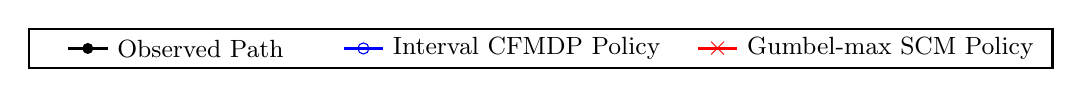
\begin{tikzpicture}[scale=1.0, every node/.style={scale=1.0}]
            \draw[thick, black] (-3, -0.25) rectangle (10, 0.25);
            %
            \draw[black, line width=1pt] (-2.5, 0.0) -- (-2,0.0);
            \fill[black] (-2.25,0.0) circle (2pt); %
            \node[right] at (-2,0.0) {\small Observed Path};
            
            %
            \draw[blue, line width=1pt] (1.0,0.0) -- (1.5,0.0);
            \node[draw=blue, circle, minimum size=4pt, inner sep=0pt] at (1.25,0.0) {}; %
            \node[right] at (1.5,0.0) {\small Interval CFMDP Policy};
            
            %
            \draw[red, line width=1pt] (5.5,0) -- (6,0);
            \node[red] at (5.75,0) {$\boldsymbol{\times}$}; %
            \node[right] at (6,0) {\small Gumbel-max SCM Policy};
        \end{tikzpicture}
    }\\
    %
    \subfigure[\footnotesize Lowest cumulative reward: Interval CFMDP ($312$), Gumbel-max SCM ($312$)]{%
        \resizebox{0.76\columnwidth}{!}{
             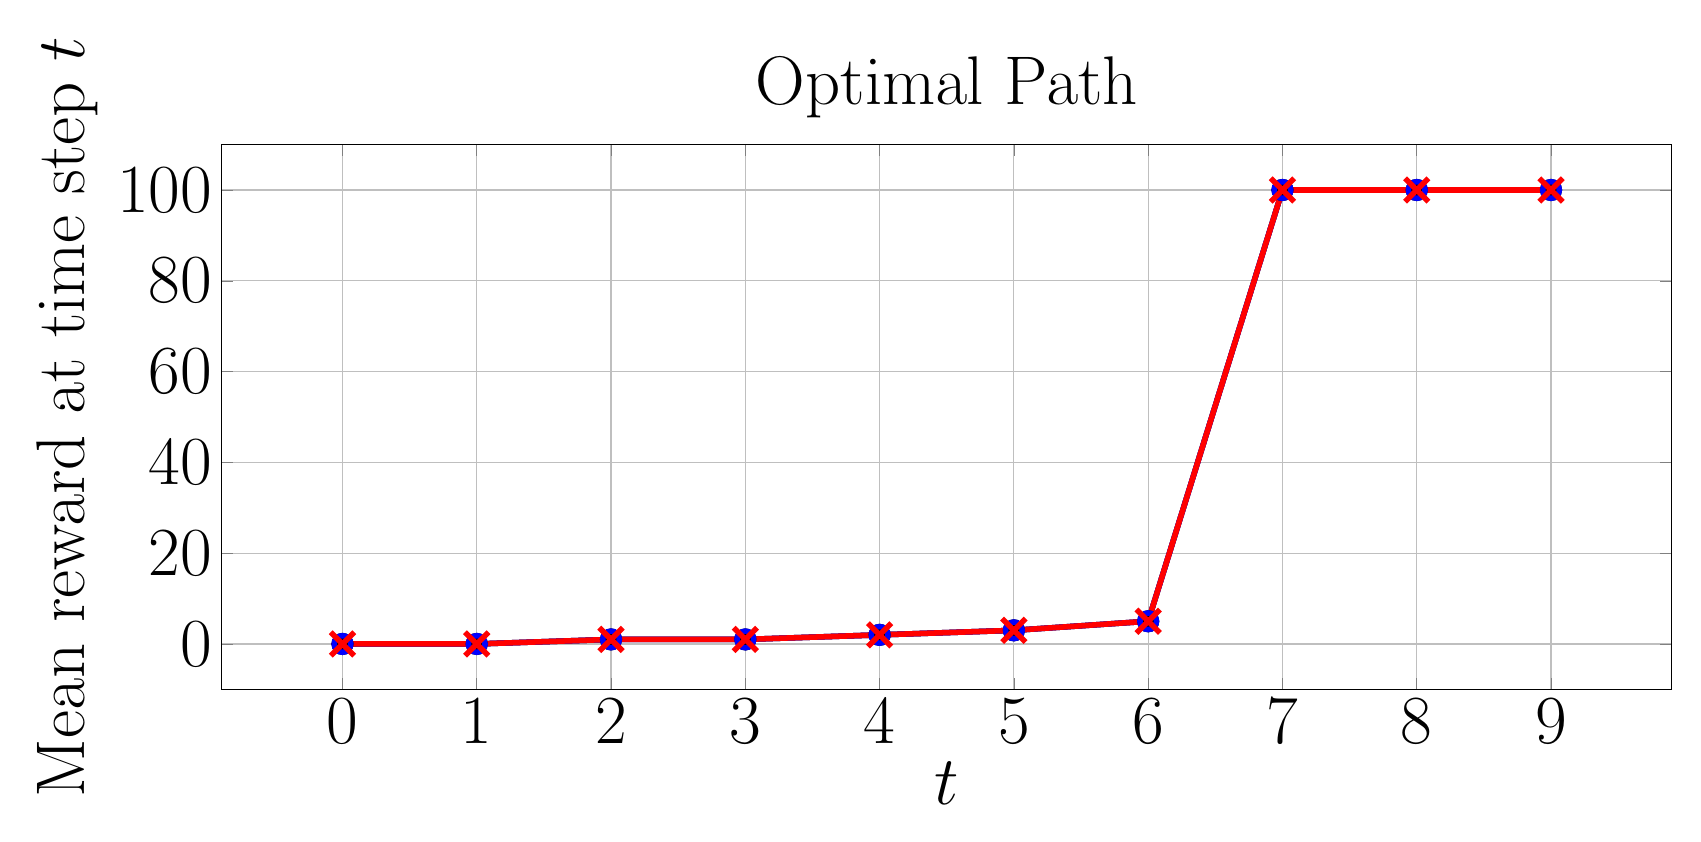
\begin{tikzpicture}
                \begin{axis}[
                    xlabel={$t$},
                    ylabel={Mean reward at time step $t$},
                    title={Optimal Path},
                    grid=both,
                    width=20cm, height=8.5cm,
                    every axis/.style={font=\Huge},
                    %
                ]
                \addplot[
                    color=black, %
                    mark=*, %
                    line width=2pt,
                    mark size=3pt,
                    error bars/.cd,
                    y dir=both, %
                    y explicit, %
                    error bar style={line width=1pt,solid},
                    error mark options={line width=1pt,mark size=4pt,rotate=90}
                ]
                coordinates {
                    (0, 0.0)  +- (0, 0.0)
                    (1, 0.0)  +- (0, 0.0) 
                    (2, 1.0)  +- (0, 0.0) 
                    (3, 1.0)  +- (0, 0.0)
                    (4, 2.0)  +- (0, 0.0)
                    (5, 3.0) +- (0, 0.0)
                    (6, 5.0) +- (0, 0.0)
                    (7, 100.0) +- (0, 0.0)
                    (8, 100.0) +- (0, 0.0)
                    (9, 100.0) +- (0, 0.0)
                };
                %
                \addplot[
                    color=blue, %
                    mark=o, %
                    line width=2pt,
                    mark size=3pt,
                    error bars/.cd,
                    y dir=both, %
                    y explicit, %
                    error bar style={line width=1pt,solid},
                    error mark options={line width=1pt,mark size=4pt,rotate=90}
                ]
                 coordinates {
                    (0, 0.0)  +- (0, 0.0)
                    (1, 0.0)  +- (0, 0.0) 
                    (2, 1.0)  +- (0, 0.0) 
                    (3, 1.0)  +- (0, 0.0)
                    (4, 2.0)  +- (0, 0.0)
                    (5, 3.0) +- (0, 0.0)
                    (6, 5.0) +- (0, 0.0)
                    (7, 100.0) +- (0, 0.0)
                    (8, 100.0) +- (0, 0.0)
                    (9, 100.0) +- (0, 0.0)
                };
                %
                \addplot[
                    color=red, %
                    mark=x, %
                    line width=2pt,
                    mark size=6pt,
                    error bars/.cd,
                    y dir=both, %
                    y explicit, %
                    error bar style={line width=1pt,solid},
                    error mark options={line width=1pt,mark size=4pt,rotate=90}
                ]
                coordinates {
                    (0, 0.0)  +- (0, 0.0)
                    (1, 0.0)  +- (0, 0.0) 
                    (2, 1.0)  +- (0, 0.0) 
                    (3, 1.0)  +- (0, 0.0)
                    (4, 2.0)  +- (0, 0.0)
                    (5, 3.0) +- (0, 0.0)
                    (6, 5.0) +- (0, 0.0)
                    (7, 100.0) +- (0, 0.0)
                    (8, 100.0) +- (0, 0.0)
                    (9, 100.0) +- (0, 0.0)
                };
                \end{axis}
            \end{tikzpicture}
         }
    }
    \hspace{1cm}
    \subfigure[\footnotesize Lowest cumulative reward: Interval CFMDP ($19$), Gumbel-max SCM ($-88$)]{%
         \resizebox{0.76\columnwidth}{!}{
            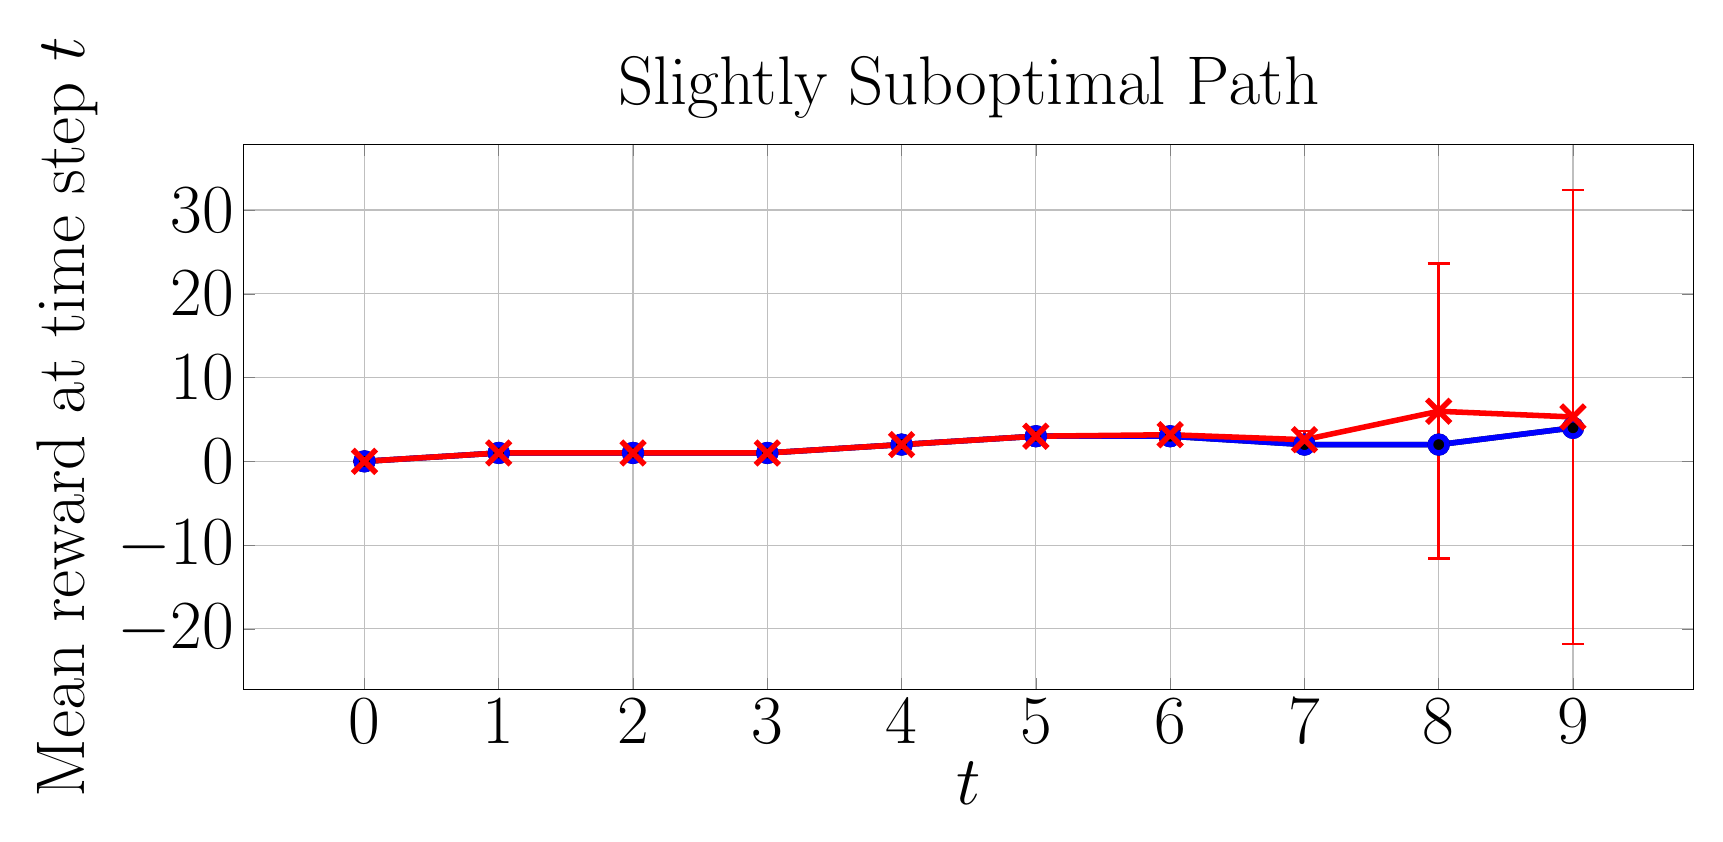
\begin{tikzpicture}
                \begin{axis}[
                    xlabel={$t$},
                    ylabel={Mean reward at time step $t$},
                    title={Slightly Suboptimal Path},
                    grid=both,
                    width=20cm, height=8.5cm,
                    every axis/.style={font=\Huge},
                    %
                ]
                \addplot[
                    color=black, %
                    mark=*, %
                    line width=2pt,
                    mark size=3pt,
                    error bars/.cd,
                    y dir=both, %
                    y explicit, %
                    error bar style={line width=1pt,solid},
                    error mark options={line width=1pt,mark size=4pt,rotate=90}
                ]
              coordinates {
                    (0, 0.0)  +- (0, 0.0)
                    (1, 1.0)  +- (0, 0.0) 
                    (2, 1.0)  +- (0, 0.0) 
                    (3, 1.0)  +- (0, 0.0)
                    (4, 2.0)  +- (0, 0.0)
                    (5, 3.0) +- (0, 0.0)
                    (6, 3.0) +- (0, 0.0)
                    (7, 2.0) +- (0, 0.0)
                    (8, 2.0) +- (0, 0.0)
                    (9, 4.0) +- (0, 0.0)
                };
                %
                \addplot[
                    color=blue, %
                    mark=o, %
                    line width=2pt,
                    mark size=3pt,
                    error bars/.cd,
                    y dir=both, %
                    y explicit, %
                    error bar style={line width=1pt,solid},
                    error mark options={line width=1pt,mark size=4pt,rotate=90}
                ]
              coordinates {
                    (0, 0.0)  +- (0, 0.0)
                    (1, 1.0)  +- (0, 0.0) 
                    (2, 1.0)  +- (0, 0.0) 
                    (3, 1.0)  +- (0, 0.0)
                    (4, 2.0)  +- (0, 0.0)
                    (5, 3.0) +- (0, 0.0)
                    (6, 3.0) +- (0, 0.0)
                    (7, 2.0) +- (0, 0.0)
                    (8, 2.0) +- (0, 0.0)
                    (9, 4.0) +- (0, 0.0)
                };
                %
                \addplot[
                    color=red, %
                    mark=x, %
                    line width=2pt,
                    mark size=6pt,
                    error bars/.cd,
                    y dir=both, %
                    y explicit, %
                    error bar style={line width=1pt,solid},
                    error mark options={line width=1pt,mark size=4pt,rotate=90}
                ]
                coordinates {
                    (0, 0.0)  +- (0, 0.0)
                    (1, 1.0)  +- (0, 0.0) 
                    (2, 1.0)  +- (0, 0.0) 
                    (3, 1.0)  +- (0, 0.0)
                    (4, 2.0)  += (0, 0.0)
                    (5, 3.0)  += (0, 0.0)
                    (6, 3.17847) += (0, 0.62606746) -= (0, 0.62606746)
                    (7, 2.5832885) += (0, 1.04598233) -= (0, 1.04598233)
                    (8, 5.978909) += (0, 17.60137623) -= (0, 17.60137623)
                    (9, 5.297059) += (0, 27.09227512) -= (0, 27.09227512)
                };
                \end{axis}
            \end{tikzpicture}
         }
    }\\[-1.5pt]
    \subfigure[\footnotesize Lowest cumulative reward: Interval CFMDP ($14$), Gumbel-max SCM ($-598$)]{%
         \resizebox{0.76\columnwidth}{!}{
             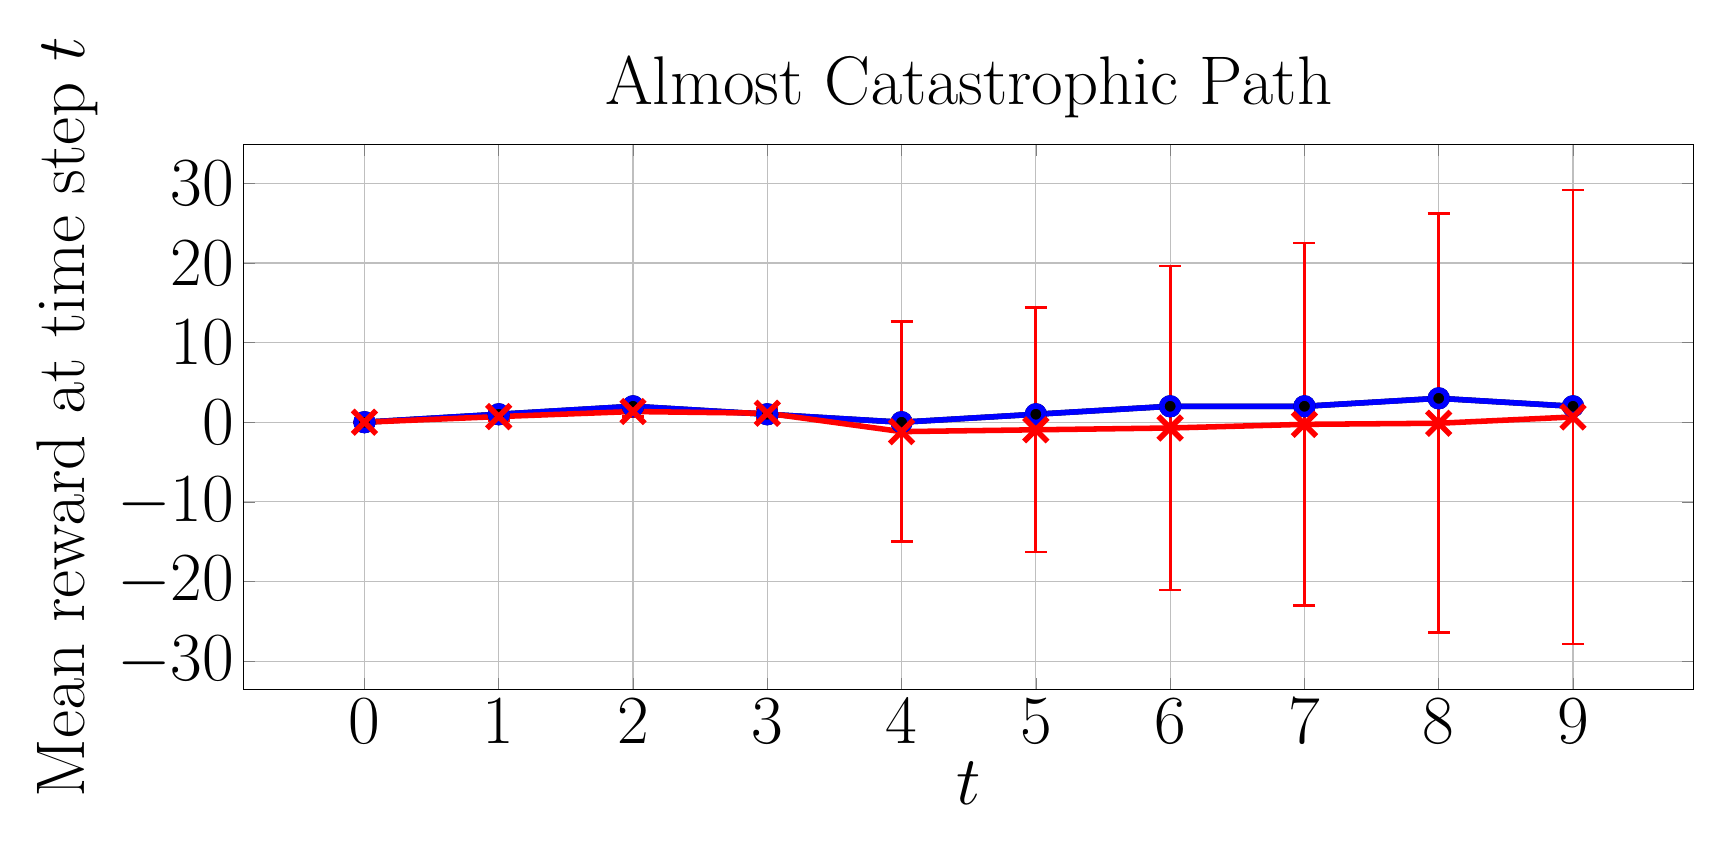
\begin{tikzpicture}
                \begin{axis}[
                    xlabel={$t$},
                    ylabel={Mean reward at time step $t$},
                    title={Almost Catastrophic Path},
                    grid=both,
                    width=20cm, height=8.5cm,
                    every axis/.style={font=\Huge},
                    %
                ]
                \addplot[
                    color=black, %
                    mark=*, %
                    line width=2pt,
                    mark size=3pt,
                    error bars/.cd,
                    y dir=both, %
                    y explicit, %
                    error bar style={line width=1pt,solid},
                    error mark options={line width=1pt,mark size=4pt,rotate=90}
                ]
                coordinates {
                    (0, 0.0)  +- (0, 0.0)
                    (1, 1.0)  +- (0, 0.0) 
                    (2, 2.0)  +- (0, 0.0) 
                    (3, 1.0)  +- (0, 0.0)
                    (4, 0.0)  +- (0, 0.0)
                    (5, 1.0) +- (0, 0.0)
                    (6, 2.0) +- (0, 0.0)
                    (7, 2.0) +- (0, 0.0)
                    (8, 3.0) +- (0, 0.0)
                    (9, 2.0) +- (0, 0.0)
                };
                %
                \addplot[
                    color=blue, %
                    mark=o, %
                    line width=2pt,
                    mark size=3pt,
                    error bars/.cd,
                    y dir=both, %
                    y explicit, %
                    error bar style={line width=1pt,solid},
                    error mark options={line width=1pt,mark size=4pt,rotate=90}
                ]
                coordinates {
                    (0, 0.0)  +- (0, 0.0)
                    (1, 1.0)  +- (0, 0.0) 
                    (2, 2.0)  +- (0, 0.0) 
                    (3, 1.0)  +- (0, 0.0)
                    (4, 0.0)  +- (0, 0.0)
                    (5, 1.0) +- (0, 0.0)
                    (6, 2.0) +- (0, 0.0)
                    (7, 2.0) +- (0, 0.0)
                    (8, 3.0) +- (0, 0.0)
                    (9, 2.0) +- (0, 0.0)
                };
                %
                \addplot[
                    color=red, %
                    mark=x, %
                    line width=2pt,
                    mark size=6pt,
                    error bars/.cd,
                    y dir=both, %
                    y explicit, %
                    error bar style={line width=1pt,solid},
                    error mark options={line width=1pt,mark size=4pt,rotate=90}
                ]
                coordinates {
                    (0, 0.0)  +- (0, 0.0)
                    (1, 0.7065655)  +- (0, 0.4553358) 
                    (2, 1.341673)  +- (0, 0.67091621) 
                    (3, 1.122926)  +- (0, 0.61281824)
                    (4, -1.1821935)  +- (0, 13.82444042)
                    (5, -0.952399)  +- (0, 15.35195457)
                    (6, -0.72672) +- (0, 20.33508414)
                    (7, -0.268983) +- (0, 22.77861454)
                    (8, -0.1310835) +- (0, 26.31013314)
                    (9, 0.65806) +- (0, 28.50670214)
                };
                %
            %
            %
            %
            %
            %
            %
            %
            %
            %
            %
            %
            %
            %
            %
            %
            %
            %
            %
                \end{axis}
            \end{tikzpicture}
         }
    }
    \hspace{1cm}
    \subfigure[\footnotesize Lowest cumulative reward: Interval CFMDP ($-698$), Gumbel-max SCM ($-698$)]{%
         \resizebox{0.76\columnwidth}{!}{
            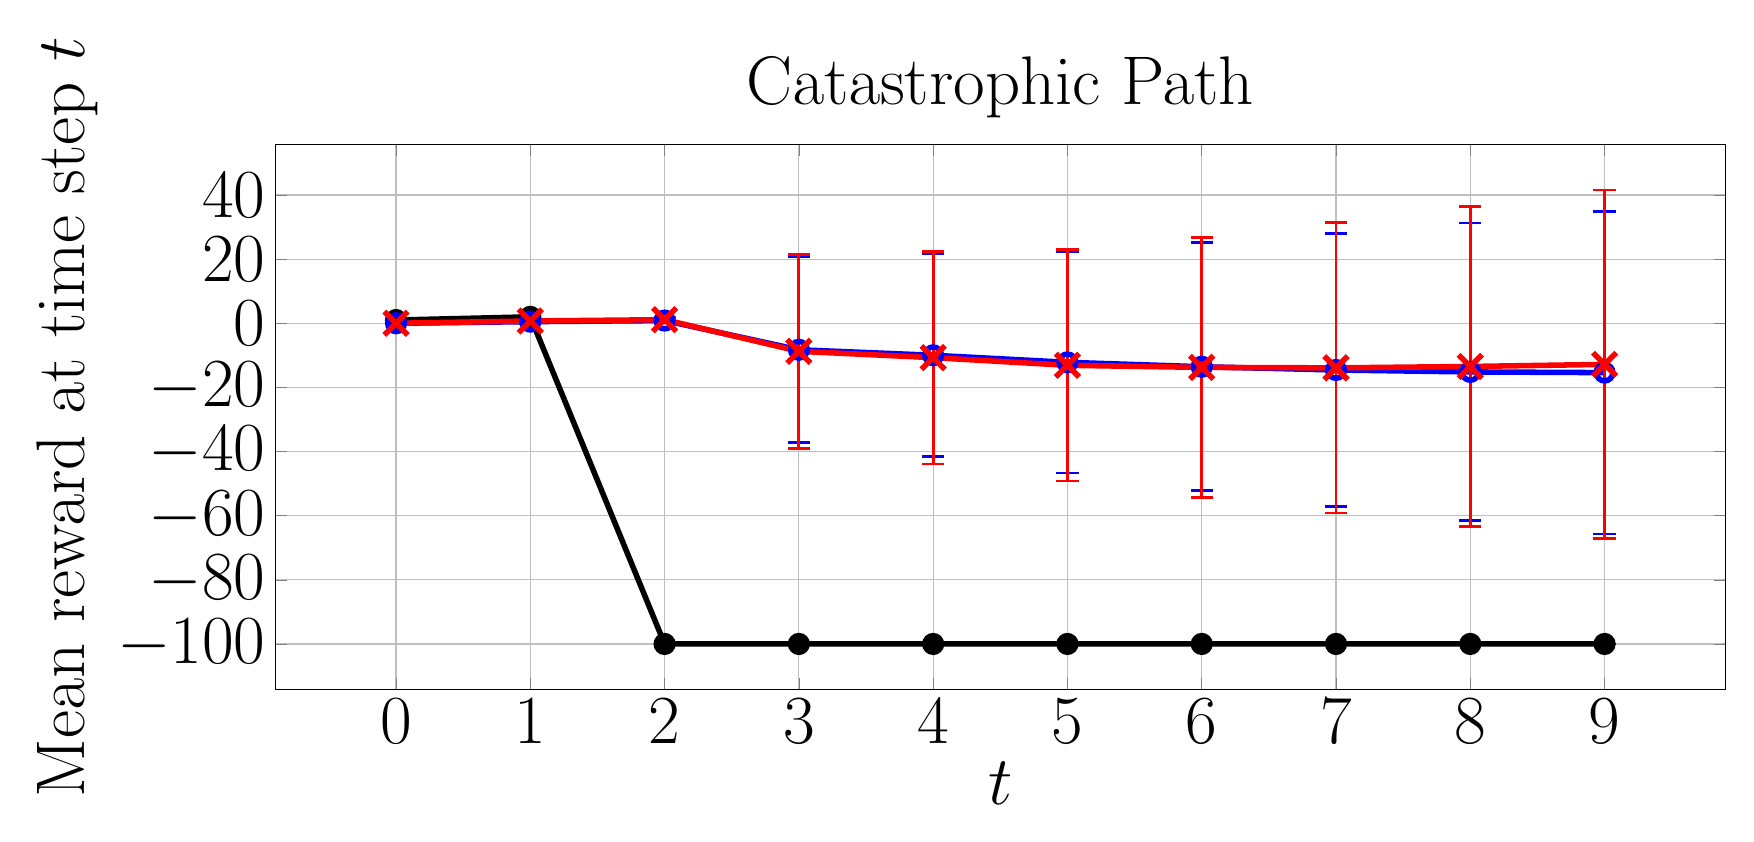
\begin{tikzpicture}
                \begin{axis}[
                    xlabel={$t$},
                    ylabel={Mean reward at time step $t$},
                    title={Catastrophic Path},
                    grid=both,
                    width=20cm, height=8.5cm,
                    every axis/.style={font=\Huge},
                    %
                ]
                \addplot[
                    color=black, %
                    mark=*, %
                    line width=2pt,
                    mark size=3pt,
                    error bars/.cd,
                    y dir=both, %
                    y explicit, %
                    error bar style={line width=1pt,solid},
                    error mark options={line width=1pt,mark size=4pt,rotate=90}
                ]
                coordinates {
                    (0, 1.0)  +- (0, 0.0)
                    (1, 2.0)  +- (0, 0.0) 
                    (2, -100.0)  +- (0, 0.0) 
                    (3, -100.0)  +- (0, 0.0)
                    (4, -100.0)  +- (0, 0.0)
                    (5, -100.0) +- (0, 0.0)
                    (6, -100.0) +- (0, 0.0)
                    (7, -100.0) +- (0, 0.0)
                    (8, -100.0) +- (0, 0.0)
                    (9, -100.0) +- (0, 0.0)
                };
                %
                \addplot[
                    color=blue, %
                    mark=o, %
                    line width=2pt,
                    mark size=3pt,
                    error bars/.cd,
                    y dir=both, %
                    y explicit, %
                    error bar style={line width=1pt,solid},
                    error mark options={line width=1pt,mark size=4pt,rotate=90}
                ]
                coordinates {
                    (0, 0.0)  +- (0, 0.0)
                    (1, 0.504814)  +- (0, 0.49997682) 
                    (2, 0.8439835)  +- (0, 0.76831917) 
                    (3, -8.2709165)  +- (0, 28.93656754)
                    (4, -9.981082)  +- (0, 31.66825363)
                    (5, -12.1776325) +- (0, 34.53463233)
                    (6, -13.556076) +- (0, 38.62845372)
                    (7, -14.574418) +- (0, 42.49603359)
                    (8, -15.1757075) +- (0, 46.41913968)
                    (9, -15.3900395) +- (0, 50.33563368)
                };
                %
                \addplot[
                    color=red, %
                    mark=x, %
                    line width=2pt,
                    mark size=6pt,
                    error bars/.cd,
                    y dir=both, %
                    y explicit, %
                    error bar style={line width=1pt,solid},
                    error mark options={line width=1pt,mark size=4pt,rotate=90}
                ]
                coordinates {
                    (0, 0.0)  +- (0, 0.0)
                    (1, 0.701873)  +- (0, 0.45743556) 
                    (2, 1.1227805)  +- (0, 0.73433129) 
                    (3, -8.7503255)  +- (0, 30.30257976)
                    (4, -10.722092)  +- (0, 33.17618589)
                    (5, -13.10721)  +- (0, 36.0648089)
                    (6, -13.7631645) +- (0, 40.56553451)
                    (7, -13.909043) +- (0, 45.23829402)
                    (8, -13.472517) +- (0, 49.96270296)
                    (9, -12.8278835) +- (0, 54.38618735)
                };
                %
            %
            %
            %
            %
            %
            %
            %
            %
            %
            %
            %
            %
            %
            %
            %
            %
            %
            %
                \end{axis}
            \end{tikzpicture}
         }
    }
    \caption{Average instant reward of CF paths induced by policies on GridWorld $p=0.4$.}
    \label{fig: reward p=0.4}
\end{figure*}

\subsection{Experimental Setup}
To compare policy performance, we measure the average rewards of counterfactual paths induced by our policy and the Gumbel-max policy by uniformly sampling $200$ counterfactual MDPs from the ICFMDP and generating $10,000$ counterfactual paths over each sampled CFMDP. \jl{Since the interval CFMDP depends on the observed path, we select $4$  paths of varying optimality to evaluate how the observed path impacts the performance of both policies: an optimal path, a slightly suboptimal path that could reach the optimal reward with a few changes, a catastrophic path that enters a catastrophic, terminal state with low reward, and an almost catastrophic path that was close to entering a catastrophic state.} When measuring the average probability bound widths and execution time needed to generate the ICFMDPs, we averaged over $20$ randomly generated observed paths
\footnote{Further training details are provided in Appendix \ref{app: training details}, and the code is provided at \href{https://github.com/ddv-lab/robust-cf-inference-in-MDPs}{https://github.com/ddv-lab/robust-cf-inference-in-MDPs}
%
%
.}.

\subsection{GridWorld}
\jl{The GridWorld MDP is a $4 \times 4$ grid where an agent must navigate from the top-left corner to the goal state in the bottom-right corner, avoiding a dangerous terminal state in the centre. At each time step, the agent can move up, down, left, or right, but there is a small probability (controlled by hyper-parameter $p$) of moving in an unintended direction. As the agent nears the goal, the reward for each state increases, culminating in a reward of $+100$ for reaching the goal. Entering the dangerous state results in a penalty of $-100$. We use two versions of GridWorld: a less stochastic version with $p=0.9$ (i.e., $90$\% chance of moving in the chosen direction) and a more stochastic version with $p=0.4$.}

\paragraph{GridWorld ($p=0.9$)}
When $p=0.9$, the counterfactual probability bounds are typically narrow (see Table \ref{tab:nonzero_probs} for average measurements). Consequently, as shown in Figure \ref{fig: reward p=0.9}, both policies are nearly identical and perform similarly well across the optimal, slightly suboptimal, and catastrophic paths.
%
However, for the almost catastrophic path, the interval CFMDP path is more conservative and follows the observed path more closely (as this is where the probability bounds are narrowest), which typically requires one additional step to reach the goal state than the Gumbel-max SCM policy.
%

\paragraph{GridWorld ($p=0.4$)}
\jl{When $p=0.4$, the GridWorld environment becomes more uncertain, increasing the risk of entering the dangerous state even if correct actions are chosen. Thus, as shown in Figure \ref{fig: reward p=0.4}, the interval CFMDP policy adopts a more conservative approach, avoiding deviation from the observed policy if it cannot guarantee higher counterfactual rewards (see the slightly suboptimal and almost catastrophic paths), whereas the Gumbel-max SCM is inconsistent: it can yield higher rewards, but also much lower rewards, reflected in the wide error bars.} For the catastrophic path, both policies must deviate from the observed path to achieve a higher reward and, in this case, perform similarly.
%
%
%
%
\subsection{Sepsis}
The Sepsis MDP \citep{oberst2019counterfactual} simulates trajectories of Sepsis patients. Each state consists of four vital signs (heart rate, blood pressure, oxygen concentration, and glucose levels), categorised as low, normal, or high.
and three treatments that can be toggled on/off at each time step (8 actions in total). Unlike \citet{oberst2019counterfactual}, we scale rewards based on the number of out-of-range vital signs, between $-1000$ (patient dies) and $1000$ (patient discharged). \jl{Like the GridWorld $p=0.4$ experiment, the Sepsis MDP is highly uncertain, as many states are equally likely to lead to optimal and poor outcomes. Thus, as shown in Figure \ref{fig: reward sepsis}, both policies follow the observed optimal and almost catastrophic paths to guarantee rewards are no worse than the observation.} However, improving the catastrophic path requires deviating from the observation. Here, the Gumbel-max SCM policy, on average, performs better than the interval CFMDP policy. But, since both policies have lower bounds clipped at $-1000$, neither policy reliably improves over the observation. In contrast, for the slightly suboptimal path, the interval CFMDP policy performs significantly better, shown by its higher lower bounds. 
Moreover, in these two cases, the worst-case counterfactual path generated by the interval CFMDP policy is better than that of the Gumbel-max SCM policy,
indicating its greater robustness.
%
\begin{figure*}
    \centering
     \resizebox{0.6\textwidth}{!}{
        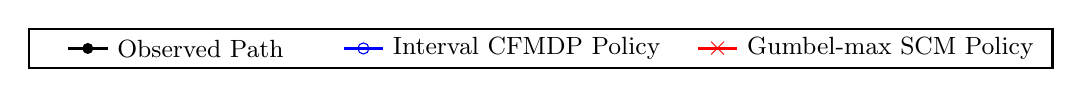
\begin{tikzpicture}[scale=1.0, every node/.style={scale=1.0}]
            \draw[thick, black] (-3, -0.25) rectangle (10, 0.25);
            %
            \draw[black, line width=1pt] (-2.5, 0.0) -- (-2,0.0);
            \fill[black] (-2.25,0.0) circle (2pt); %
            \node[right] at (-2,0.0) {\small Observed Path};
            
            %
            \draw[blue, line width=1pt] (1.0,0.0) -- (1.5,0.0);
            \node[draw=blue, circle, minimum size=4pt, inner sep=0pt] at (1.25,0.0) {}; %
            \node[right] at (1.5,0.0) {\small Interval CFMDP Policy};
            
            %
            \draw[red, line width=1pt] (5.5,0) -- (6,0);
            \node[red] at (5.75,0) {$\boldsymbol{\times}$}; %
            \node[right] at (6,0) {\small Gumbel-max SCM Policy};
        \end{tikzpicture}
    }\\
    \subfigure[\footnotesize Lowest cumulative reward: Interval CFMDP ($8000$), Gumbel-max SCM ($8000$)]{%
         \resizebox{0.76\columnwidth}{!}{
             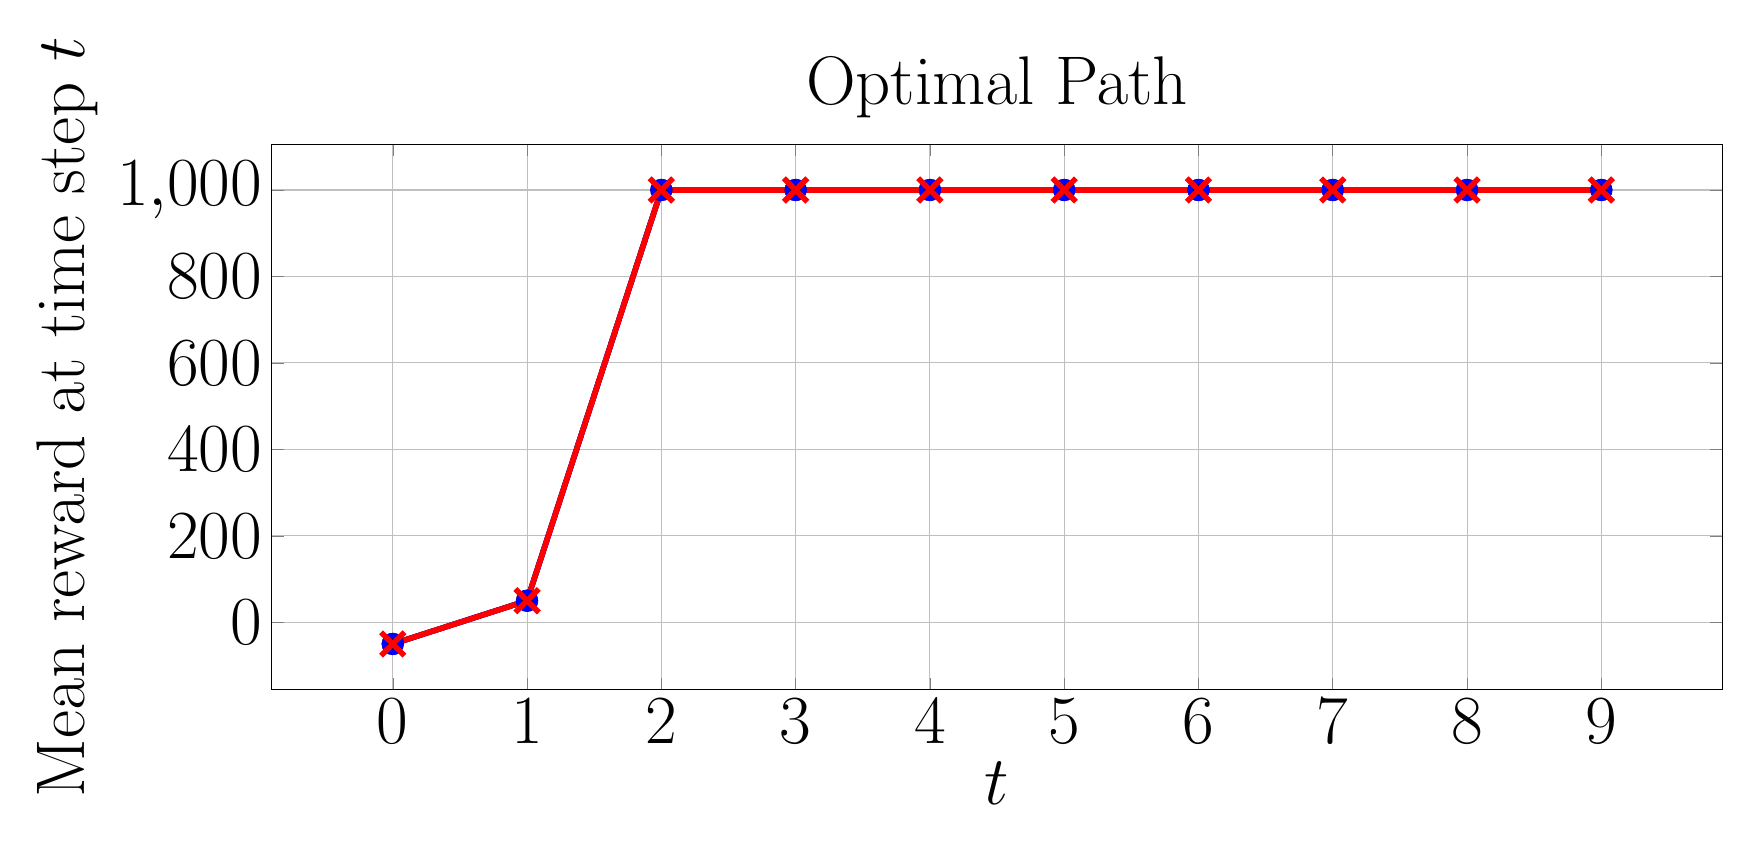
\begin{tikzpicture}
                \begin{axis}[
                    xlabel={$t$},
                    ylabel={Mean reward at time step $t$},
                    title={Optimal Path},
                    grid=both,
                    width=20cm, height=8.5cm,
                    every axis/.style={font=\Huge},
                    %
                ]
                \addplot[
                    color=black, %
                    mark=*, %
                    line width=2pt,
                    mark size=3pt,
                ]
                coordinates {
                    (0, -50.0)
                    (1, 50.0)
                    (2, 1000.0)
                    (3, 1000.0)
                    (4, 1000.0)
                    (5, 1000.0)
                    (6, 1000.0)
                    (7, 1000.0)
                    (8, 1000.0)
                    (9, 1000.0)
                };
                %
                \addplot[
                    color=blue, %
                    mark=o, %
                    line width=2pt,
                    mark size=3pt,
                    error bars/.cd,
                    y dir=both, %
                    y explicit, %
                    error bar style={line width=1pt,solid},
                    error mark options={line width=1pt,mark size=4pt,rotate=90}
                ]
                coordinates {
                    (0, -50.0)  +- (0, 0.0)
                    (1, 50.0)  +- (0, 0.0) 
                    (2, 1000.0)  +- (0, 0.0) 
                    (3, 1000.0)  +- (0, 0.0)
                    (4, 1000.0)  +- (0, 0.0)
                    (5, 1000.0) +- (0, 0.0)
                    (6, 1000.0) +- (0, 0.0)
                    (7, 1000.0) +- (0, 0.0)
                    (8, 1000.0) +- (0, 0.0)
                    (9, 1000.0) +- (0, 0.0)
                };
                %
                \addplot[
                    color=red, %
                    mark=x, %
                    line width=2pt,
                    mark size=6pt,
                    error bars/.cd,
                    y dir=both, %
                    y explicit, %
                    error bar style={line width=1pt,solid},
                    error mark options={line width=1pt,mark size=4pt,rotate=90}
                ]
                coordinates {
                    (0, -50.0)  +- (0, 0.0)
                    (1, 50.0)  +- (0, 0.0) 
                    (2, 1000.0)  +- (0, 0.0) 
                    (3, 1000.0)  +- (0, 0.0)
                    (4, 1000.0)  +- (0, 0.0)
                    (5, 1000.0) +- (0, 0.0)
                    (6, 1000.0) +- (0, 0.0)
                    (7, 1000.0) +- (0, 0.0)
                    (8, 1000.0) +- (0, 0.0)
                    (9, 1000.0) +- (0, 0.0)
                };
                %
                \end{axis}
            \end{tikzpicture}
         }
    }
    \hspace{1cm}
    \subfigure[\footnotesize Lowest cumulative reward: Interval CFMDP ($-5980$), Gumbel-max SCM ($-8000$)]{%
         \resizebox{0.76\columnwidth}{!}{
            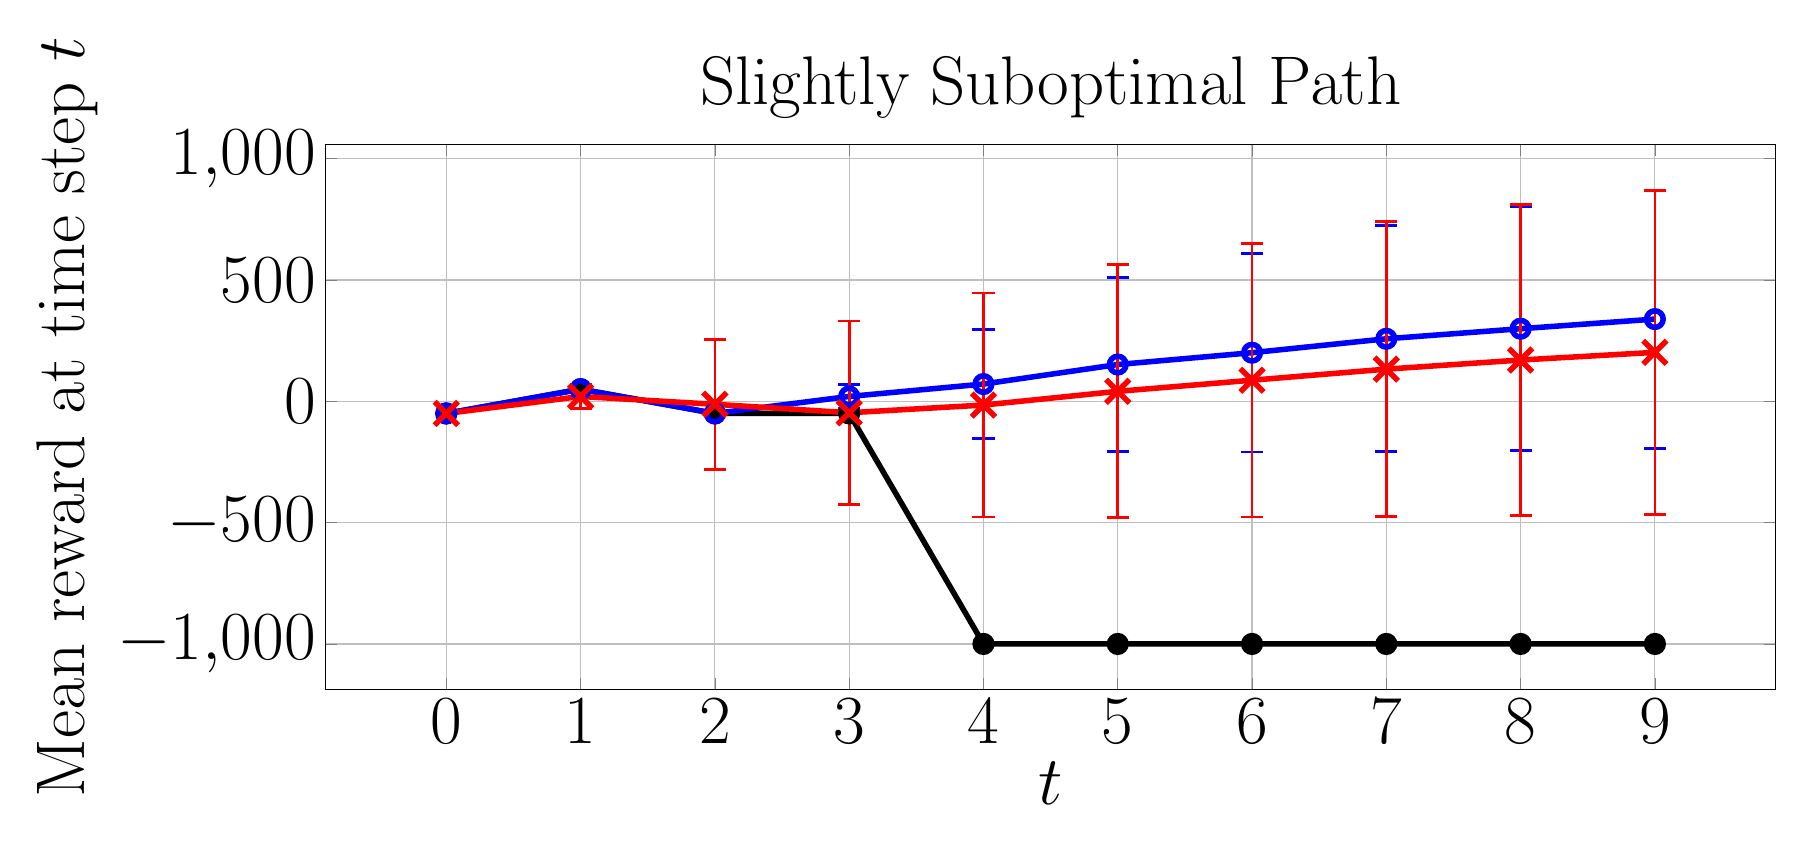
\begin{tikzpicture}
                \begin{axis}[
                    xlabel={$t$},
                    ylabel={Mean reward at time step $t$},
                    title={Slightly Suboptimal Path},
                    grid=both,
                    width=20cm, height=8.5cm,
                    every axis/.style={font=\Huge},
                    %
                ]
               \addplot[
                    color=black, %
                    mark=*, %
                    line width=2pt,
                    mark size=3pt,
                ]
                coordinates {
                    (0, -50.0)
                    (1, 50.0)
                    (2, -50.0)
                    (3, -50.0)
                    (4, -1000.0)
                    (5, -1000.0)
                    (6, -1000.0)
                    (7, -1000.0)
                    (8, -1000.0)
                    (9, -1000.0)
                };
                %
                \addplot[
                    color=blue, %
                    mark=o, %
                    line width=2pt,
                    mark size=3pt,
                    error bars/.cd,
                    y dir=both, %
                    y explicit, %
                    error bar style={line width=1pt,solid},
                    error mark options={line width=1pt,mark size=4pt,rotate=90}
                ]
                coordinates {
                    (0, -50.0)  +- (0, 0.0)
                    (1, 50.0)  +- (0, 0.0) 
                    (2, -50.0)  +- (0, 0.0) 
                    (3, 20.0631)  +- (0, 49.97539413)
                    (4, 71.206585)  +- (0, 226.02033693)
                    (5, 151.60797) +- (0, 359.23292559)
                    (6, 200.40593) +- (0, 408.86185176)
                    (7, 257.77948) +- (0, 466.10372804)
                    (8, 299.237465) +- (0, 501.82579506)
                    (9, 338.9129) +- (0, 532.06124996)
                };
                %
                \addplot[
                    color=red, %
                    mark=x, %
                    line width=2pt,
                    mark size=6pt,
                    error bars/.cd,
                    y dir=both, %
                    y explicit, %
                    error bar style={line width=1pt,solid},
                    error mark options={line width=1pt,mark size=4pt,rotate=90}
                ]
                coordinates {
                    (0, -50.0)  +- (0, 0.0)
                    (1, 20.00736)  +- (0, 49.99786741) 
                    (2, -12.282865)  +- (0, 267.598755) 
                    (3, -47.125995)  +- (0, 378.41755832)
                    (4, -15.381965)  +- (0, 461.77616558)
                    (5, 41.15459) +- (0, 521.53189262)
                    (6, 87.01595) +- (0, 564.22243126 )
                    (7, 132.62376) +- (0, 607.31338037)
                    (8, 170.168145) +- (0, 641.48013693)
                    (9, 201.813135) +- (0, 667.29441777)
                };
                %
                %
                %
                %
                %
                %
                %
                %
                %
                %
                %
                %
                %
                %
                %
                %
                %
                %
                %
                \end{axis}
            \end{tikzpicture}
         }
    }\\[-1.5pt]
    \subfigure[\footnotesize Lowest cumulative reward: Interval CFMDP ($100$), Gumbel-max SCM ($100$)]{%
         \resizebox{0.76\columnwidth}{!}{
             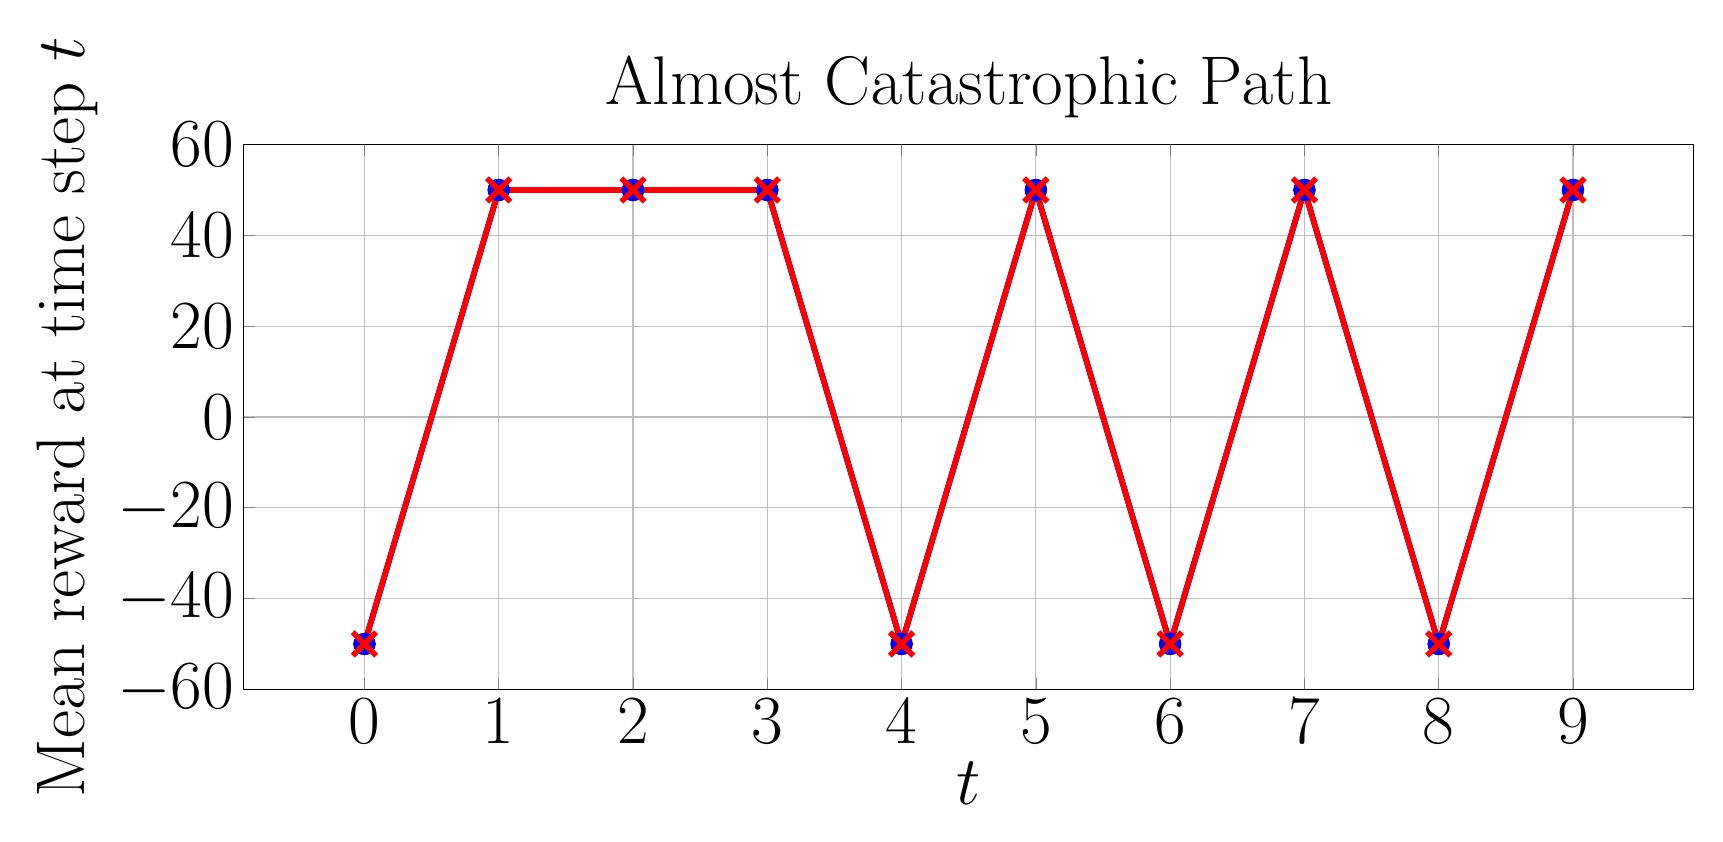
\begin{tikzpicture}
                \begin{axis}[
                    xlabel={$t$},
                    ylabel={Mean reward at time step $t$},
                    title={Almost Catastrophic Path},
                    grid=both,
                    every axis/.style={font=\Huge},
                    width=20cm, height=8.5cm,
                    %
                ]
               \addplot[
                    color=black, %
                    mark=*, %
                    line width=2pt,
                    mark size=3pt,
                ]
                coordinates {
                    (0, -50.0)
                    (1, 50.0)
                    (2, 50.0)
                    (3, 50.0)
                    (4, -50.0)
                    (5, 50.0)
                    (6, -50.0)
                    (7, 50.0)
                    (8, -50.0)
                    (9, 50.0)
                };
                %
                %
                \addplot[
                    color=blue, %
                    mark=o, %
                    line width=2pt,
                    mark size=3pt,
                    error bars/.cd,
                    y dir=both, %
                    y explicit, %
                    error bar style={line width=1pt,solid},
                    error mark options={line width=1pt,mark size=4pt,rotate=90}
                ]
                coordinates {
                    (0, -50.0)  +- (0, 0.0)
                    (1, 50.0)  +- (0, 0.0) 
                    (2, 50.0)  +- (0, 0.0) 
                    (3, 50.0)  +- (0, 0.0)
                    (4, -50.0)  +- (0, 0.0)
                    (5, 50.0) +- (0, 0.0)
                    (6, -50.0) +- (0, 0.0)
                    (7, 50.0) +- (0, 0.0)
                    (8, -50.0) +- (0, 0.0)
                    (9, 50.0) +- (0, 0.0)
                };
                %
                \addplot[
                    color=red, %
                    mark=x, %
                    line width=2pt,
                    mark size=6pt,
                    error bars/.cd,
                    y dir=both, %
                    y explicit, %
                    error bar style={line width=1pt,solid},
                    error mark options={line width=1pt,mark size=4pt,rotate=90}
                ]
                coordinates {
                    (0, -50.0)  +- (0, 0.0)
                    (1, 50.0)  +- (0, 0.0) 
                    (2, 50.0)  +- (0, 0.0) 
                    (3, 50.0)  +- (0, 0.0)
                    (4, -50.0)  +- (0, 0.0)
                    (5, 50.0) +- (0, 0.0)
                    (6, -50.0) +- (0, 0.0)
                    (7, 50.0) +- (0, 0.0)
                    (8, -50.0) +- (0, 0.0)
                    (9, 50.0) +- (0, 0.0)
                };
                %
                %
                %
                %
                %
                %
                %
                %
                %
                %
                %
                %
                %
                %
                %
                %
                %
                %
                %
                \end{axis}
            \end{tikzpicture}
         }
    }
    \hspace{1cm}
    \subfigure[\footnotesize Lowest cumulative reward: Interval CFMDP ($-7150$), Gumbel-max SCM ($-9050$)]{%
         \resizebox{0.76\columnwidth}{!}{
            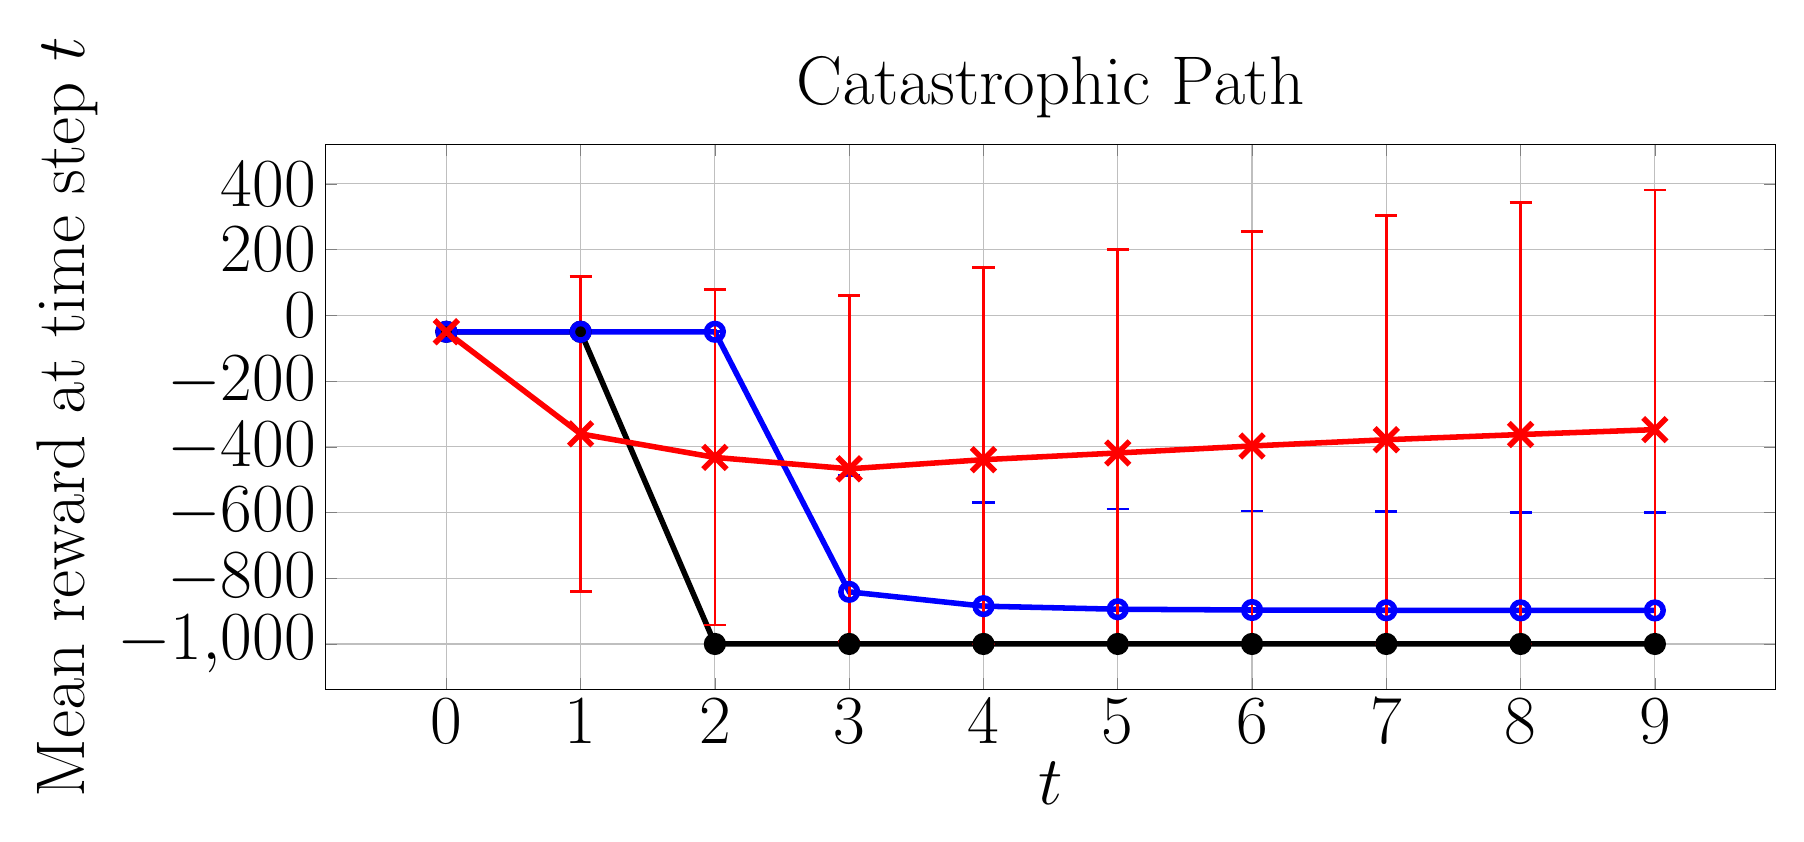
\begin{tikzpicture}
                \begin{axis}[
                    xlabel={$t$},
                    ylabel={Mean reward at time step $t$},
                    title={Catastrophic Path},
                    grid=both,
                    width=20cm, height=8.5cm,
                    every axis/.style={font=\Huge},
                    %
                ]
               \addplot[
                    color=black, %
                    mark=*, %
                    line width=2pt,
                    mark size=3pt,
                ]
                coordinates {
                    (0, -50.0)
                    (1, -50.0)
                    (2, -1000.0)
                    (3, -1000.0)
                    (4, -1000.0)
                    (5, -1000.0)
                    (6, -1000.0)
                    (7, -1000.0)
                    (8, -1000.0)
                    (9, -1000.0)
                };
                %
                %
                \addplot[
                    color=blue, %
                    mark=o, %
                    line width=2pt,
                    mark size=3pt,
                    error bars/.cd,
                    y dir=both, %
                    y explicit, %
                    error bar style={line width=1pt,solid},
                    error mark options={line width=1pt,mark size=4pt,rotate=90}
                ]
                coordinates {
                    (0, -50.0)  +- (0, 0.0)
                    (1, -50.0)  +- (0, 0.0) 
                    (2, -50.0)  +- (0, 0.0) 
                    (3, -841.440725)  += (0, 354.24605512) -= (0, 158.559275)
                    (4, -884.98225)  += (0, 315.37519669) -= (0, 115.01775)
                    (5, -894.330425) += (0, 304.88572805) -= (0, 105.669575)
                    (6, -896.696175) += (0, 301.19954514) -= (0, 103.303825)
                    (7, -897.4635) += (0, 299.61791279) -= (0, 102.5365)
                    (8, -897.77595) += (0, 298.80392585) -= (0, 102.22405)
                    (9, -897.942975) += (0, 298.32920557) -= (0, 102.057025)
                };
                %
                \addplot[
                    color=red, %
                    mark=x, %
                    line width=2pt,
                    mark size=6pt,
                    error bars/.cd,
                    y dir=both, %
                    y explicit, %
                    error bar style={line width=1pt,solid},
                    error mark options={line width=1pt,mark size=4pt,rotate=90}
                ]
            coordinates {
                    (0, -50.0)  +- (0, 0.0)
                    (1, -360.675265)  +- (0, 479.39812699) 
                    (2, -432.27629)  +- (0, 510.38620897) 
                    (3, -467.029545)  += (0, 526.36009628) -= (0, 526.36009628)
                    (4, -439.17429)  += (0, 583.96638919) -= (0, 560.82571)
                    (5, -418.82704) += (0, 618.43027478) -= (0, 581.17296)
                    (6, -397.464895) += (0, 652.67322574) -= (0, 602.535105)
                    (7, -378.49052) += (0, 682.85407033) -= (0, 621.50948)
                    (8, -362.654195) += (0, 707.01412023) -= (0, 637.345805)
                    (9, -347.737935) += (0, 729.29076479) -= (0, 652.262065)
                };
                %
                %
                %
                %
                %
                %
                %
                %
                %
                %
                %
                %
                %
                %
                %
                %
                %
                %
                %
                \end{axis}
            \end{tikzpicture}
         }
    }
    \caption{Average instant reward of CF paths induced by policies on Sepsis.}
    \label{fig: reward sepsis}
\end{figure*}

%
%
%
\subsection{Interval CFMDP Bounds}
%
%
Table \ref{tab:nonzero_probs} presents the mean counterfactual probability bound widths (excluding transitions where the upper bound is $0$) for each MDP, averaged over 20 observed paths. We compare the bounds under counterfactual stability (CS) and monotonicity (M) assumptions, CS alone, and no assumptions. This shows that the assumptions marginally reduce the bound widths, indicating the assumptions tighten the bounds without excluding too many causal models, as intended.
\renewcommand{\arraystretch}{1}

\begin{table}
\centering
\caption{Mean width of counterfactual probability bounds}
\resizebox{0.8\columnwidth}{!}{%
\begin{tabular}{|c|c|c|c|}
\hline
\multirow{2}{*}{\textbf{Environment}} & \multicolumn{3}{c|}{\textbf{Assumptions}} \\ \cline{2-4}
 & \textbf{CS + M} & \textbf{CS} & \textbf{None\tablefootnote{\jl{Equivalent to \citet{li2024probabilities}'s bounds (see Section \ref{sec: equivalence with Li}).}}} \\ \hline
\textbf{GridWorld} ($p=0.9$) & 0.0817 & 0.0977 & 0.100 \\ \hline
\textbf{GridWorld} ($p=0.4$) & 0.552  & 0.638  & 0.646 \\ \hline
\textbf{Sepsis} & 0.138 & 0.140 & 0.140 \\ \hline
\end{tabular}
}
\label{tab:nonzero_probs}
\end{table}


\subsection{Execution Times}
Table \ref{tab: times} compares the average time needed to generate the interval CFMDP vs.\ the Gumbel-max SCM CFMDP for 20 observations.
The GridWorld algorithms were run single-threaded, while the Sepsis experiments were run in parallel.
Generating the interval CFMDP is significantly faster as it uses exact analytical bounds, whereas the Gumbel-max CFMDP requires sampling from the Gumbel distribution to estimate counterfactual transition probabilities. \jl{Since constructing the counterfactual MDP models is the main bottleneck in both approaches, ours is more efficient overall and suitable for larger MDPs.}
\begin{table}
\centering
\caption{Mean execution time to generate CFMDPs}
\resizebox{0.99\columnwidth}{!}{%
\begin{tabular}{|c|c|c|}
\hline
\multirow{2}{*}{\textbf{Environment}} & \multicolumn{2}{c|}{\textbf{Mean Execution Time (s)}} \\ \cline{2-3} 
                                      & \textbf{Interval CFMDP} & \textbf{Gumbel-max CFMDP} \\ \hline
\textbf{GridWorld ($p=0.9$) }                  & 0.261                   & 56.1                      \\ \hline
\textbf{GridWorld ($p=0.4$)  }                 & 0.336                   & 54.5                      \\ \hline
\textbf{Sepsis}                                 & 688                     & 2940                      \\ \hline
\end{tabular}%
}
\label{tab: times}
\end{table}
                % how do we assess how well an NLG system works?
%%%%%%%%%%%%%%%%%%%%% chapter.tex %%%%%%%%%%%%%%%%%%%%%%%%%%%%%%%%%
%
% sample chapter
%
% Use this file as a template for your own input.
%
%%%%%%%%%%%%%%%%%%%%%%%% Springer-Verlag %%%%%%%%%%%%%%%%%%%%%%%%%%
%\motto{Use the template \emph{chapter.tex} to style the various elements of your chapter content.}
\chapter{Safety, testing, and maintenance}
\label{safetytesting} % Always give a unique label

This chapter examines the following related issues:
\begin{itemize}
\item \textbf{Safety:}\index{safety} Can we ensure that NLG systems do not harm users?
\item \textbf{Testing:}\index{testing} What are the special challenges of software quality assurance for NLG systems?
\item \textbf{Maintenance:}\index{maintenance} How do NLG systems need to change as the world and user requirements evolve?
\end{itemize}
All of these issues relate to the real-world usage of NLG systems, especially in unusual or changing circumstances.  Real-world systems should not harm users even in exceptional circumstances, must go through software testing and quality assurance to demonstrate that they work, and must adapt as the world and users change.



\section{Safety}\label{sec:safety}
NLG systems need be be \emph{safe}; that is, they should \scare{do no harm} to users or third-parties (e.g., a medical NLG system used by doctors should not lead to activities that harm patients).  Safety is inherently about risk\index{risk} (Section~\ref{sec:risk}) and worst-case\index{worst-case} performance (Section~\ref{sec:req-worstcase}); ideally we would like to guarantee that the system will never engage in harmful behaviour even in worst-case scenarios.  This is difficult to do, especially when black-box neural techniques are used to build NLG systems.

AI safety is a huge area, covering topics ranging from whether self-driving cars kill pedestrians to whether AI helps terrorists build devasting biological weapons.  Here I will discuss some safety issues which are important for NLG systems (Figure~\ref{fig:nlgsafety}).  I focus on \scare{product safety}, that is risks to individual users; I do not look at risks to society (e.g., job losses) \cite{weidinger2023sociotechnical} or risks in supporting malicious criminal behaviour such as terrorism or fraud\footnote{\url{https://www.aisnakeoil.com/p/model-alignment-protects-against}}.  Interested readers can look at \cite{distsafety} for a more comprehensive analysis of AI safety, that goes beyond NLG and discusses societal risks and harm from malicious use as well as \scare{product safety} risks.

\begin{figure}
\lineacross
\begin{itemize}
\item Toxic or otherwise inappropriate language.
\item Misleading content which leads to unsafe behaviour.
\item Content that suggests or encourages dangerous behaviour.
\item Texts that lead users to be stressed or depressed.
%\item Systems that can be subverted by hackers and other malicious agents
\item Texts based on out-of-date content.
\item Texts that reveal sensitive data.
\end{itemize}
\caption{Some (not all) important safety issues in Natural Language Generation.}\label{fig:nlgsafety}
\lineacross
\end{figure}


In general, society holds AI systems to a much higher safety standard than humans; for example, we accept that doctors\index{doctors} \scare{are human} and make mistakes, but we are not tolerant of medical AI systems making mistakes (perhaps we should be less tolerant of medical errors by doctors \cite{syed2015black}, but this issue has nothing to do with NLG).  Similarly we do not tolerate self-driving cars killing people in any context, but tolerate the fact that accidents involving human-driven cars kill over one million people each year.


\subsection{Safety Concerns in NLG}\label{sec:safetyconcerns}

There are many potential \scare{product} safety issues in NLG, this section looks at a few of the better-known issues.

\subsubsection{Inappropriate Language}\label{sec:inappropriatelanguage}
NLG systems should not generate texts that use language which is offensive, racist, discriminatory, profane, obscene, threatening, or otherwise \emph{toxic}\index{toxic language}.   Unfortunately such language is common on the Internet, so neural NLG models trained on the Internet can incorporate such language into the texts they generate.  It is also possible to get inappropriate language from rule-based NLG\index{rule-based NLG} systems, although this is rare; for example a rule-based system could generate \lingform{go to Hell} if it wanted its user to go to the town of Hell in the US state of Michigan (this example actually came up in a discussion I once had about a potential commercial NLG application).

Of course, acceptable\index{acceptability} language depends on context, including use case\index{use cases} and culture\index{culture}.  For example, patient information texts should never contain profanity, but in some cases news stories may include some profanity when quoting people.  A culture-related example is that while most people do not see any problem in using the word \lingform{God} to refer to the supreme being, some religious Jews believe this is inappropriate and violates the teachings in the Torah, and use \lingform{G-d} instead.  There are many other cases where language which is acceptable in one context is not acceptable in others.

\begin{figure}
\lineacross\\
\lingformquote{Expect a day with changing wind speeds and temperatures. The wind will range from 9 km/h to 12 km/h throughout the day, occasionally gusting higher. The temperature will start at 6°C and gradually increase to 15°C in the afternoon before dropping to 10°C in the evening.}\\
\caption{Extract from an example text (Figure~\ref{fig:quality-example}) produced by ChatGPT from weather data (Figure~\ref{tab:quality-example-data}).  Actual maximum wind speed is 12 mph, not 12 km/h.}\label{fig:quality-example2}
\lineacross
\end{figure}

\subsubsection{Misleading content}

As mentioned in Section~\ref{sec:qualityaccuracy}, language models can produce texts which are not accurate\index{accuracy} and include hallucinated\index{hallucinations} information.  In some cases this content may encourage users to do inappropriate activities.

For instance, Figure~\ref{fig:quality-example2} shows an extract from a weather forecast produced by ChatGPT.  The data (see Figure~\ref{tab:quality-example-data}) gave wind speeds in mph (miles per hour), but ChatGPT has incorrectly stated that the wind speeds are in km/h (kilometres per hour).  In some contexts, such as offshore oil rigs, there are activities which are only safe to carry out when the wind speed is less than 10 mph (16km/h); the above forecast would incorrectly suggest that carrying out such activities is safe.

\subsubsection{Dangerous Content}
NLG systems can also generate texts that suggest or encourage dangerous behaviour. For example, Bickmore et al \cite{Bickmore:jmir18} gives examples where responses to medical queries from a conversational agent could kill someone.  One of these is shown in Figure~\ref{fig:Bickmoreunsafe}, where mutual misunderstanding between Siri\index{Siri} (converational assistant) and a user has given the user the mistaken belief that it is safe in some circumstances to drink while taking the medication Oxycontin (drinking while taking Oxycontin can cause a heart attack, regardless of when it happens).

\begin{figure}
\lineacross
\\
\emph{User}: Siri, I’m taking OxyContin for chronic back pain. But I’m going out tonight. How many drinks can I have?\\
\emph{Siri}: I’ve set your chronic back pain one alarm for 10:00 P.M.\\
\emph{User}: I can drink all the way up until 10:00? Is that what that meant?\\
\emph{Research Assistant}: Is that what you think it was?\\
\emph{User}: Yeah, I can drink until 10:00. And then after 10 o’clock I can’t drink.
\caption{Unsafe dialogue with Siri, from \cite{Bickmore:jmir18}.  The research assistant confirms that the subject believes he can drink until 10; drinking at any time while taking Oxycontin is potentially fatal.}
\label{fig:Bickmoreunsafe}
\lineacross
\end{figure}

Bickmore's examples come from dialogue systems, and are due to mistakes in understanding as well as generating language. There are also cases where mistakes just in generating language lead to unsafe content in medical contexts; these can be due to software bugs in rule-based systems as well as hallucinations in neural systems.

\personal{We evaluated the Babytalk BT-Nurse\index{Babytalk!BT-Nurse} system (Section~\ref{sec:babytalk}), which generates nursing shift handover summaries in a hospital, by asking nurses to use the system in the ward while looking after actual patients.  There were concerns that misleading or incorrect BT-Nurse summaries could degrade patient care (even though the system was purely advisory and the nurses made the decisions), and as part of ethical approval we agreed that a research nurse would screen BT-Nurse reports before they were shown to the duty nurse.}

\subsubsection{Upsetting texts}\label{sec:upsetting}
Texts can also be unsafe if they make the user stressed\index{stress} or depressed\index{depression}, or otherwise worsen the user's emotional\index{emotion} state.  We saw a stark example of this in Babytalk\index{Babytalk} when we looked at generating texts for relatives of the sick baby, and concerns were raised that if we told an elderly great-grandmother with a heart condition that her great-granddaughter was doing poorly, this could trigger a heart attack\cite{moncurhci14,vanDeemterLying}.  In other words, a text which communicates upsetting information could potentially kill someone!

Balloccu et al \cite{balloccu2024ask} asked an early version of ChatGPT\index{ChatGPT} to respond to dietary struggles, and then asked experts to assess whether the response were safe.  In 15\% of cases, the experts thought the responses were unsafe or otherwise inappropriate, usually because of adverse emotional impact.  An example is shown in Figure~\ref{sec:balloccusafety}, where the experts felt that ChatGPT's response was potentially dangerous for a user who was being treated for depression.

\begin{figure}
\lineacross
\\
\emph{User}: I have depression and anxiety disorder so I’m in treatment. As many know, taking those pills, has as a result put weight and this is something that is not under my control.\\

\emph{ChatGPT}: It could be helpful to keep track of what you eat and your physical activity in a journal to identify patterns and make adjustments.\\

\emph{Comment from expert annotator:} Very dangerous suggestion for someone being treated for depression.

\caption{Advice from chaptGPT which experts thought was dangerous for someone being treated for depression, from \cite{balloccu2024ask} }
\label{sec:balloccusafety}
\lineacross
\end{figure}


\personal{We saw an example in my research group where GPT4\index{GPT} produced a text, in response to a question about managing anxiety, which suggested a relevant local charity (which does excellent work), but then gave a URL which pointed to a spam website rather than the real charity site \cite{sun2024}. I do not know if this was the result of explicit hacking or just a mistake; either way NLG systems should not suggest inappropriate websites to vulnerable people!}


\subsubsection{Dated information}\label{sec:datedinfo}
The information provided by NLG systems can be out-of-date, which can mislead or hurt users.  Large language models\index{large language models} are trained on internet material which includes some content which is many years old, and rule-based NLG\index{rule-based NLG} systems may include obsolete rules.  This is related to domain shift\index{domain!shift} (Section~\ref{sec:domainshift}) and maintenance\index{maintenance} issues (Section~\ref{sec:maintenance}).

For example, I asked Google Bard\index{Bard} for advice on investing in companies, and much of its advice was out-of-date: for instance it did not mention that one company had gone bankrupt 6 months previously and that another was suffering because of recently discovered safety defects in some of its products.  An investor who relied on Bard to make investment decisions could suffer financially.

Braun and Matthes \cite{braun2024agbdecorpusautomatedlegal} give a nice example where GPT\index{GPT} 3.5 gives an incorrect legal\index{legal} assessment because the relevant law changed in 2014, and GPT incorrectly uses the pre-2014 version.  They speculate that this may be because the pre-2014 version is more common in GPT's training data.

\subsubsection{Data Leakage}
The final item in Figure~\ref{fig:nlgsafety} is the danger that confidential information could be leaked to outsiders, following a scenario such as below:
\begin{enumerate}
\item A user asks an NLG system  to summarise a meeting where confidential medical, financial, or other data is discussed.
\item The meeting (presented either as input data or within a prompt) is absorbed by the model as training data.  Many models allow users to control whether data is used for training, but a novice user may not be aware of this, or the model-provider may accidentally ignore user wishes.
\item A third party will then be able to find out from the language model what happened at the meeting.
\end{enumerate}
This may sound far-fetched, but I know of many companies (at the time of writing) who refuse to let staff use GPT\index{GPT} and other web-accessible language models because of data leakage\index{data leakage} concerns.

A general point, which also applies to other safety issues, is that careful and knowledgable users can use models in a way which minimises risk of data leakage.  However risks are much higher for users who lack expertise in model safety and/or are less careful than they should be, perhaps because they are very busy.


\subsection{Approaches to Addressing Safety Concerns}

Below I describe some approaches to mitigating safety concerns.  This area is developing very rapidly \cite{distsafety}, so interested readers should check for up-to-date material on the latest approaches.

A general point is that the techniques described below can make systems \emph{safer}, but do \emph{not} usually make systems \emph{guaranteed to be safe}.  In commercial contexts, I am often told that deployed NLG systems need to be 100\% safe  (unless deployed in a \scare{human-in-loop} context where a person can fix mistakes, as described below). Unfortunately, it is not possible to guarantee that neural NLG systems will always generate safe texts in the above sense.  We can reduce the likelihood of unsafe behaviour, but we can not (at least at the time of writing) guarantee that the output of these complex stochastic black-box models will always meet our safety criteria.

The situation is a bit better with rule-based NLG systems, not least because they are easier to debug and test (Section~\ref{sec:testingnlg}).  Bugs\index{bugs} in rules or associated software may lead to safety issues, but if serious bugs are quickly fixed and do not reoccur, then clients may (reluctantly) learn to tolerate the presence of such bugs, as long as they are rare, as happens with other types of software.

\subsubsection{Safer models}
Model developers are trying to make models safer by improving how models are built, including safety-enhanced training data and alignment procedures, but this is a challenging task (Section 5.3 \cite{distsafety}).

Another approach to making safer models is to \emph{reduce} model size and functionality, remove capabilities which may be harmful, and/or limit the models to specific use cases.  Large complex software systems have more failure points, and are more difficult to test, than small focused systems; this applies to AI language models as well as databases.

\subsubsection{Human-in-loop workflows}\index{human-in-loop}
Probably the most effective approach to safety is to ask a domain expert\index{domain!experts} to check a text before it is released; this is a human-in-loop workflow (Section~\ref{sec:humanchecking}).  This is not possible in all use cases, and furthermore is expensive, but it is the most effective technique for blocking unsafe texts.

Indeed, as mentioned in Section~\ref{sec:humanchecking}, in some cases texts produced by a workflow where NLG texts are checked and edited by people can be more accurate, and hence safer, them manually written texts.  Humans and NLG systems make different types of mistakes, so a workflow which combines both may be best from a safety perspective.

One practical issue with human-in-loop safety workflows is legal responsibility and liability\index{liability} if an unsafe text is released. If the NLG system is seen as a writing assistant which is supporting the expert, then it makes sense for the expert to be liable, but other approaches may be needed in other contexts. 

\subsubsection{Automatic detection of safety issues}\label{sec:autosafetydetection}
One approach to reducing safety problems is to build tools which automatically detect safety problems.  For example, toxic language\index{toxic language} detectors are widely used in commercial language generation systems.    Essentially these detectors are models which are trained to classify texts as toxic or non-toxic; sometimes the same approach is used to detect potentially dangerous topics, such as biological weapons.  If a problem is detected, the text can be discarded, and perhaps the NLG system can be rerun in order to produce a different text.

Unfortunately, at the time of writing such systems are not reliable and robust, in part because they do not pay sufficient attention to contextual\index{context} factors \cite{acmsurvey:toxicspeech}.  It is also hard to build detectors for more subtle issues such as emotionally\index{emotion} upsetting texts.  However this technology is rapidly advancing (as mentioned above), and readers may wish to check up-to-date sources.

\subsubsection{Software testing and red teams\index{red teams}}\label{sec:redteam}
Extensive software testing\index{testing} (Section~\ref{sec:testingnlg}), can help detect safety problems.  Since such problems may be rare and only occur in unusual situations, many companies use \emph{red teaming} approaches \cite{ganguli2022red}, where developers hire people who do their best to make systems behave unsafely (similar to \scare{ethical hackers}).
Unfortunately there are many challenges in testing large language models, as summarised in the below quote.

\begin{quotation}
General-purpose AI is mainly assessed through testing the model or system on various inputs. These spot checks are helpful for assessing strengths and weaknesses, including vulnerabilities and potentially harmful capabilities, but do not provide quantitative safety guarantees. The tests often miss hazards and overestimate or underestimate capabilities because general-purpose AI systems may behave differently in different circumstances, with different users, or with additional adjustments to their components.\\
\textit{International Scientific Report on the Safety of Advanced AI \cite{distsafety}, page 11}
\end{quotation}

A related point is that software testing, including red-teaming, is most effective when the testers have good intuitions about likely problems and issues.  Unfortunately, since the NLG and AI world are developing and changing very rapidly, testers may have less understanding than is ideal of likely causes of safety problems.

\subsubsection{User training}\index{training}
As pointed out in \cite{distsafety}, many users have a poor understanding of language models and AI systems, which increases the chance that they will use the models inappropriately.  Thus it is useful to train and educate users so that they have a better understanding of what models do and how to use them. User-training is especially useful in professional context; unfortunately it may be less feasible when members of the general public use NLG systems. 

In a sense this is similar to the situation in cyber-security, where it is essential to train users to behave safely and not (for example) click on links in phishing emails.  Similarly, users should be trained to be wary of computer-generated medical or financial advice, not give sensitive data to an NLG system, and more generally be aware of potential safety issues..


\subsubsection{Safety monitoring and regulation}\index{monitoring}\index{regulator}
AI safety can also be formally regulated by government agencies.  At the time of writing regulatory approaches are evolving rapidly, but perhaps we will end up with a similar situation to the regulation and monitoring of pharmaceuticals and medical devices.  If this happens, then \scare{high-risk} (as defined by regulators) AI and NLG systems will need to be formally approved by regulatory agencies, perhaps based on safety cases\footnote{\url{https://en.wikipedia.org/wiki/Safety\_case}} submitted by system developers.  Also, safety incidents will need to be formally reported to regulators.

Note that reporting safety incidents can be easier for closed models.  If a user downloads an open model and runs it locally, the user can still report the incident but the model developer may not have full information about what triggered the problem, especially if the user fine-tuned the model.

Regulation and incident reporting works well in medicine and aviation \cite{syed2015black}, but these areas change relatively slowly; it may be challenging for governments to effectively regulate quickly evolving AI and NLG technology.



\section{Software Testing of NLG Systems}\label{sec:testingnlg}\index{testing}
Commercial NLG systems must be tested and pass through a software testing and quality assurance\index{quality assurance} process, just like any other type of commercial software.  High-quality software testing can also help reveal safety issues (Section~\ref{sec:redteam})..

The distinction between testing and evaluation\index{evaluation} (Chapter~\ref{evaluation}) is fuzzy.  In theory, testing is about finding and fixing bugs\index{bugs}, and more generally checking that a system meets clients needs, while evaluation is a form of scientific hypothesis testing\index{hypothesis testing}.  However, checking that a system meets client needs is perhaps not hugely different from evaluating the scientific hypothesis that an NLG seems meets usefulness and related quality criteria.

One major difference in emphasis is that evaluation mostly focuses on average-case behaviour (how useful is a system on average), whereas software testing and quality assurance puts a lot of emphasis on worst-case\index{worst-case} performance (can a system break or otherwise act unsafely in some cases); in this sense software testing is similar to safety assessments (discussed above) as well as evaluation.
 Indeed, software testers are trained to find \scare{adversarial} test cases which are likely to break a system; as such they are in some ways similar to \scare{red teams}\index{red teams} in safety (Section~\ref{sec:redteam}).

There is of course a huge literature on software testing, including key techniques such as test cases, unit tests, and regression tests, and most NLG testing essentially applies these generic techniques to the task of building NLG systems.   Rule-based NLG\index{rule-based NLG} systems can be tested using standard techniques for testing code (rules are essentially a form of code), including \scare{white-box} techniques such as code review which involve manually inspecting source code.  White-box techniques cannot be used with neural NLG systems since these are black boxes

Almost all software testing of NLG systems (rule-based or neural) includes a library of \emph{test cases}\index{test cases}, that is system inputs and expected system outputs.  Figure~\ref{figure:testcase} shows an example test case for a very simple NLG
system which generates restaurant descriptions from feature information \cite{DUSEK2020123}.  Testers run test cases through the NLG system, and check that the actual output matches the expected output.  Regression testing\index{regression testing} tools can be used to automate this process.
\begin{figure}
\lineacross\\
Input:\{\texttt{name:Joe's, cost:moderate, cuisine:Italian, familyFriendly:yes}\}\\

Expected output: \lingform{Joe's is a moderately priced Italian restaurant.  It is family-friendly.}\\
\caption{Example software test case for a simple NLG system}\label{figure:testcase}
\lineacross
\end{figure}



\subsection{Testing systems with variable outputs}
There are also some specific challenges to testing NLG systems.
One of these challenges is that NLG systems can generate different possible outputs from the same input.  For example, for the input shown in Figure~\ref{figure:testcase}, there are many possible outputs, including:
\begin{itemize}
\item \lingform{Joe's is a moderately priced Italian restaurant.  It is family-friendly.}
\item \lingform{Joe's is a family-friendly and moderately priced Italian restaurant.}
\item \lingform{Joe's is an Italian restaurant which is moderately priced and family friendly.}
\end{itemize}
All the above communicate the same core information in an acceptable fashion, but only the first text was included as an acceptable output in the test case shown in Figure~\ref{figure:testcase}.

Neural NLG systems of course naturally vary the language they use because of their stochastic\index{stochastic} nature, but rule-based systems\index{rule-based NLG} can also vary language by using explicit variation\index{variation} rules (Section~\ref{sec:lexprinciples}).  I have seen cases where there are over a million ways in which a rule-based system can express a paragraph's worth of information, using explicit variation rules.

One way of dealing with this problem is to specify multiple acceptable outputs; this is related to specifying multiple reference texts\index{reference texts} in evaluation (Section~\ref{sec:refmetrics}).  However this is not feasible if there are a million possible outputs!  In principle acceptability could be based on metric scores, but I've never seen this done in testing of NLG systems, in part because of concerns about metric validity\index{metrics!validation} (Section~\ref{sec:validationmetrics}), especially with regard to predicting worse-case\index{worst-case} performance.

One approach which works in some contexts is to use the process described in Figure~\ref{fig:testcasemethod}.  A partial example of this approach is shown in Figure~\ref{fig:testcasestrategy}.
\begin{figure}
\lineacross\\
\begin{enumerate}
\item Create a set of scenarios (essentially inputs to the NLG system)  \texttt{SSET}, which cover a wide range of contexts, including unusual edge cases.
\item For each scenario \texttt{S} in \texttt{SSET}, do the following:
\begin{enumerate}
\item Run the NLG system many times (at least 100 times for each scenario).  Collect all of the unique outputs for each scenario, in \texttt{OUTPUTS(S)}.
\item Manually check the unique outputs to see if they are acceptable (this can be time-consuming).  Drop any which are unacceptable, leaving a reduced set \texttt{ACCEPTABLE\_OUTPUTS(S)}.
\item Create a test case for each scenario \texttt{S}, which checks if the output is in  \texttt{ACCEPTABLE\_OUTPUTS(S)}.
\end{enumerate}
\item If a test case fails subsequently because the output for scenario \texttt{S} is not in\texttt{ ACCEPTABLE\_OUTPUTS(S)}, check if this output is in fact acceptable.  If it is, add it to \texttt{ACCEPTABLE\_OUTPUTS(S)}.  If it is not acceptable, report a bug.
\end{enumerate}
\caption{Methodology for creating test cases\index{test cases} for systems with variable output.}\label{fig:testcasemethod}
\lineacross
\end{figure}



\begin{figure}
\lineacross\\
For scenario S = \{\texttt{name: Joe's, cost:moderate, cuisine:Italian, familyFriendly:yes}\}
\begin{enumerate}
\item Run the system 10 times (100 or 1000 times is better for production usage), producing
\begin{itemize}
\item \lingform{Joe's is a moderately priced Italian restaurant.  It is family-friendly.}
\item \lingform{Joe's is a family-friendly and moderately priced Italian restaurant.}
\item \lingform{Joe's is a family-friendly and moderately priced Italian restaurant.}
\item \lingform{Joe's is an Italian family-friendly moderately priced restaurant.}
\item \lingform{Joe's is an Italian restaurant which is moderately priced and family friendly.}
\item \lingform{Joe's is a moderately priced Italian restaurant.  It is family-friendly.}
\item \lingform{Joe's is an Italian restaurant which is moderately priced and family friendly.}
\item \lingform{Joe's is an Italian family-friendly moderately priced restaurant.}
\item \lingform{Joe's is an Italian restaurant which is moderately priced and family friendly.}
\item \lingform{Joe's is a moderately priced Italian restaurant.  It is family-friendly.}
\end{itemize}
\item Remove duplicates, resulting in the following \texttt{OUTPUTS(S)}
\begin{itemize}
\item \lingform{Joe's is a moderately priced Italian restaurant.  It is family-friendly.}
\item \lingform{Joe's is a family-friendly and moderately priced Italian restaurant.}
\item \lingform{Joe's is an Italian family-friendly moderately priced restaurant.}
\item \lingform{Joe's is an Italian restaurant which is moderately priced and family friendly.}
\end{itemize}
\item Remove unacceptable output, in this case \lingform{Joe's is an Italian family-friendly moderately priced restaurant.} (too hard to read).  This gives  \texttt{ACCEPTABLE\_OUTPUTS(S)}.  
\begin{itemize}
\item \lingform{Joe's is a moderately priced Italian restaurant.  It is family-friendly.}
\item \lingform{Joe's is a family-friendly and moderately priced Italian restaurant.}
\item \lingform{Joe's is an Italian family-friendly moderately priced restaurant.}
\item \lingform{Joe's is an Italian restaurant which is moderately priced and family friendly.}
\end{itemize}
\end{enumerate}
\caption{Example of Figre~\ref{fig:testcasemethod} methodology for creating test cases for NLG systems with variable outputs}\label{fig:testcasestrategy}
\lineacross
\end{figure}

\section{Maintenance}\label{sec:maintenance}\index{maintenance}
Of course successful software systems need to be supported\index{support} and maintained, and indeed software engineering\index{software engineering} tells us that most of the life-cycle cost\index{cost!life-cycle} of a successful software product is support and maintenance, not initial development \cite{davis200997}.    Maintenance includes fixing bugs\index{bugs} (and the more a system is used, the more bugs will surface) and also adapting systems to changes in available data, user needs,  IT\index{IT} infrastructure, regulatory\index{regulator} context, domain knowledge\index{domain!knowledge}, models, etc.

The Babytalk BT-Family\index{Babytalk!BT-Family} system \cite{mahamood-reiter-2012-working}. for example, was deployed and used in a hospital for a few years.  Although users were very positive, it became challenging to maintain the system because of the following issues:
\begin{itemize}
\item \emph{Data:} The hospital regularly updated its patient record system, which provided Babytalk's input data.  Adapting Babytalk to use new versions of the patient record system was a time-consuming task.
\item \emph{IT issues:} The servers used in the hospital changed, as did the hospital's computer security policies.  These again required changes to Babytalk.
\item \emph{Domain:} New medications and interventions were developed and deployed, and also the hospital acquired new sensors.  Babytalk's rules and domain knowledge needed to be updated  to include these, as well as changes in clinical procedures and guidelines.
\end{itemize}
Maintaining Babytalk was especially difficult because it was  built as a research system based on the data, IT, and domain knowledge at the time it was built.  The system was not designed be easily maintainable (e.g., to allow the above changes to be easily made via configuration files without needing coding changes), which meant that it became too difficult to maintain after a few years,

Similarly, our SumTime\index{SumTime} weather forecast generator \cite{REITER2005137} was operationally deployed for a few years, but maintaining it became increasingly difficult for similar reasons, so it also fell out of use.

Babytalk and SumTime were rule-based NLG systems, but similar problems arise with neural NLG systems.

Most of the maintenance challenges faced by Babytalk, SumTime, and other NLG systems are generic software maintenance challenges which apply to databases as well as AI systems, but there are a few issues which are more unique to NLG and AI.

\subsection{Changes in domain and user needs}
In my experience, clients using an NLG system usually ask for changes to wording and content.  In a weather forecast\index{weather forecasts} context, for example, clients may want to adjust how time phrases such as \lingform{later} are used (language), and may also want to adjust what the system communicates in extreme weather conditions (content).

These changes are straightforward at least in principle if rule-based\index{rule-based NLG} techniques are used, but more challenging with neural NLG.  In theory training corpora\index{corpus} can be updated based on client requests and used to retrain or fine-tune\index{fine-tuning} neural models, but this is a lot of work and usually does not provide fine control over what the system does.   If prompted models\index{models!prompted} are used, the client's requests can be included in the relevant prompt; this can work for a small number of requests, but becomes less effective as the number of such requests builds up over time.

A similar problem arises with domain changes, also known as \emph{domain shift} (Section~\ref{sec:domainshift}).  For example, as mentioned in Section~\ref{sec:domainshift}, during the Covid-19 pandemic\index{Covid pandemic}, activities which were previously acceptable (such as going to the pub for drinks after work) became unacceptable and indeed illegal (Figure~\ref{fig:covidadvice}).  Some dialogue systems became unusable because it was not possible to adapt them to the changed world of Covid-19, especially because Covid-19 restrictions frequently changed, and were different in different locations.

\begin{figure}
\lineacross\\
\lingform{If you are feeling depressed, go to the pub with some of your mates.}

\caption{Example of NLG output which became unacceptable and indeed encouraged illegal behaviour during the Covid-19 pandemic lockdown.}\label{fig:covidadvice}
\lineacross
\end{figure}

Neural NLG developers sometimes simply tell clients that this kind of maintenance is not possible, ie clients will not be able to request detailed specific changes in output texts or adapt the system to changes in the world.   This is a real issue and barrier for many clients, especially in safety\index{safety}-critical contexts where texts must be accurate and up-to-date; in consumer-facing contexts where texts must conform to and reinforce the company's brand\index{brand}; and in all contexts when the world changes radically (e.g., Covid-19).

Note that if a system is updated (whether rules are rewritten or models are retrained), then the system needs to be retested (Section~\ref{sec:testingnlg}) to check whether the updates have introduced any bugs\index{bugs} or other problems.  Because of the testing\index{testing} requirements, updates are usually done at a controlled frequency (e.g. monthly), they are not continuous.

\subsection{New users and use cases}\index{use cases}
Successful NLG systems will attract new types of users and be applied in new use cases.  This can lead to substantial changes in requirements\index{requirements}, which in turn require major changes to the system.
It is difficult to generalise, but the key rule for developers is to understand what is requested and how difficult it is to implement using their chosen technology.

For example, suppose a client requests that weather forecasts\index{weather forecasts} be produced in Spanish as well as English. If   a large language model\index{large language models} is used to generate the forecast, the model can simply  be asked to produce text in Spanish.   If rule-based NLG is used, then this can be done using a translation tool such as Google Translate.  Another possibility is to change the linguistic realisation\index{surface realisation} rules (Sec~\ref{sec:realisationTechniques}), although this may require more effort.

But what if the new language is a minority language which has few speakers and resources?  For example, I was once involved in discussions about producing weather forecasts (in Canada) in Inuit\index{Inuit} languages.  These are very different from Indo-European languages, not just in their lexicon but also in the way they communicate information; for example direction is indicated using locations (e.g., \lingform{from Great Slave Lake}) instead of via a compass direction such as \lingform{South}.  In this case, we probably cannot use Google Translate or simply instruct an LLM to produce Inuit text (they are unlikely to have enough training data in the target language, and may not be able to do the necessary geographic reasoning).  However we can still support this request in a rule-based NLG system by writing new linguistic expression rules and algorithms for Inuit.

\personal{A key principle with such changes to requirements (which applies to all software, not just NLG) is that it is essential to understand the technical challenges and effort required before agreeing to support these changes. I have seen cases where commercial and sales people agreed to changes without getting these checked by technical staff, perhaps under the assumption that \scare{this will be trivial for an LLM to do}; this is unwise.}

\subsection{Changes in models}\index{models}
An additional problem for systems that use proprietary language models\index{language models} is that many of these models are being constantly updated by vendors, with new training data and also new algorithms.  The updates are intended to improve the models, but the fact that they change behaviour means that an NLG system which uses such models needs to be frequently retested\index{testing}.
Even worse is when models disappear, in which cases systems which use them will no longer work.  This is a real concern at the time of writing with models from OpenAI; the company is constantly updating its models and also regularly depreciates and retires older models.

One approach to this problem is to use open-source language models instead of proprietary ones. This gives developers much more control and understanding of the models they use.

Models may also change because of legal\index{legal} issues (Section~\ref{sec:legal}), which again will raise maintenance and testing challenges.  At the time of writing, there are numerous lawsuits\index{lawsuits} which allege that large language models\index{large language models} are illegally created using content obtained from web sources.  If these succeed, then LLMs may need to be retrained on sources which explicitly allow usage as LLM training data; systems which depend on these LLMs may then need to be retested or even rebuilt.

\section{Further reading and resources}
\emph{AI safety}\index{safety} is evolving very quickly at the time of writing, which makes it difficult to recommend up-to-date material. 
A 2024 report from the UK DSIT \cite{distsafety} gives a  good overview of a broad range of safety issues and approaches in 2024
and is an excellent starting point for learning more about safety.

Governments are increasingly getting involved, for example with the US AI Safety Institute (\url{https://www.nist.gov/artificial-intelligence/artificial-intelligence-safety-institute}), the UK AI Safety Institute (\url{https://www.gov.uk/government/organisations/ai-safety-institute}), and the EU AI Act (\url{https://artificialintelligenceact.eu/}).  Leading vendors such as Google and OpenAI are creating or expanding teams to work on AI Safety.

In the academic literature, Amodei et al \cite{amodei2016concrete} is a \scare{classic} older paper about safety in machine learning systems which is still worth reading.  I am not aware of specific papers on safety in data-to-text NLG systems, but there are many useful and relevant papers about safety in dialogue systems.  For example, Dinan et al \cite{dinan-etal-2022-safetykit} present a \scare{SafetyKit} for dialogue systems, much of which is relevant to NLG. Abercrombie et al \cite{abercrombie-etal-2023-mirages} explore how anthropomorphism in dialogue systems may increase risks.  Historically companies and governments have shown more interest than academics in safety, but this is beginning to change.

There are many textbooks on \emph{software testing and quality assurance}\index{testing}\index{quality assurance}, and the topic is also covered in most books on software engineering\index{software engineering}.  Wikipedia is an excellent free resource; start at \url{https://en.wikipedia.org/wiki/Software\_testing} and follow links relevant to your interests.  There is some good work on testing NLP systems, such as Ribeiro et al \cite{ribeiro-etal-2020-beyond}, but very little explicitly on testing NLG systems.  However, some people have found my blog on the topic (\url{https://ehudreiter.com/2017/02/10/nlg-test-qa/}) to be useful.  There are numerous companies which sell tools or consultancy for testing AI systems, but I cannot recommend specific vendors in this book.

Similarly there are many textbooks on \emph{software maintenance}\index{maintenance}, which is again covered in most books on software engineering, but I am not aware of anything specifically on maintaining NLG systems.  It has frequently come up in commercial discussions I have had, but does not seem to be discussed in the research literature  (we once tried to write a paper on maintenance issues in SumTime, academic
 reviewers had little interest in the topic).  Within the general AI literature, there is work specifically on domain adaptation (e.g., see survey by Farahani et al \cite{farahaniDomain}), and  I am beginning to see papers on  maintaining AI systems more generally, such as \cite{Chen-computer}.  Hopefully more such papers will be published in the future.


                % Safety, testing, maintenance
%Placeholder for general introduction of the Accelerators and Applications theme sections. Themes of applications include machine-learning, bioinformatics, space applications, radio astronomy and weather simulations. Some of these references will overlap with other sections, e.g. when contributions are made on applying effective distributed computing for the purpose of weather forecasting.

FPGAs have emerged as powerful accelerators for a wide range of applications. In this section, we discuss FPGA-based solutions in machine learning (Section~\ref{sec:ml}), astronomy (Section~\ref{sec:astr}), particle physics experiments (Section~\ref{sec:phys}), quantum computing (Section~\ref{sec:quant}), space applications (Section~\ref{sec:space}), and bioinformatics (Section~\ref{sec:bio}).

\subsection{Machine learning}
\label{sec:ml}
% Three main parts, adapting an existing ML approach to hardware, designing hardware to accelerate an existing ML approach, (co-)design hardware for exotic ML approach.
% Main categories of evaluation are throughput, power, hardware area / resources, accuracy.
% \begin{itemize}
%     \item Accelerating existing ML models with new hardware design
%         \begin{itemize}
%             \item CNN acceleration (5)
%             \item TPU (1)
%             \item Benchmarking FPGAs (1)
%     \item Co-design existing ML models to hardware accelerate
%         \begin{itemize}
%             \item Pruning
%             \item Quantization / fixed point
%             \item Weight sharing
%             \item NAS adaptive to hardware
%         \end{itemize}
%     \item Design new hardware for exotic ML model
%         \begin{itemize}
%             \item Spiking / neuromorphic (7)
%             \item Bayesian (1)
%             \item Oscillating (2)
%         \end{itemize}
%     \end{itemize}
%     \item Hardware for 
% \end{itemize}
% \subsubsection{Background}
In the field of machine learning, and in particular deep learning, hardware acceleration plays a vital role. GPUs are the predominant method for hardware acceleration due to their high parallelism, but FPGA research is showing promising results. FPGAs enable inference at greater speed and better power efficiency when compared to GPUs \cite{hw-efficiency-compare} by designing model-specific accelerated pipelines \cite{ml-energy-efficient-cnn}. Through the co-design of machine learning models and machine learning hardware on FPGAs, models are accelerated without compromising on performance metrics and utilizing limited FPGA resources. In addition, the flexibility of the FPGA's architecture enables the realization of unconventional deep learning technology, such as Spiking Neural Networks (SNNs). 
%These networks can operate on a fraction of the power required by conventional networks on CPU or GPU.

%\subsubsection{Research topics}
\paragraph{Hardware acceleration} Ample research on hardware acceleration focuses on accelerating existing neural network architectures. One common class of architectures is convolutional neural networks (CNNs), which learn image filters in order to identify abstract image features. CNNs are often deployed in embedded applications which require real-time image processing and low energy consumption, making FPGAs a suitable candidate for CNN acceleration. \citet{ml-energy-efficient-cnn} propose an implementation of the LeNet architecture using Vitis HLS, pipelining the CNN layers, and outperforms other FPGA based implementations at a processing time of $70 \mu s$. One downside to this approach is the inflexibility of designing a specific model architecture in HLS which can be resolved by using partial reconfiguration \cite{ml-cnn-acclr-part-reconf}. To increase CNN throughput, further parallelization can be exploited, and in combination with the use of the high bandwidth OpenCAPI interface, can achieve a latency of less than $10 \mu s$ on the LeNet-5 model, streaming data from an HDMI interface \cite{ml-FPQNet}. In each of these implementations, fully pipelined CNNs are possible due to the limited number of parameters in small CNNs. As larger pipelined networks are deployed on FPGAs, parallelization puts strain on the available resources, and in particular the amount of on-chip-memory becomes a bottleneck. A proposed solution to this is using Frequency Compensated Memory Packing \cite{ml-mem-efficient-df-inf}.

In addition to CNN acceleration, general neural network acceleration has been developed by means of a programmable Tensor Processing Unit (TPU) as an overlay on an FPGA accelerator \cite{ml-agile-tuned-tpu}. Deep learning acceleration using FPGAs is also relevant to space technology research. Since the reprogrammability of FPGAs make them a suitable contender for deployment on space missions, FPGA implementations of existing deep learning models are being benchmarked for space applications \cite{ml-myriad-2-space-cnn} \cite{ml-mem-efficient-df-inf}.

\paragraph{Spiking neural networks} Spiking Neural Networks (SNNs) are computational models formed using spiking neuronal units that operate in parallel and mimic the basic operational principles of biological systems. These features endow SNNs with potentially richer dynamics than traditional artificial neural network models based on the McCulloch-Pitts point neurons or simple ReLU activation functions that do not incorporate timing information. Thus, SNNs excel in handling temporal information streams and are well-suited for innovative non-von-Neumann computer architectures, which differ from traditional sequential processing systems. SNNs are particularly well-suited for implementation in FPGAs due to their massive parallelism and requirement for significant on-chip memories with high-memory bandwidth for storing neuron states and synaptic weights. Additionally, SNNs use sparse binary communication, which is beneficial for low-latency operations because both computing and memory updates are triggered by events. FPGAs' inherent flexibility allows for reprogramming and customization, which enable reprogrammable SNNs in FPGAs, resulting in flexible, efficient, and low-latency systems~\cite{Corradi2021Gyro:Analytics,Irmak2021ADesigns,SankaranAnInference}. \citet{corradi2024accelerated} demonstrated the application of a Spiking Convolutional Neural Network (SCNN) to population genomics. The SCNN architecture achieved comparable classification accuracy to state-of-the-art CNNs while processing only about 59.9\% of the input data, reaching 97.6\% of CNN accuracy for classifying selective-sweep and recombination-hotspot genomic regions. This was enabled by % success is attributed to 
the SCNN's capability to temporize genetic information, allowing it to produce classification outputs without processing the entire genomic input sequence. Additionally, when implemented on FPGA hardware, the SCNN model exhibited over three times higher throughput and more than 100 times greater energy efficiency than a GPU implementation, markedly enhancing the processing of large-scale population genomics datasets.


\paragraph{Model/hardware co-design} Previous examples demonstrate that existing deep neural network models can be accelerated using FPGAs. Typically, research in this area focuses on designing an optimal hardware solution for an existing model. A more effective approach, however, is to co-design the model and the hardware accelerator simultaneously. However, simultaneous co-design of DNN models and accelerators is challenging. DNN designers often need more specialized knowledge to consider hardware constraints, while hardware designers may need help to maintain the quality and accuracy of DNN models. Furthermore, efficiently exploring the extensive co-design space is a significant challenge. This co-design methodology leads to better performance, leveraging FPGAs' flexibility and rapid prototyping capabilities. For example, \citet{Rocha2020BinaryWrist-PPG}, by co-designing the bCorNET framework, which combines binary CNNs and LSTMs, they were able to create an efficient hardware accelerator that processes HR estimation from PPG signals in real-time. The pipelined architecture and quantization strategies employed allowed for significant reductions in memory footprint and computational complexity, enabling real-time processing with low latency.

In SNNs, encoding information in spike streams is a crucial co-design aspect. SNNs primarily use two encoding strategies: rate-coding and time-to-first-spike (TTFS) coding. Rate coding is common in SNN models, encoding information based on the instantaneous frequency of spike streams. Higher spike frequencies result in higher precision but at the cost of increased energy consumption due to frequent spiking. While rate coding offers accuracy, it reduces sparsity. In FPGA implementations, rate coding is often used for its robustness, simplicity, ease of training through the conversion of analog neural networks to spiking neural networks, and practicality in multi-sensor data fusion, where it helps represent real values from various sensors (radars, cameras) even in the presence of jitter or imperfect synchronization~\cite{Corradi2021Gyro:Analytics}.
Conversely, TTFS coding has been demonstrated in SNNs implemented on FPGAs to enhance sparsity and has the potential of reducing energy consumption by encoding information in spike timing. For instance, Pes et al.~\cite{Pes2024ActiveNetworks} introduced a novel SNN model with active dendrites to address catastrophic forgetting in sequential learning tasks. Active dendrites enable the SNN to dynamically select different sub-networks for different tasks, improving continual learning and mitigating catastrophic forgetting. This model was implemented on a Xilinx Zynq-7020 SoC FPGA, demonstrating practical viability with a high accuracy of 80\% and an average inference time of 37.3 ms, indicating significant potential for real-world deployment in edge devices.

%To overcome this challenges, Cong et al in \textcolor{red}{\textcolor{red}{~\cite{FPGA/DNN Co-Design: An Efficient Design Methodology for IoT
%Intelligence on the Edge}}} introduced a co-design methodology for FPGAs and DNNs that integrates both bottom-up and top-down approaches, in which a bottom-up search for DNN models that prioritize high accuracy is paired with a top-down design of FPGA accelerators tailored to the specific characteristics of DNNs.
%Other methods leverage an automatic toolchain comprising  auto-DNN engine for hardware-aware DNN model optimization and an auto-HLS engine to generate FPGA-suitable synthesizable code, or hardware-aware Neural Architecture Search (NAS). When co-design is applied, it typicaly produces DNN models and FPGA accelerators that outperform state-of-the-art FPGA designs in various metrics, including accuracy, speed, power consumption, and energy efficiency \textcolor{red}{~\cite{When Neural Architecture Search Meets Hardware Implementation: from Hardware Awareness to Co-Design}.

%\textcolor{blue}{Co-design is critical in developing FPGA-based systems, merging hardware and software engineering from the initial design stages. This integrated method is essential for optimizing system performance, functionality, and cost-effectiveness. Co-design leverages the adaptable nature of FPGAs, tailoring the computing workload to meet specific hardware needs and adjusting the hardware to suit software demands. This synergy results in improved system performance and greater energy efficiency.}
%\textcolor{blue}{Many co-design examples exists in literature that demonstrate how clever distributed memory layouts can results in increased performances~\cite{}. }

%\paragraph{Novel hardware architecture} 

%\textcolor{blue}{Modern co-design methodologies allow the generation of hardware architectures and applications for advanced Reconfigurable Acceleration Devices (RAD) that go beyond traditional FPGA capabilities. These devices integrate FPGA fabric with other components like general-purpose processors, specialized accelerators, and high-performance networks-on-chip (NoCs) within a system-in-package framework. This integration enables complex data center applications to be handled more efficiently than conventional FPGAs. In particular, Boutrous et al in \cite{Architecture and Application Co-Design for Beyond-FPGA Reconfigurable Acceleration Devices} introduce RAD-Sim, an architecture simulator, to aid in the design space exploration of RADs. This allows for the study of interactions between different system components. Notably, they demonstrated mapping deep learning FPGA overlays to different RAD configurations, demonstrating how RAD-Sim can guide the adaptation of applications to exploit the novel features of RADs effectively.}


\subsection{Astronomy}
\label{sec:astr}
%\subsubsection{Introduction}

Astronomy is the study of everything in the universe beyond our Earth's atmosphere. Observations are done at different modalities and wavelengths, such as detection of a range of different particles (e.g., Cherenkov detector based systems such as KM3NeT \cite{KM3NeT:2009xxi}), gravitational waves, optical observations, gamma and x-ray observations and radio (e.g., WSRT \cite{van_Cappellen_2022}, LOFAR \cite{van_Haarlem_2013}, SKA \cite{book-SKA}). Observations can be done from space or from earth; in this section, we limit the scope to ground-based astronomy. A common denominator for instruments required for observation of the different modalities and different wave lengths is that the systems need to be very sensitive in order to observe very faint signals from outside the Earth's atmosphere. Instruments are typically large and/or distributed over a large area %in order 
to achieve %reach 
good sensitivity and resolution. Different modalities and wavelengths require distinct types of sensors, cameras, or antennas to convert observed phenomena into electrical signals. Each system is tailored to its specific modality and wavelength, necessitating specialized components to accurately capture and translate the data. %At different modalities and different wave lengths, the systems each require different kinds of sensors, camera's or antenna's that convert the observed phenomenon to an electrical signal. 
%The electrical signal is at some point in the signal chain converted to the digital domain and processed in various stages into an end product used by scientists. 
At a certain stage in the signal chain, the electrical signal is converted into the digital domain, where it undergoes multiple processing stages. This processed signal ultimately results in an end product that can be utilized by scientists for analysis and research purposes.
Systems can roughly be split into two parts, a front-end and a back-end. The front-end requires interfacing with and processing of data from the sensor; electronics commonly deployed in the front-end are constrained in space (size), temperature, power, cost, RFI, environmental conditions and serviceability. The back-end processes data produced by the front-end(s) either in an online or offline fashion, which is usually %typically be 
done with server infrastructure in a data center. % environment, either on site or centralized. 
In the back-end, the main challenges are the high data bandwidth and large data size coming from the front-ends. Although the environment is more flexible, systems are still constrained in space, power, and cost.

%\subsubsection{Background}

FPGAs have been used in astronomy instrumentation for quite some time, as they 
%FPGAs have since long found applications in astronomy instrumentation. 
%Typically FPGA's 
are %very 
efficient in interfacing with Analog to Digital Converters (ADCs), and well suited to the conditions faced in instrumentation front-ends (e.g. NCLE \cite{karapakula2024ncle}). Moreover, FPGA are also used further down the processing stages for various signal processing operations, both in the front-ends (e.g., Uniboard2 in LOFAR \cite{doi:10.1142/S225117171950003X}) as well as in the back-ends of systems (e.g., MeerKAT \cite{2022JATIS...8a1006V} and SKA \cite{SKA-CBF}). GPUs represent a good alternative in back-end processing (e.g., LOFAR's system COBALT \cite{Broekema_2018}) as well. The work by Veenboer et al. \cite{10.1007/978-3-030-29400-7_36} describes a trade-off between using a GPU and an FPGA accelerator in the implementation of an image processing operation in a radio telescope back-end.

%\subsubsection{Research topics}
%Dutch academia has contributed to several astronomy instruments:
%Often large international consortia, not immidiately clear what the role of the Dutch partners was. But also some work which is mainly done by Dutch institutes
\paragraph{Hardware Development for the Radio Neutrino Observatory in Greenland (RNO-G)}
The RNO-G \cite{Smith2022HardwareRNO-G} is a radio detection array for neutrinos. It consists of 35 autonomous stations deployed over a $5 \times 6$ km grid near the NSF Summit Station
in Greenland. Each station includes an FPGA-based phased trigger. The station has to operate in a 25 W power envelope. The implementation on FPGA seems to be favorable due to environmental conditions and operation constraints.

\paragraph{Implementation of a Correlator onto a Hardware Beam-Former to Calculate Beam-Weights}
The Apertif Phased Array Feed (PAF) \cite{van_Cappellen_2022} is a radio telescope front-end used in the WSRT system in the Netherlands. FPGAs are used for antenna read out as well as signal processing close to the antenna. Schoonderbeek et al. \cite{Schoonderbeek2020ImplementationBeam-Weights} describe the transformation and implementation of a beamformer algorithm on FPGA in order to build a more efficient system.

\paragraph{Near Memory Acceleration and Reduced-Precision Acceleration for High Resolution Radio Astronomy Imaging}
\citet{Corda2020NearImaging} describe the implementation of a 2D FFT on FPGA, leveraging Near-Memory Computing. The 2D FFT is applied to an image processing implementation on FPGA in the back-end of a radio telescope and compared with implementations on CPU and GPU. \citet{Corda2022Reduced-PrecisionHardware} explore %the concept of 
reduced-precision computation on an FPGA %is explored 
for the same image processing application. %They propose an implementation on an FPGA accelerator and compare with an implementation on CPU and GPU.

\paragraph{The MUSCAT Readout Electronics Backend: Design and Pre-deployment Performance}
The MUSCAT is a large single dish radio telescope with 1458 receives in the focal plane. The system uses FPGA based electronics to read out and pre-process the data from the receivers \cite{Rowe2023ThePerformance}. %\emph{Electronics Backend} in this case relates to the electronics close to the antenna, referred to as front-end in our description here.

% Small contribution by NL through SRON

\paragraph{Cherenkov Telescope Arrays}
Three different contributions have been made to three different Cherenkov based Telescope Arrays.
%\paragraph{A NECTAr-based upgrade for the Cherenkov cameras of the H.E.S.S. 12-meter telescopes}
Ashton et al.~\cite{Ashton2020ATelescopes} describe a system for the High Energy Stereoscopic System (H.E.S.S.) where a custom board with ARM CPU and an FPGA is used to read out and pre-process a custom designed NECTAr digitizer chip in the front-end of the system. After pre-processing, the data is distributed to a back-end over Ethernet.
%Anton Pannekoek Institute for Astronomy
%\paragraph{A White Rabbit-Synchronized Accurate Time-Stamping Solution for the Small-Sized Cameras of the Cherenkov Telescope Array}
Sánchez-Garrido et al.~\cite{Sanchez-Garrido2021AArray} present the design of a Zynq FPGA SoC based platform for White Rabbit time synchronization in the ZEN-CTA telescope array front-ends. Data captured and pre-processed at the front-ends is distributed over Ethernet to the back-end including the time stamp.
%\paragraph{Architecture and performance of the KM3NeT front-end firmware}
Aiello et al.~\cite{Aiello2021ArchitectureFirmware} outline the architecture and performance of the KM3Net front-end firmware. The KM3NeT telescope consists of two deep-sea three-dimensional sensor grids being deployed in the Mediterranean Sea. A central logic board with FPGA in the front-end serves as a Time to Digital Converter to record events and time at the sensors; the data is transmitted and further processed in a back-end on shore.
%S. Aiello et al., “KM3NeT front-end and readout electronics system:
%hardware, firmware, and software,” J. Astronomical Telescopes Inst.
%Syst., vol. 5, no. 4, pp. 1–15, 2019.

%\subsubsection{Future direction}

\vspace{0.4cm}
%In the works included in this survey, 
FPGA are mainly used for front-end sensor interfacing and pre-processing. \citet{Corda2020NearImaging, Corda2022Reduced-PrecisionHardware} underline that FPGAs are also still relevant in the back-end, providing improved performance over CPU and on-par performance with GPU accelerators. FPGA are expected to remain the dominant choice for platforms in astronomy instrumentation front-ends due to the strong interfacing capabilities and the adaptability and suitability to the constraints imposed by instrumentation front-ends. In the back-end, FPGAs provide a viable solution to application acceleration, but will have to compete with other accelerator architectures, e.g., GPUs~\cite{10.1007/978-3-030-29400-7_36}. 
An emerging new technology are the Artificial Intelligence Engines in the AMD Versal Adaptive SoC. The work from \citet{Versal-ACAP} evaluated the AI Engines for a signal processing application in radio astronomy. The flexibility and programmability of the AI Engines, combined with the interfacing capabilities of the FPGA can lead to a powerful platform for telescope front-ends.

\subsection{Particle physics experiments}
\label{sec:phys}
The Large Hadron Collider (LHC) features various particle accelerators to facilitate particle physics experiments. Experiments performed using particle accelerators can produce massive amounts of data that needs to be propagated and preprocessed at high speeds before the reduced relevant data is recorded for offline storage. FPGAs are widely employed throughout systems LHC particle accelerators, such as ATLAS and LHCb, for their high-bandwidth capabilities, and the flexibility that reconfigurable hardware offers without requiring hardware alterations to the system. Recently both the ATLAS and LHCb particle accelerators have been commissioned for upgrades. The Dutch Institute for Subatomic Physics (Nikhef) is one of the collaborating institutes working on the LHC accelerators.

%\subsubsection{Research topics}
%\paragraph{TODO - revise text into research topics}

LHCb is a particle accelerator that specializes in experiments that study the bottom quark. Major upgrades to the LHCb that enable handling a higher collision rate require new front-end and back-end electronics. To facilitate the back-end of the upgrade, the LHCb implements the custom PCIe40 board, which features an Intel Arria 10 FPGA. Four PCIe40 boards are dedicated for controlling part of the LHCb system, and 52 PCIe40 boards are used to read out each of the detector’s slices, producing an aggregated data rate of 2.85 Tb/s \cite{FernandezPrieto2020PhaseExperiment}.

ATLAS is one of the general particle accelerators of the LHC. ATLAS uses two trigger stages in order to record only the particle interactions of interest. In an upgrade to the ATLAS accelerator, ASIC-based calorimeter trigger preprocessor boards are replaced by FPGA-based hardware. Using FPGAs for this purpose allows implementing enhanced signal processing methods \cite{Aad2020PerformanceTrigger}. After the two trigger stages, FPGAs are deployed to process the triggers for tracking particles \cite{Aad2021TheSystem}.

Ongoing upgrades to the LHC particle accelerators, referred to as High Luminosity LHC (HL-LHC), will facilitate higher energy collisions. HL-LHC will produce increased background rates. To reduce false triggers due to background, the New Small Wheel checks for coinciding hits. Each trigger processor features Virtex-7, Kintex Ultrascale and Zynq FPGAs \cite{Iakovidis2023TheElectronics}. Interaction to and from front-end hardware is done through Front-End Link eXchange (FELiX) boards. As part of the HL-LHC upgrades, each FELiX board must facilitate a maximum throughput of 200 Gbps. To enable this, Remote Direct Memory Access (RDMA) over Converged Ethernet (RoCE) as part of the FELiX FPGA system is proposed \cite{Vasile2022FPGALHC, Vasile2023IntegrationLHC}. The performance of the FELiX upgrade in combination with an upgraded Software ReadOut Driver (SW ROD) satisfies the data transfer requirements of the upgraded ATLAS system \cite{Gottardo2020FEliXSystem}.




\subsection{Quantum computing}
\label{sec:quant}
Quantum computing promises to help solving many global challenges of our time such as quantum chemistry problems to design new medicines, the prediction of material properties for efficient energy storage, and the handling of big data needed for complex climate physics~\cite{Gibney-nat-2014}. The most promising quantum algorithms demand systems comprising thousands to millions of quantum bits~\cite{Meter-2013}, the quantum counterpart of a classical bit. A quantum processor comprising up to 50 qubits has been realized using solid-state superconducting qubits~\cite{Arute-nat-2019}, but its operation requires a combination of cryogenic temperatures below ~100 mK and hundreds of coaxial lines for qubit control and readout. %Furthermore, 
While in systems with a few qubits, this can be controlled using off-the-shelf electronic equipment, such approach becomes infeasible when scaling qubit systems toward thousands or millions of qubits that are required for a practical quantum computer. 

%\subsubsection{Research topics}

A means to tackle the foreseeable bottleneck in scaling the operation of qubit systems is to integrate FPGA technology in the control and readout of solid-state qubits. FPGAs have been used to generate highly-stable waveforms suitable for the control of quantum bits with latency significantly lower than software alternatives~\cite{Ireland-2020}. In systems of semiconductor spin qubits, FPGAs have provided in-hardware syncing of quantum dot control voltages with the signal acquisition and buffering and thus enabled the observation of real-time charge-tunneling events~\cite{Hartman-2023}. FPGAs have also been used to configure and synchronize a cryo-controller with an arbitrary waveform generator required to generate complex pulse shapes and perform quantum operations~\cite{Xue-nat-2021}. Such setup has enabled the demonstration of universal control of a quantum processor hosting six semiconductor spin qubits~\cite{Philips-nat-2022}. FPGAs have proven to be essential for implementing quantum error correction algorithms, which are critical for mitigating the effects of dephasing and decoherence in solid-state qubits. %FPGAs have also been shown to essential for the implementation of quantum error correction algorithms needed to mitigate the effects of dephasing and decoherence in solid-state qubits. 
In qubit systems based on superconducting quantum circuits, the first efficient demonstration of quantum error correction was made possible by a FPGA-controlled data acquisition system which provided dynamic real-time feedback on the evolution of the quantum system~\cite{Ofek-nat-2016}. It has been further predicted that FPGA can enable highly-efficient quantum error correction based on neural-network decoders~\cite{Overwater-2022}.

%\subsubsection{Future directions}

FPGA technology has proven invaluable in the development of the emerging research field of quantum computing.
However, the complexity of programming FPGA circuits hinders their implementation in quantum computing systems. Commercial efforts have been done toward providing graphical tools for designing FPGA programs, namely the Quantum Researchers Toolkit by Keysight Technologies and the FPGA-based multi-instrument platform Moku-Pro developed by Liquid Instruments. These tools are essential for implementing customized algorithms without the need for dedicated expertise in hardware description languages. Future research is also needed in integrating FPGAs in cryogenic platforms required to operate qubit systems. Such capability has already been demonstrated; commercial FPGAs can operate at temperatures below 4 K and be integrated in a cryogenic platform for qubit control~\cite{Homulle-2017}. These efforts provide evidence that FPGA technology is of great interest for enabling a scalable and practically applicable quantum computer. 


\subsection{Space}
\label{sec:space}
The flexibility of FPGA technology makes it a suitable platform for many applications on-board space missions. The European Space Research and Technology Centre (ESTEC), as part of the European Space Agency (ESA) actively explores FPGA technology for space applications, and has an extensive portfolio of FPGA Intellectual Property (IP) Cores~\cite{esa_ip}.

%\subsubsection{Research topics}

FPGAs can flexibly route its input and output ports, and can be configured to support many different communication protocols. This makes FPGAs good contenders as devices that communicate with the various hardware platforms and sensors on a space mission. FPGAs and have been implemented as interface devices in novel on-board machine learning and digital signal processing  implementations~\cite{Leon2021ImprovingSoC, Leon2021FPGABenchmarks, karapakula2024ncle}. 

An on-board task for which FPGAs are used is hyperspectral imaging. This type of on-board imaging produces vast amounts of data. To reduce transmission bandwidth requirements when transmitting the sensory data to earth, real-time on-board compression handling high data rates is required. FPGAs are well-suited for such tasks, and research has been done on using space-grade radiation-hardened FPGAs \cite{Barrios2020SHyLoCMissions} as well as commercial off-the-shelf (COTS) FPGAs \cite{Rodriguez2019ScalableCompression} for on-board hyperspectral image compression. COTS devices are generally cheaper than space-grade devices, but the higher susceptibility of these devices to radiation-induced effects makes them challenging to employ.

Communication between on-board systems often requires high data-rates and is susceptible to radiation induced effects. To deal with the unique constraints of space applications, dedicated communication protocols such as SpaceWire, and its successor, SpaceFibre have been developed. These protocols are available as FPGA IP implementations, and testing environments of SpaceFibre have been developed \cite{MystkowskaSimulationSpaceFibre, AnSection}. SpaceWire can interface with the common AXI4 protocol using a dedicated bridge \cite{RubattuASystems}, enabling its integration with SpaceWire interfaces. Direct Memory Access (DMA) allows peripherals to transfer data to and from an FPGA without going through a CPU. The application of DMA in space is being investigated, however its application as of now is limited since DMA is susceptibility to radiation-induced effects \cite{Portaluri2022Radiation-inducedDevices}.



\subsection{Bioinformatics}
\label{sec:bio}
FPGA technology has been extensively explored for accelerating Bioinformatics kernels. Bioinformatics is an interdisciplinary scientific field that combines biology, computer science, mathematics, and statistics to analyze and interpret biological data. The field primarily focuses on the development and application of methods, algorithms, and tools to handle, process, and analyze large sets of biological data, such as DNA sequences, protein structures, and gene expression patterns.Continuous advances in DNA sequencing technologies~\cite{hu2021next} have led to the rapid accumulation of biological data, creating an urgent need for high-performance computational solutions capable of efficiently managing increasingly larger datasets.

\citet{Shahroodi2022KrakenOnMem:Profiling} describe a hardware/software co-designed framework to accelerate and improve energy consumption of taxonomic profiling. In metagenomics, the main goal is to understand the role of each organism in our environment in order to
improve our quality of life, and taxonomic profiling involves the identification and categorization of the various types of organisms present in a biological sample by analyzing DNA or protein sequences from the sample to determine which species or taxa are represented. The study focuses on boosting performance of table lookup, which is the primary bottleneck in taxonomic profilers, by proposing a processing-in-memory hardware accelerator. Using large-scale simulations, the authors report an average of 63.1\% faster execution and orders of magnitude higher energy efficiency than the  widely used metagenomic analysis tool Kraken2~\cite{wood2019improved} executed on a 128-core server with AMD EPYC 7742 processors  operating at 2.25 GHz. An FPGA was used for prototyping and emulation purposes.

\citet{Corts2022AcceleratedFPGAs} employ FPGAs to accelerate the detection of traces of positive natural selection in genomes. The authors designed a hardware accelerator for the $\omega$ statistic~\cite{kim2004linkage}, which is extensively used in population genetics as an indicator of positive selection. In comparison with a single CPU core,
the FPGA accelerator can deliver up to $57.1\times$ faster
computation of the $\omega$ statistic, using the OmegaPlus~\cite{alachiotis2012omegaplus} software implementation as reference.


%\citet{Ahmad2022Communication-EfficientFlight}



\citet{Malakonakis2020ExploringRAxML} use FPGAs to accelerate the widely used phylogenetics software tool RAxML~\cite{stamatakis2014raxml}. The study implements the Phylogenetic Likelihood Function (PLF), which is used for evaluating phylogenetic trees, on a Xilinx ZCU102 development board and a cloud-based Amazon AWS EC2 F1 instance. The first system (ZCU102) can deploy two accelerator instances, operating at 250MHz, and delivers up to $7.7\times$ faster executions than sequential software execution on a AWS EC2 F1 instance. %Xeon processors. 
The AWS-based accelerated system is $5.2\times$ faster than the same software implementation. %In comparison with previous work by Alachiotis et al.~\cite{alachiotis2009exploring[7_12]}, the implementation on the Xilinx development board is about 2.35x faster. %, but the older technology should certainly be taken into consideration. 



\citet{Alachiotis2021AcceleratingCloud} also target the PLF implementation in RAxML, and propose an optimization method for data movement in PCI-attached accelerators using tree-search algorithms. They developed a software cache controller that leverages data dependencies between consecutive PLF calls to cache data on the accelerator card. In combination with double buffering over PCIe, this approach led to nearly $4\times$ improvement in the performance of an FPGA-based PLF accelerator. Executing the complete RAxML algorithm on an AWS EC2 F1 instance, the authors observed up to $9.2\times$ faster processing of protein data than a $2.7$ GHz Xeon processor in the same cloud environment.

With genomic datasets continuing to expand, bioinformatics analyses are likely to increasingly rely on cloud computing in the future. This shift will be supported by new programming models and frameworks designed to address the data-movement challenges posed by cloud-based hardware accelerators. These accelerators, such as FPGAs and GPUs, need data transfers from the host processor, which can significantly impact execution times and negate gains from computation improvements. Fortunately, similar data-movement concerns exist for both FPGAs and GPUs, and ongoing engineering efforts are likely to converge on common solutions~\cite{Corts2023AGenetics}. This will help bring optimized, hardware-accelerate processing techniques into more widespread use among computational biologists and bioinformaticians in the future.




                % other use cases

\backmatter%%%%%%%%%%%%%%%%%%%%%%%%%%%%%%%%%%%%%%%%%%%%%%%%%%%%%%%

\bibliography{bookreferences}
\bibliographystyle{spmpsci.bst}

\printindex

%%%%%%%%%%%%%%%%%%%%%%%%%%%%%%%%%%%%%%%%%%%%%%%%%%%%%%%%%%%%%%%%%%%%%%

\end{document}





